A test specimen sheet metal part is selected for the testing of the bending process. This test part has six bending steps. It makes use of all three bending stations \textit{i.e.} bendings of 90\textdegree, 135\textdegree and flattening of sheet is performed. The test part is small in size, hence the KR1410 does not need to hold it during bending. The following sections show the manipulation of this test part through various substations for pickup, bending, inspection and placement. This test part will exhibit that all the substations of the robotic are integrated correctly for the automated bending process.

\subsection{Sheet Pickup}
\label{subsec:sheet-pickup}
The picking up of sheet metal part is the first step in the automated bending operation. In this phase, the robot arm (KR1410) approaches the raw sheet metal part gripped by the unloading station gripper. The unloading station is equipped with target marker which ensures that the robot reaches the correct scanning position which is perpendicularly over the sheet. (Figure \ref{fig:sheet-pickup})


\begin{figure}[h]
    \centering
    \begin{subfigure}[b]{0.48\textwidth}
        \centering
        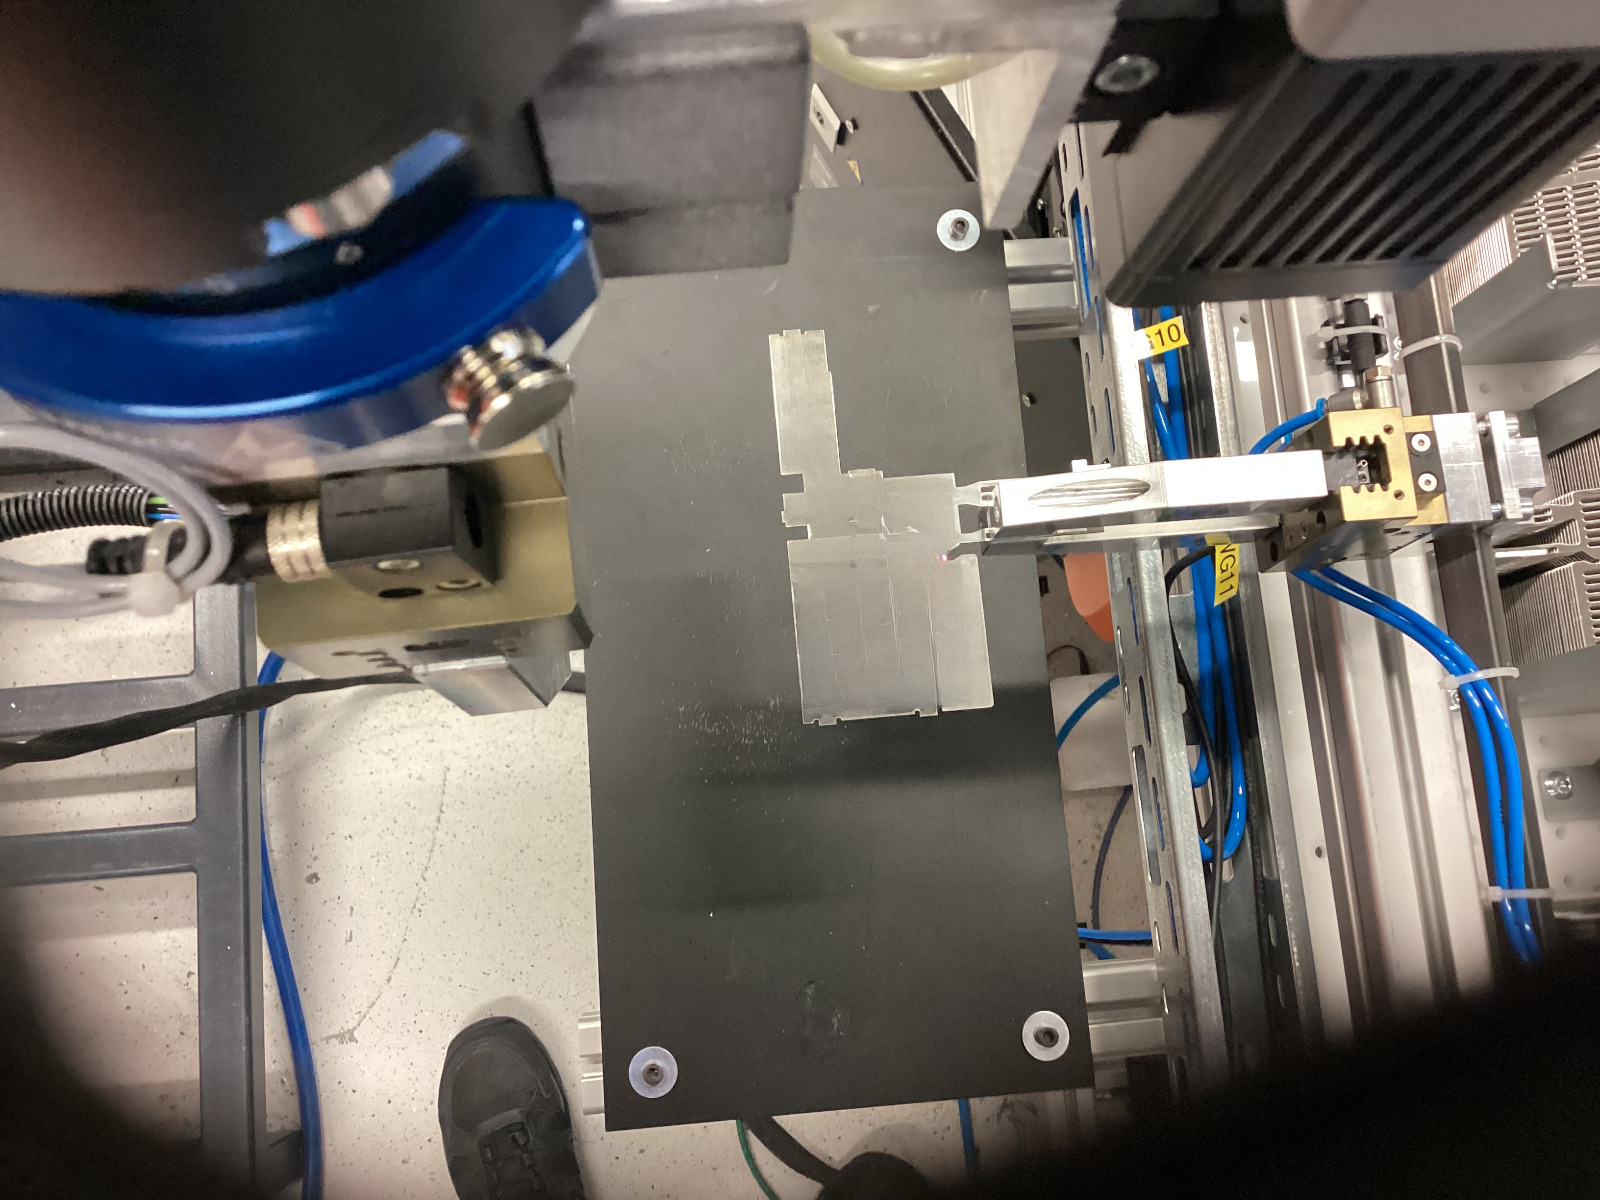
\includegraphics[width=\textwidth]{figures/sheet-pickup/scan.png}
        \caption{Scan sheet pattern using contour detector}
        \label{subfig:sheet-scan}
    \end{subfigure}\hspace{0.1cm}
    \begin{subfigure}[b]{0.48\textwidth}
        \centering
        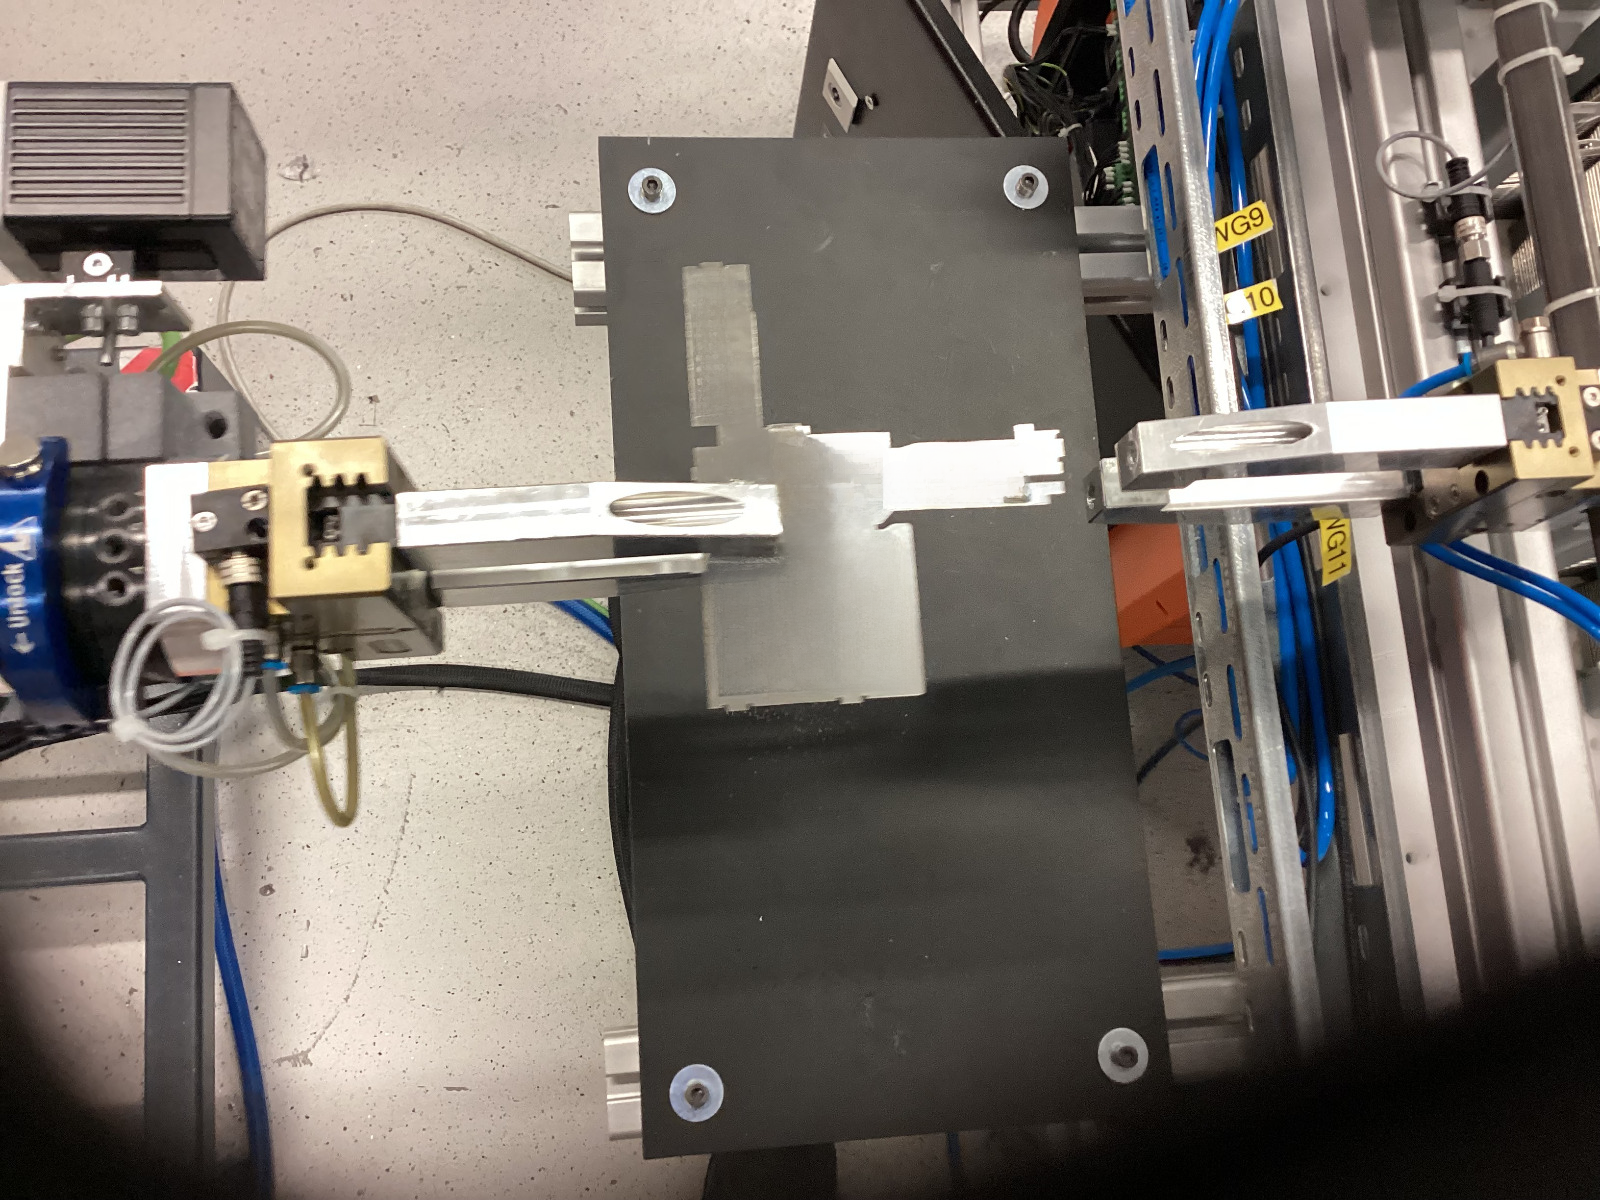
\includegraphics[width=\textwidth]{figures/sheet-pickup/taken.png}
        \caption{collect the sheet}
        \label{subfig:sheet-taken}
    \end{subfigure}
    \caption{Sheet pickup using robotic gripper}
    \label{fig:sheet-pickup}
\end{figure}

\begin{figure}[h]
    \centering
    \begin{subfigure}[b]{0.48\textwidth}
        \centering
        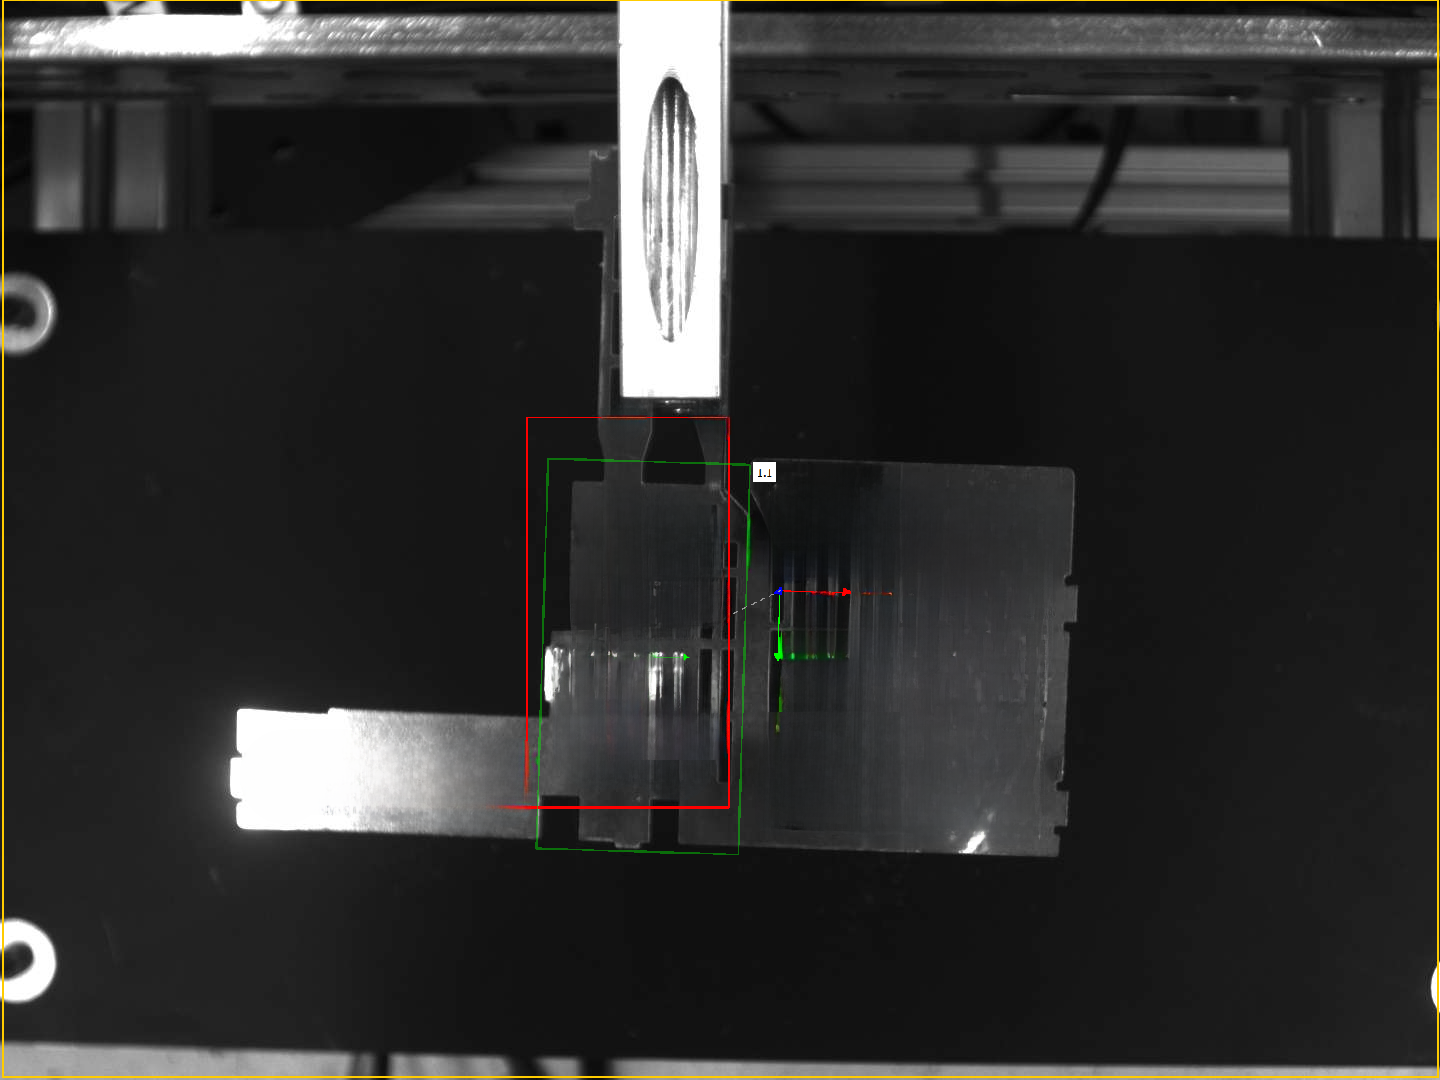
\includegraphics[width=\textwidth]{figures/sheet-pickup/camera-align.png}
        \caption{align camera}
        \label{subfig:sheet-1}
    \end{subfigure}\hspace{0.1cm}
    \begin{subfigure}[b]{0.48\textwidth}
        \centering
        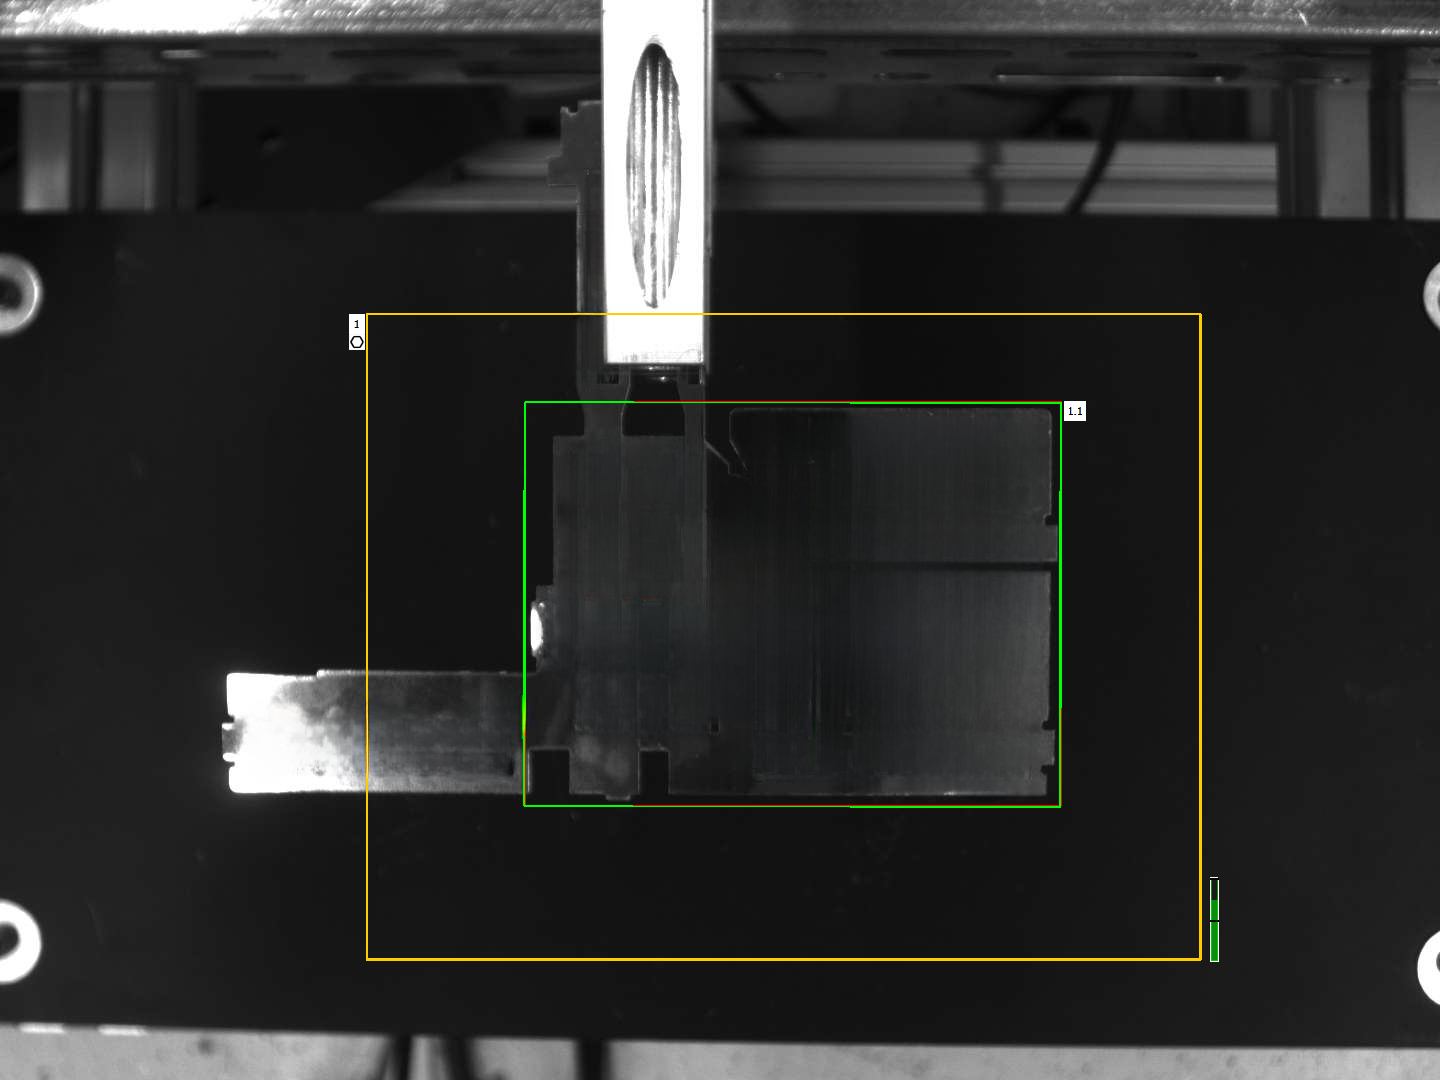
\includegraphics[width=\textwidth]{figures/sheet-pickup/sheet-pose.png}
        \caption{send sheet pose to pickup the sheet}
        \label{subfig:sheet-0}
    \end{subfigure}
    \caption{Sheet pattern detection using detector contour}
    \label{fig:sheet-scanning}
\end{figure}

The KR1410 uses the camera to detect and then securely pick the sheet. There are two stages of scanning as shown in figure \ref{fig:sheet-scanning}. A first scan aligns the camera perfectly with the sheet pattern. The second image capture detects the sheet with high accuracy in this way and sends the pose to the robot in world frame as shown in figure \ref{fig:sensoconfig-pattern}. Both stages uses detector contour to get the sheet pose.
The accuracy of the pickup is crucial for the success of the subsequent bending operations. Any misalignment at this stage could lead to errors in the final dimensions of the bent part.

\begin{figure}[h]
    \centering
    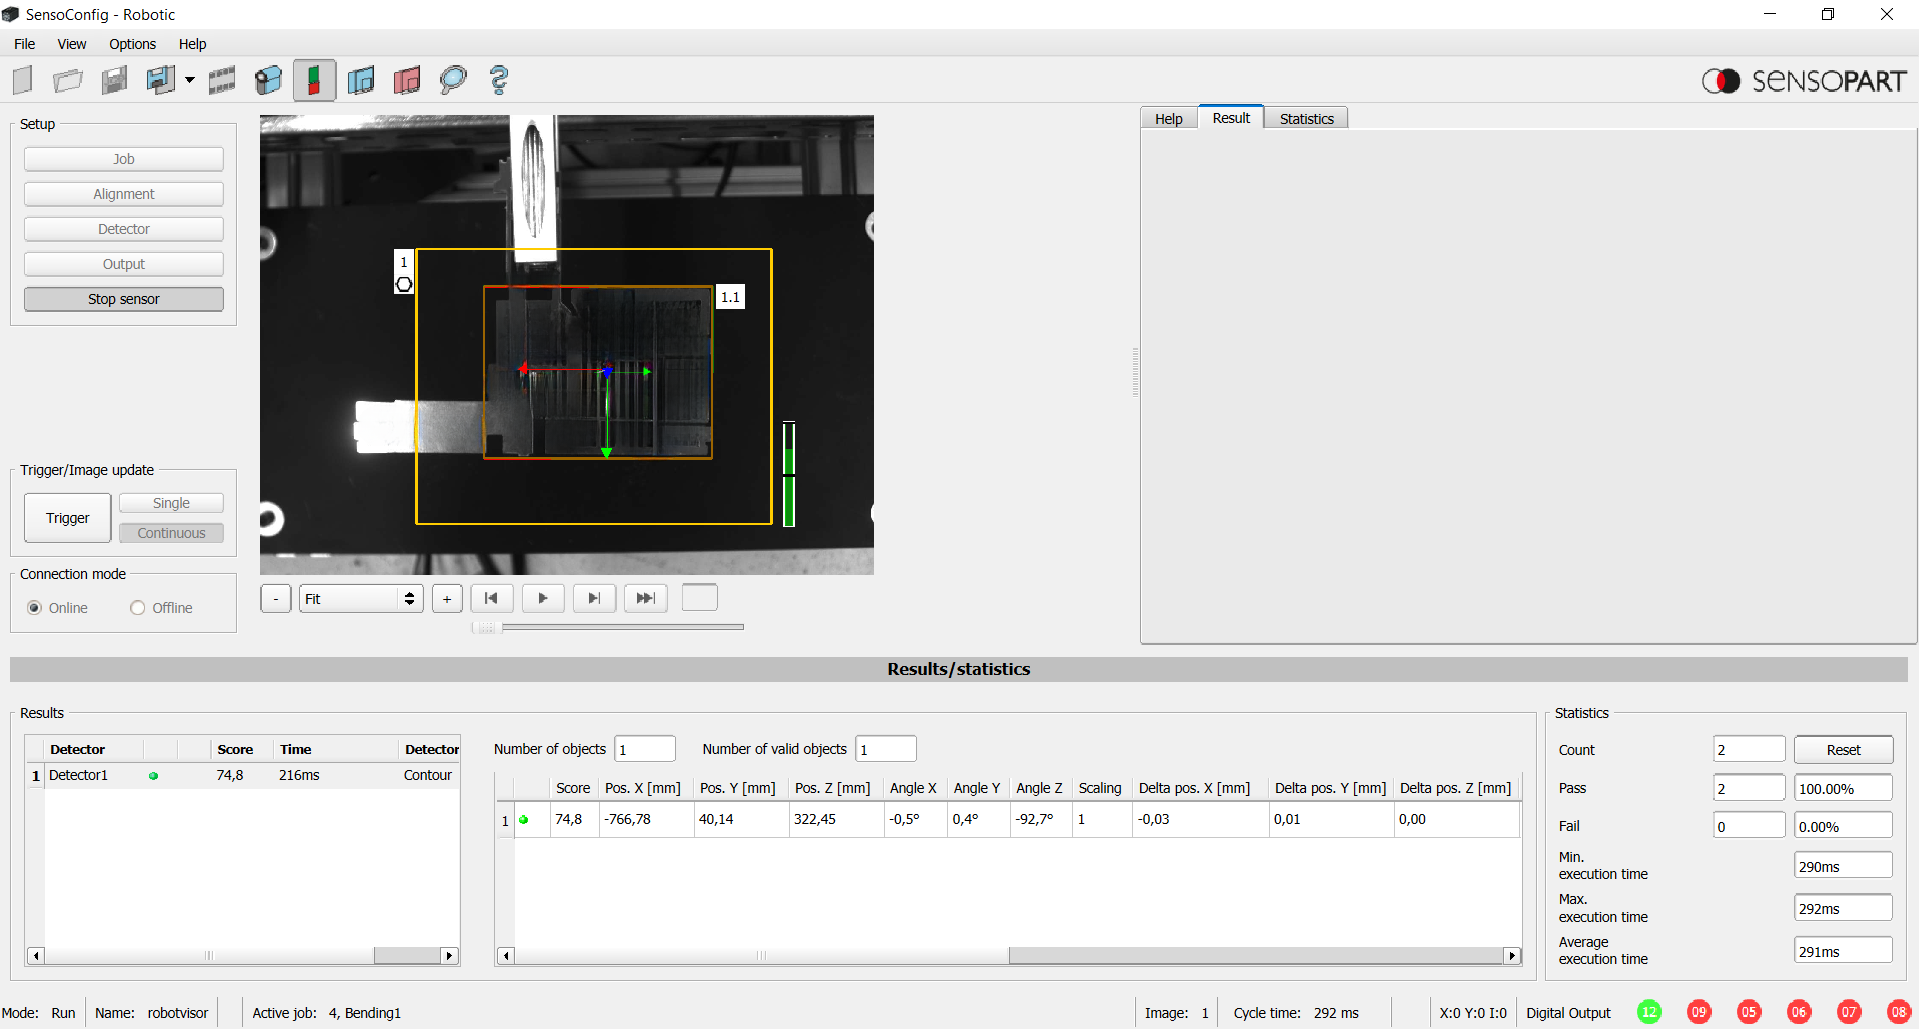
\includegraphics[width=\textwidth]{figures/sheet-pickup/sensoconfig.PNG}
    \caption{Detection and sending of sheet pose using telegram (SensoConfig)}
    \label{fig:sensoconfig-pattern}
\end{figure}

In some instances, to avoid collisions during next bending operation or for better handling of part, regripping of the sheet from a different position is required. This is where the unloading station gripper plays a crucial role in repositioning the sheet. The unloading station gripper is controlled from the KR1410 robot if the robot program state Int[0] is $\ge$3. (See table \ref{tab:kr1410-to-plc}). Otherwise the unloading station gripper is controlled by the PLC. 
\vspace{1\baselineskip}

First, the robot transfers the bent sheet to the unloading station gripper. Then, it is the same process as the sheet pickup in the first step of the bending cycle. The robot moves to the scanning pose, scans and aligns with the sheet, detects and grips the sheet and finally move out the part from the unloading station gripper.
Figure \ref{fig:sheet-pickup-before-placement} illustrates the step-by-step process of regrasping of sheet metal part for sheet placement in the storage station after all the bending operations are complete.


\begin{figure}[h]
    \centering
    \begin{subfigure}[b]{0.32\textwidth}
        \centering
        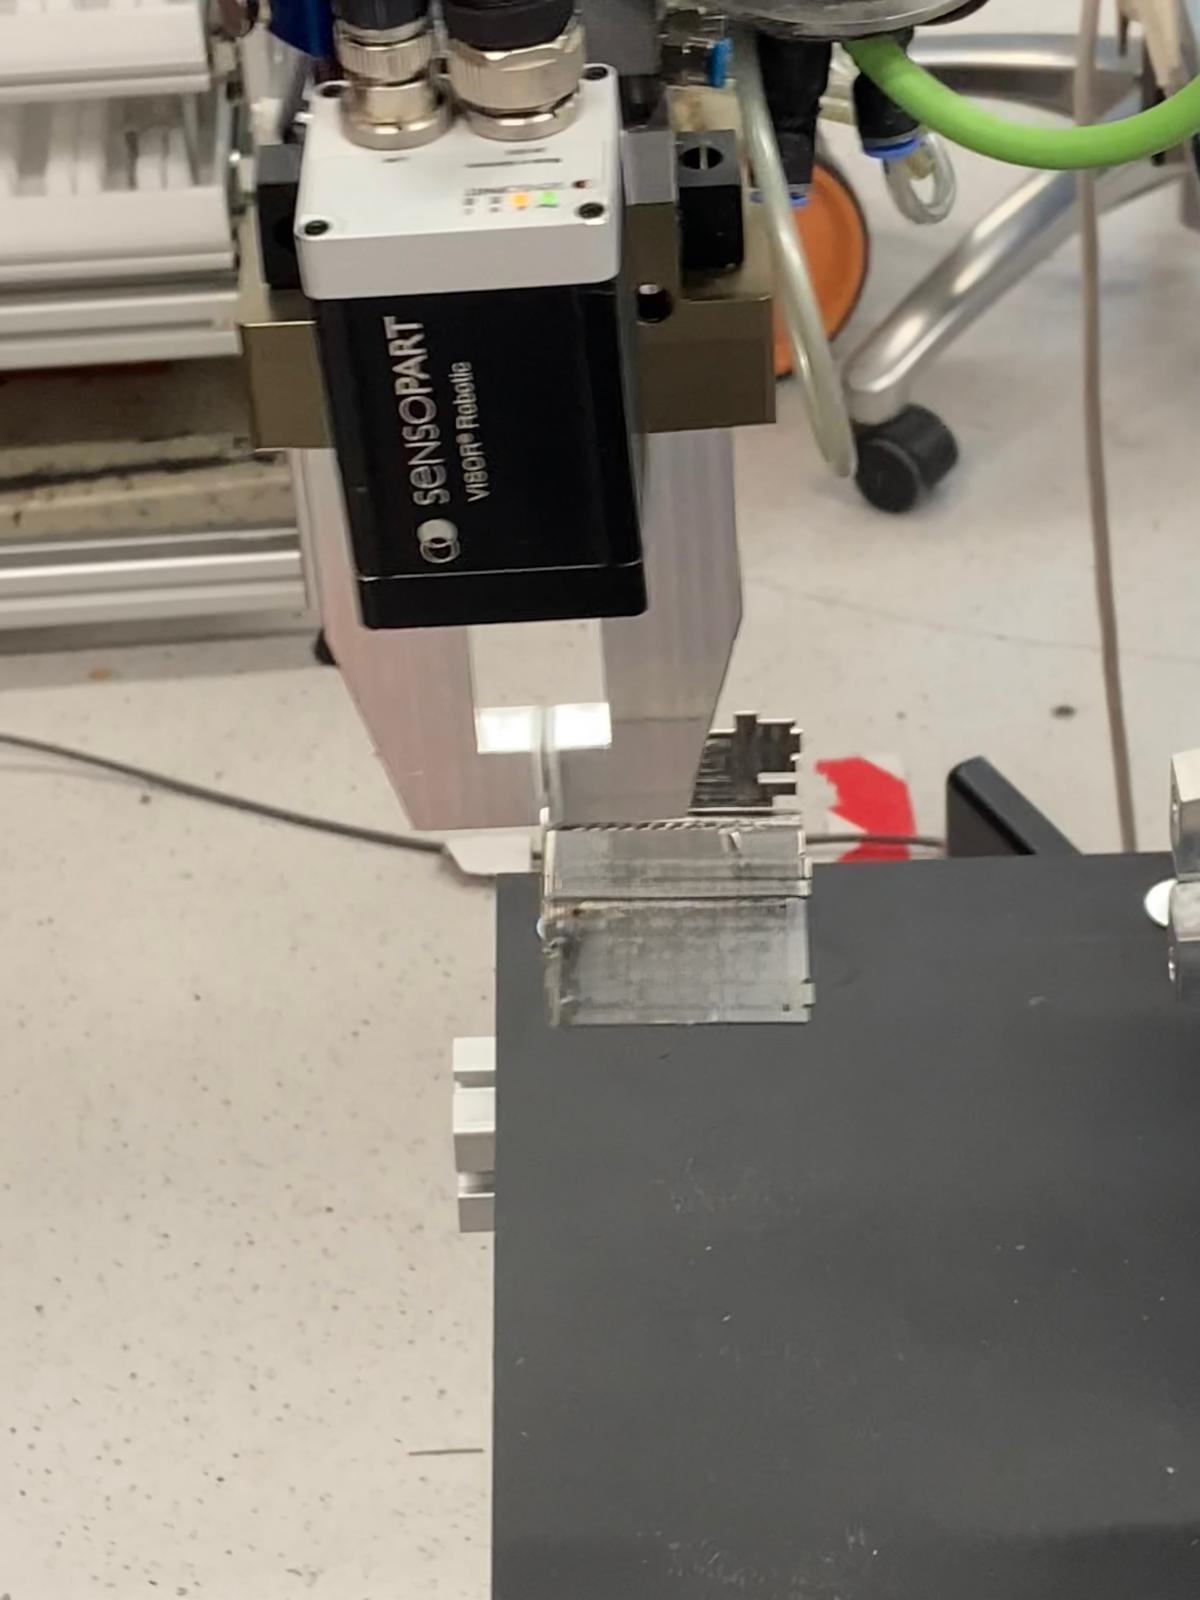
\includegraphics[width=\textwidth]{figures/sheet-pickup/sheet-placement01.png}
        \caption{Go to unloading station gripper}
        \label{subfig:sheet-placement01}
    \end{subfigure}\hspace{0.1cm}
    \begin{subfigure}[b]{0.32\textwidth}
        \centering
        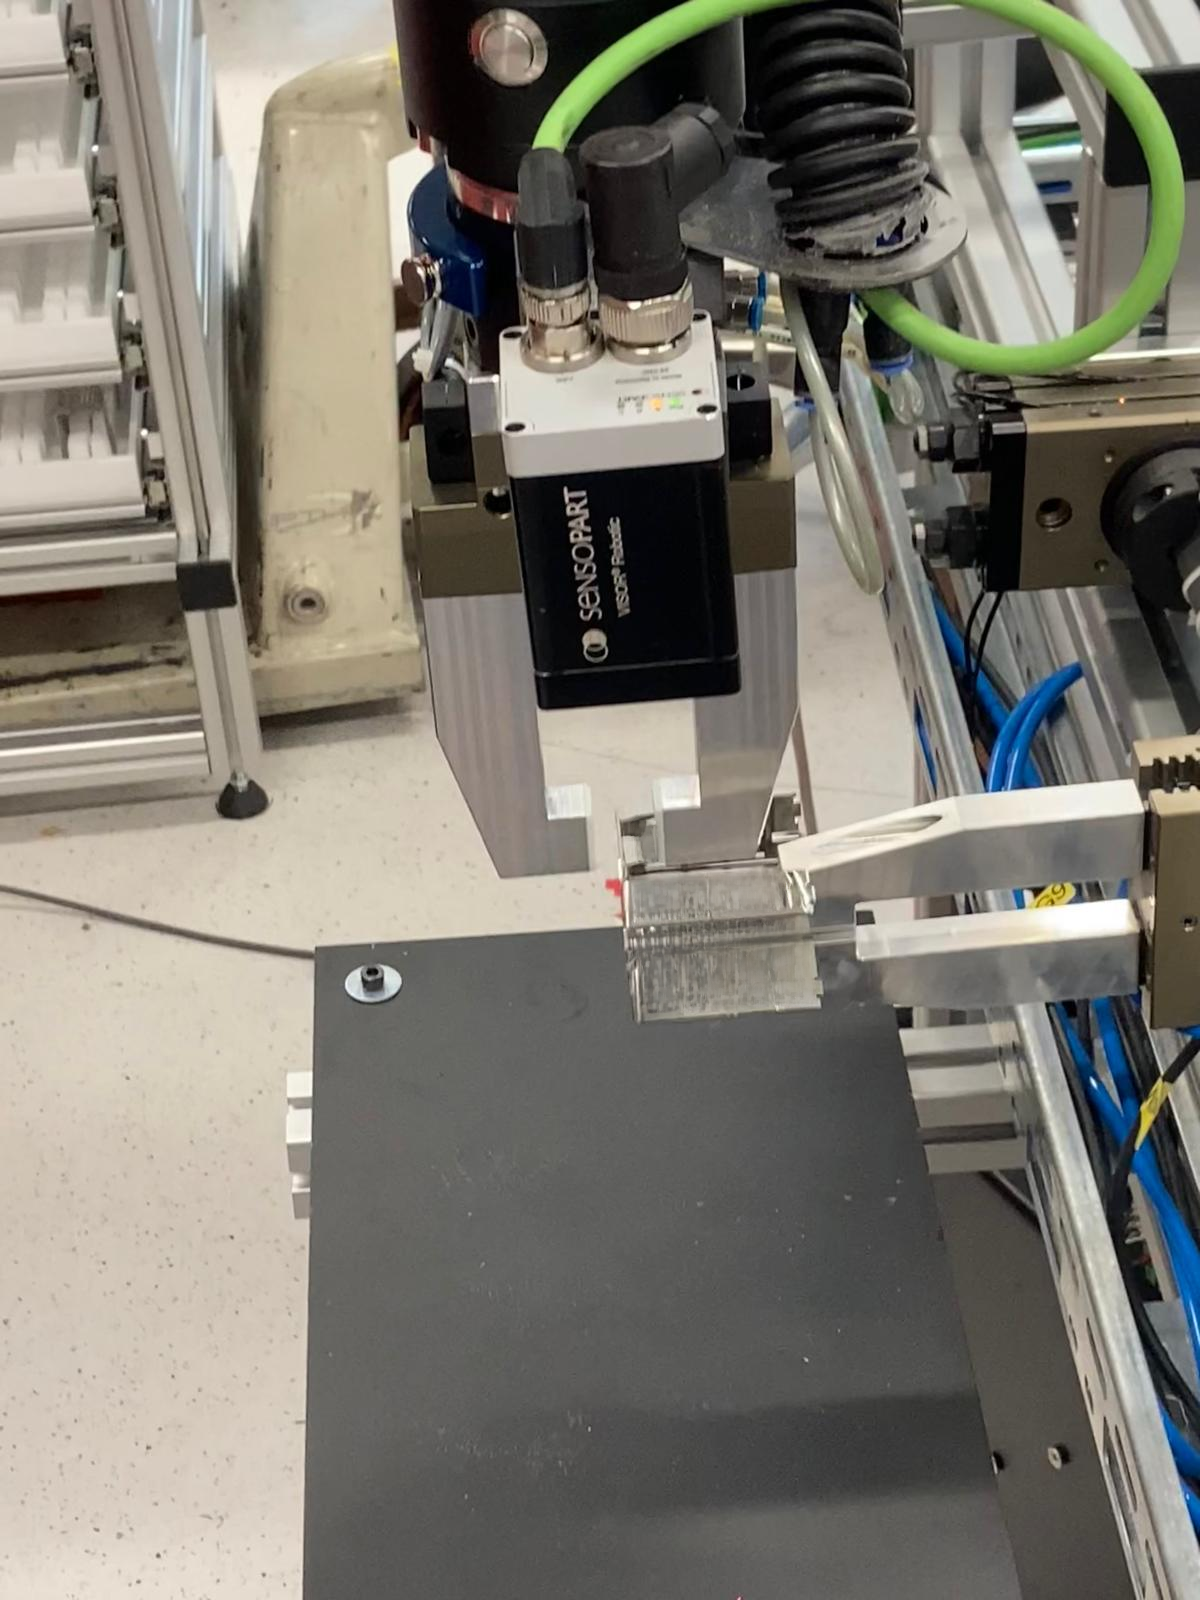
\includegraphics[width=\textwidth]{figures/sheet-pickup/sheet-placement02.png}
        \caption{transfer sheet to unloading station gripper}
        \label{subfig:sheet-placement02}
    \end{subfigure}\hspace{0.1cm}
    \vspace{1cm}
    \begin{subfigure}[b]{0.32\textwidth}
        \centering
        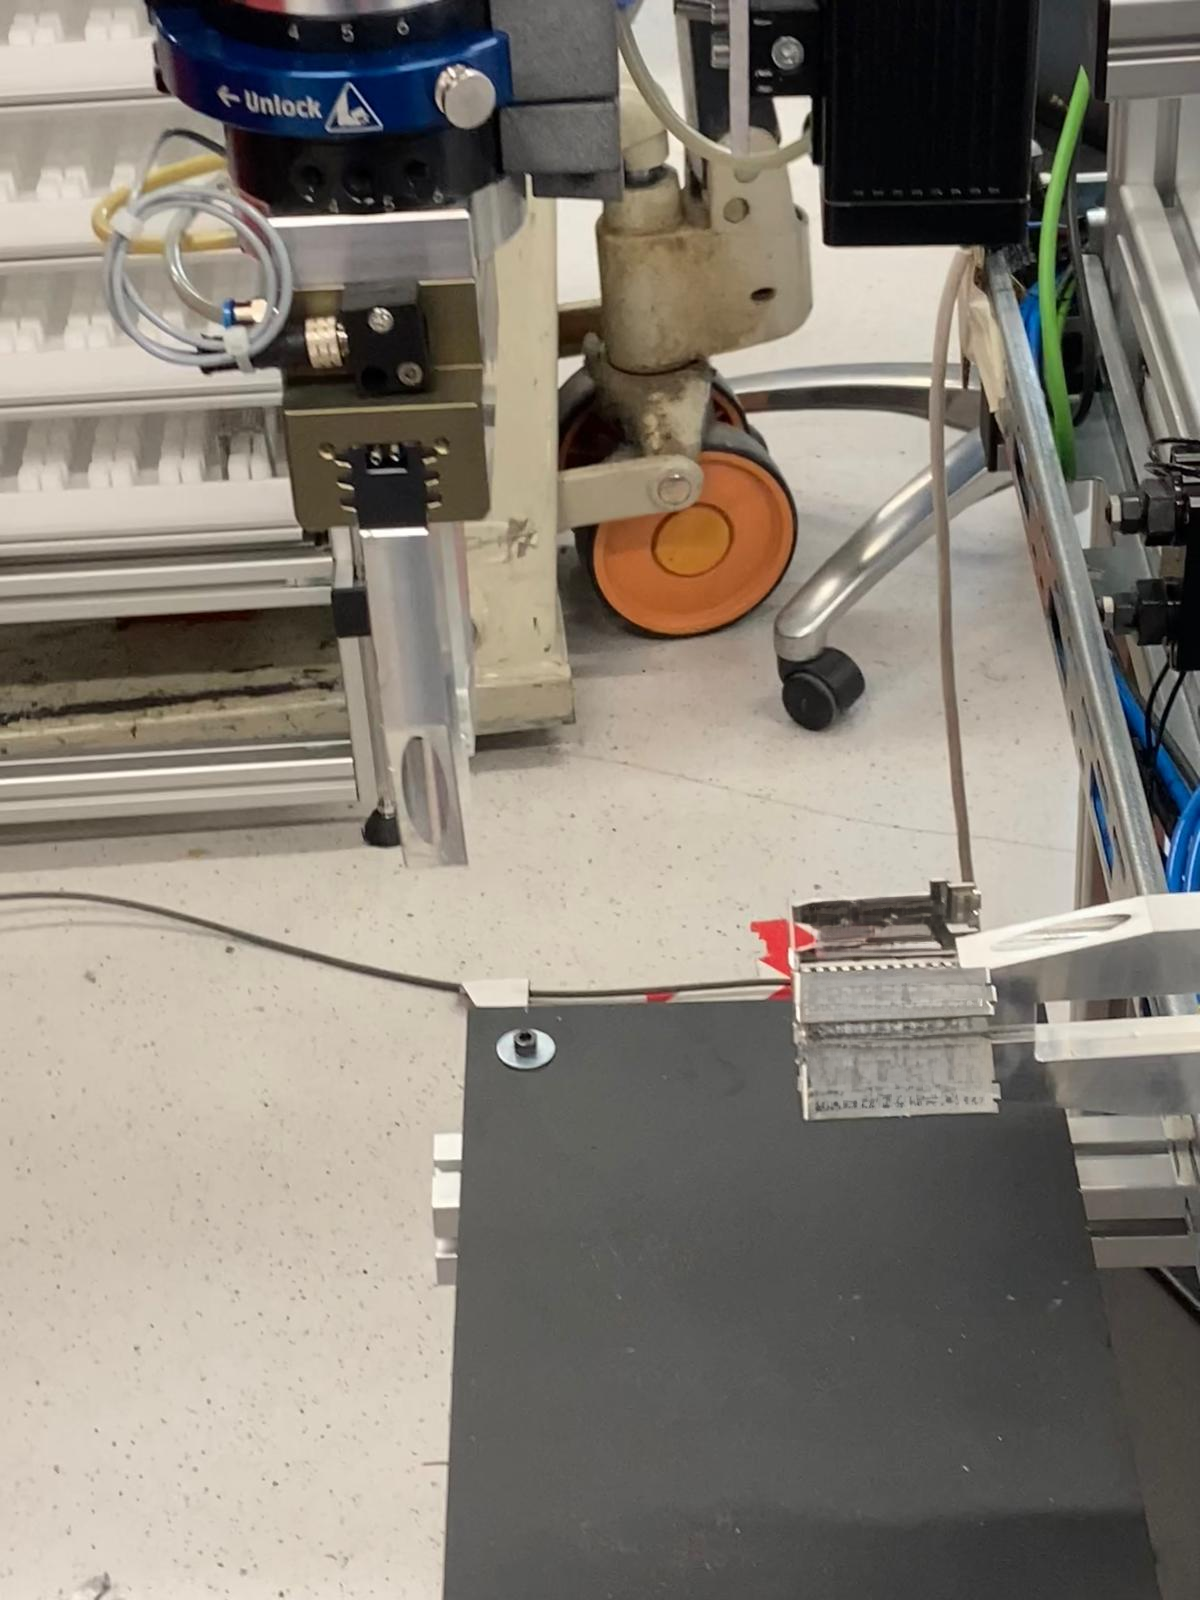
\includegraphics[width=\textwidth]{figures/sheet-pickup/sheet-placement03.png}
        \caption{Scan sheet pattern and align camera}
        % \vspace{-0.45cm}
        \label{subfig:sheet-placement03}
    \end{subfigure}\hspace{0.1cm}
    \begin{subfigure}[b]{0.32\textwidth}
        \centering
        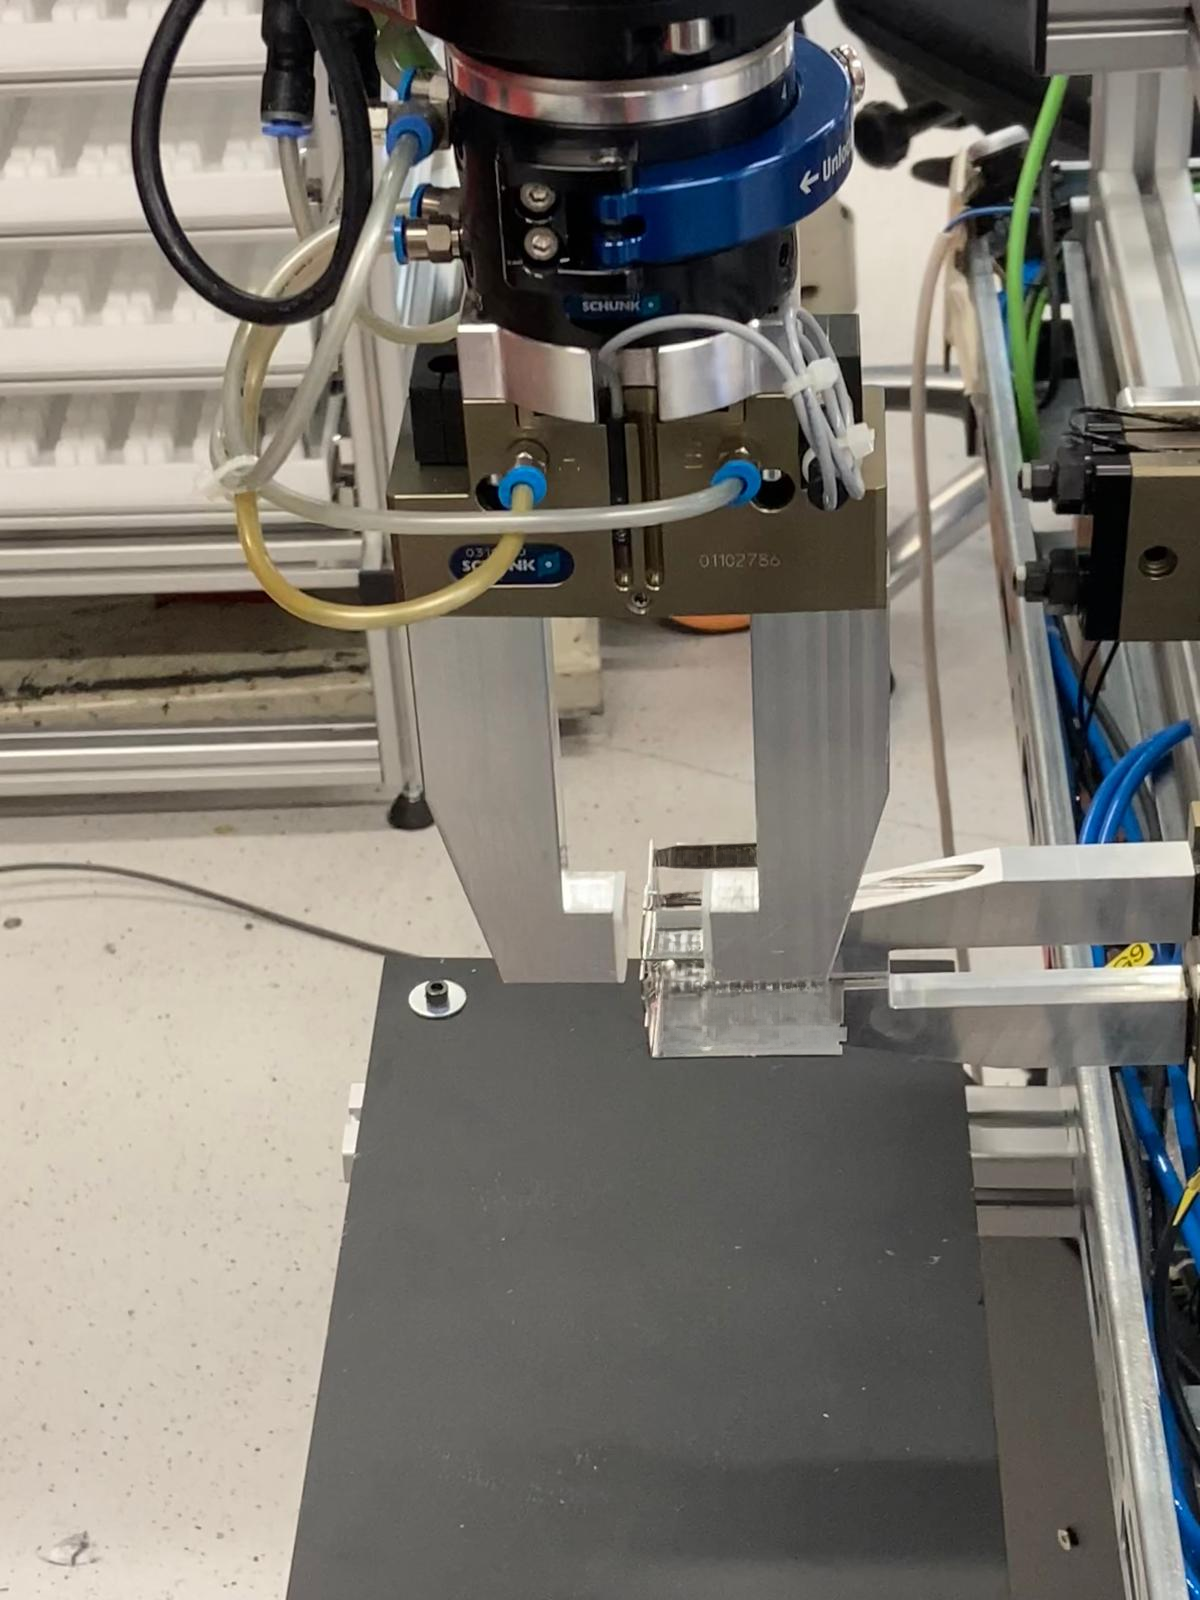
\includegraphics[width=\textwidth]{figures/sheet-pickup/sheet-placement04.png}
        \caption{Scan again for sheet detection}
        \label{subfig:sheet-placement04}
    \end{subfigure}\hspace{0.1cm}
    \vspace{0.75cm}
    \begin{subfigure}[b]{0.32\textwidth}
        \centering
        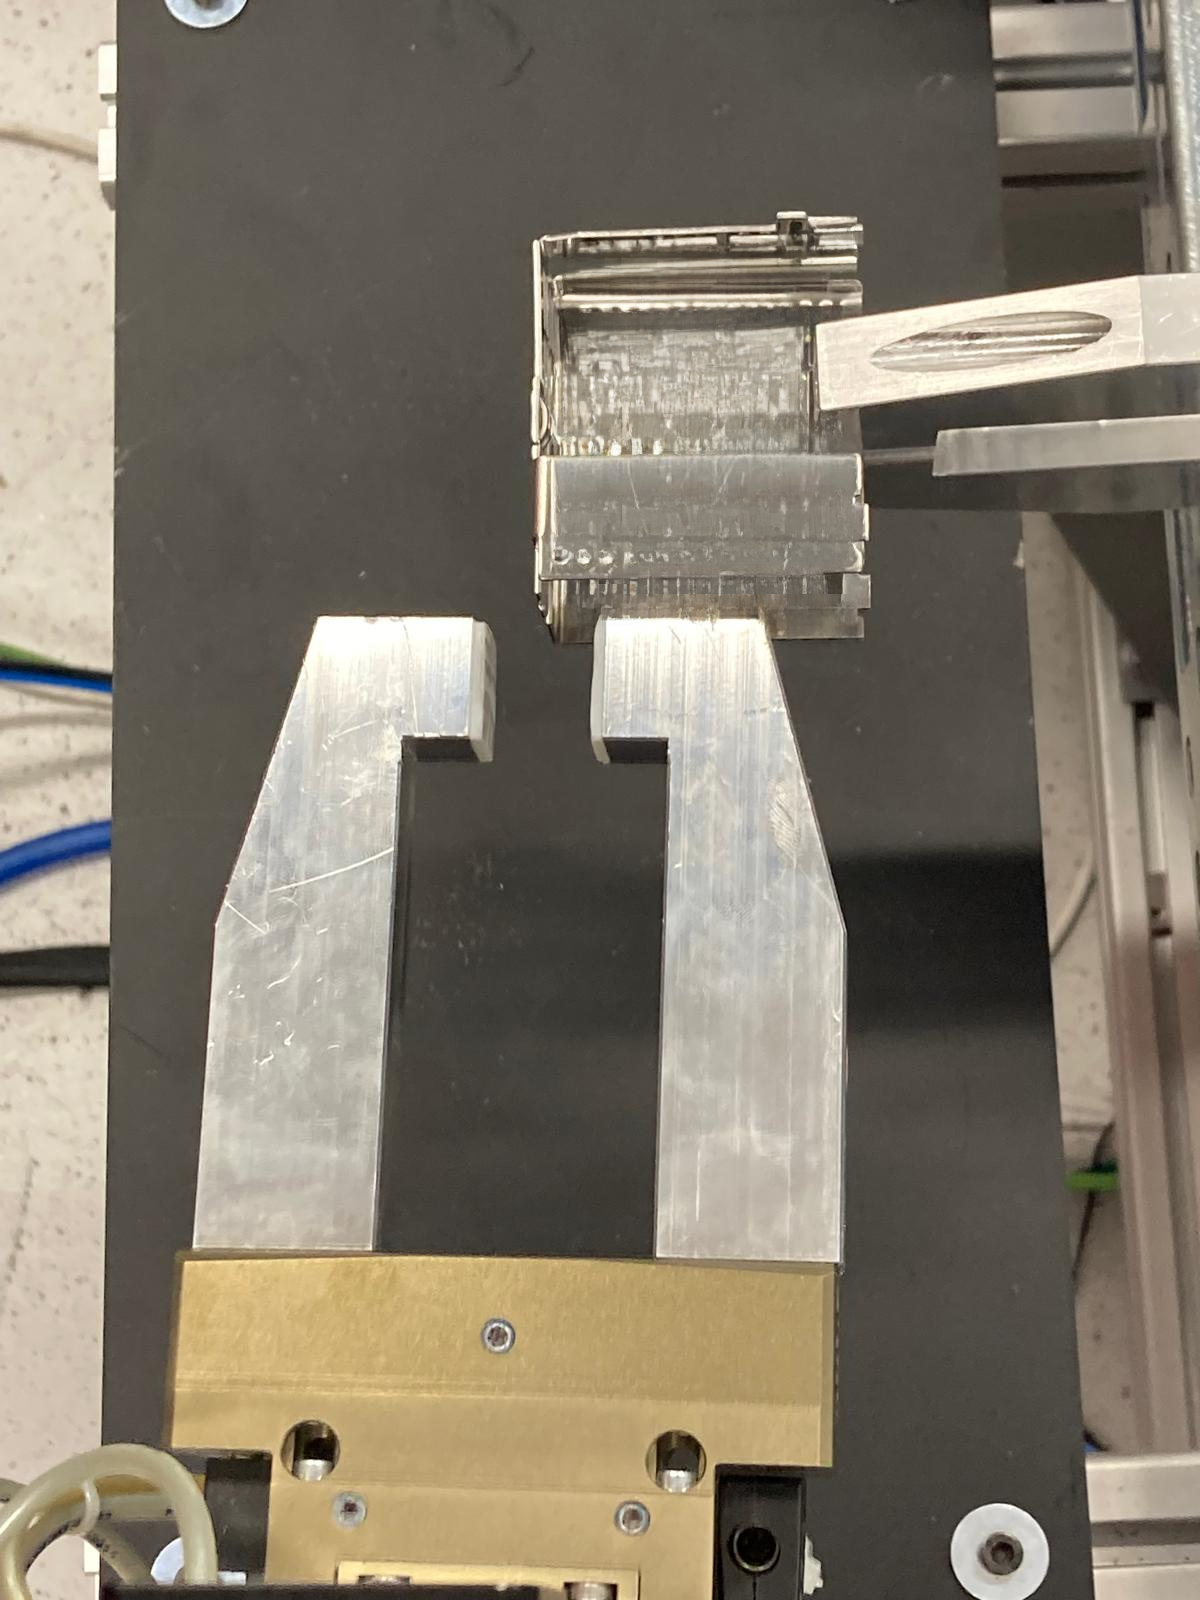
\includegraphics[width=\textwidth]{figures/sheet-pickup/sheet-placement05.png}
        \caption{Grasp sheet from unloading station gripper}
        \label{subfig:sheet-placement05}
    \end{subfigure}\hspace{0.1cm}
    \begin{subfigure}[b]{0.32\textwidth}
        \centering
        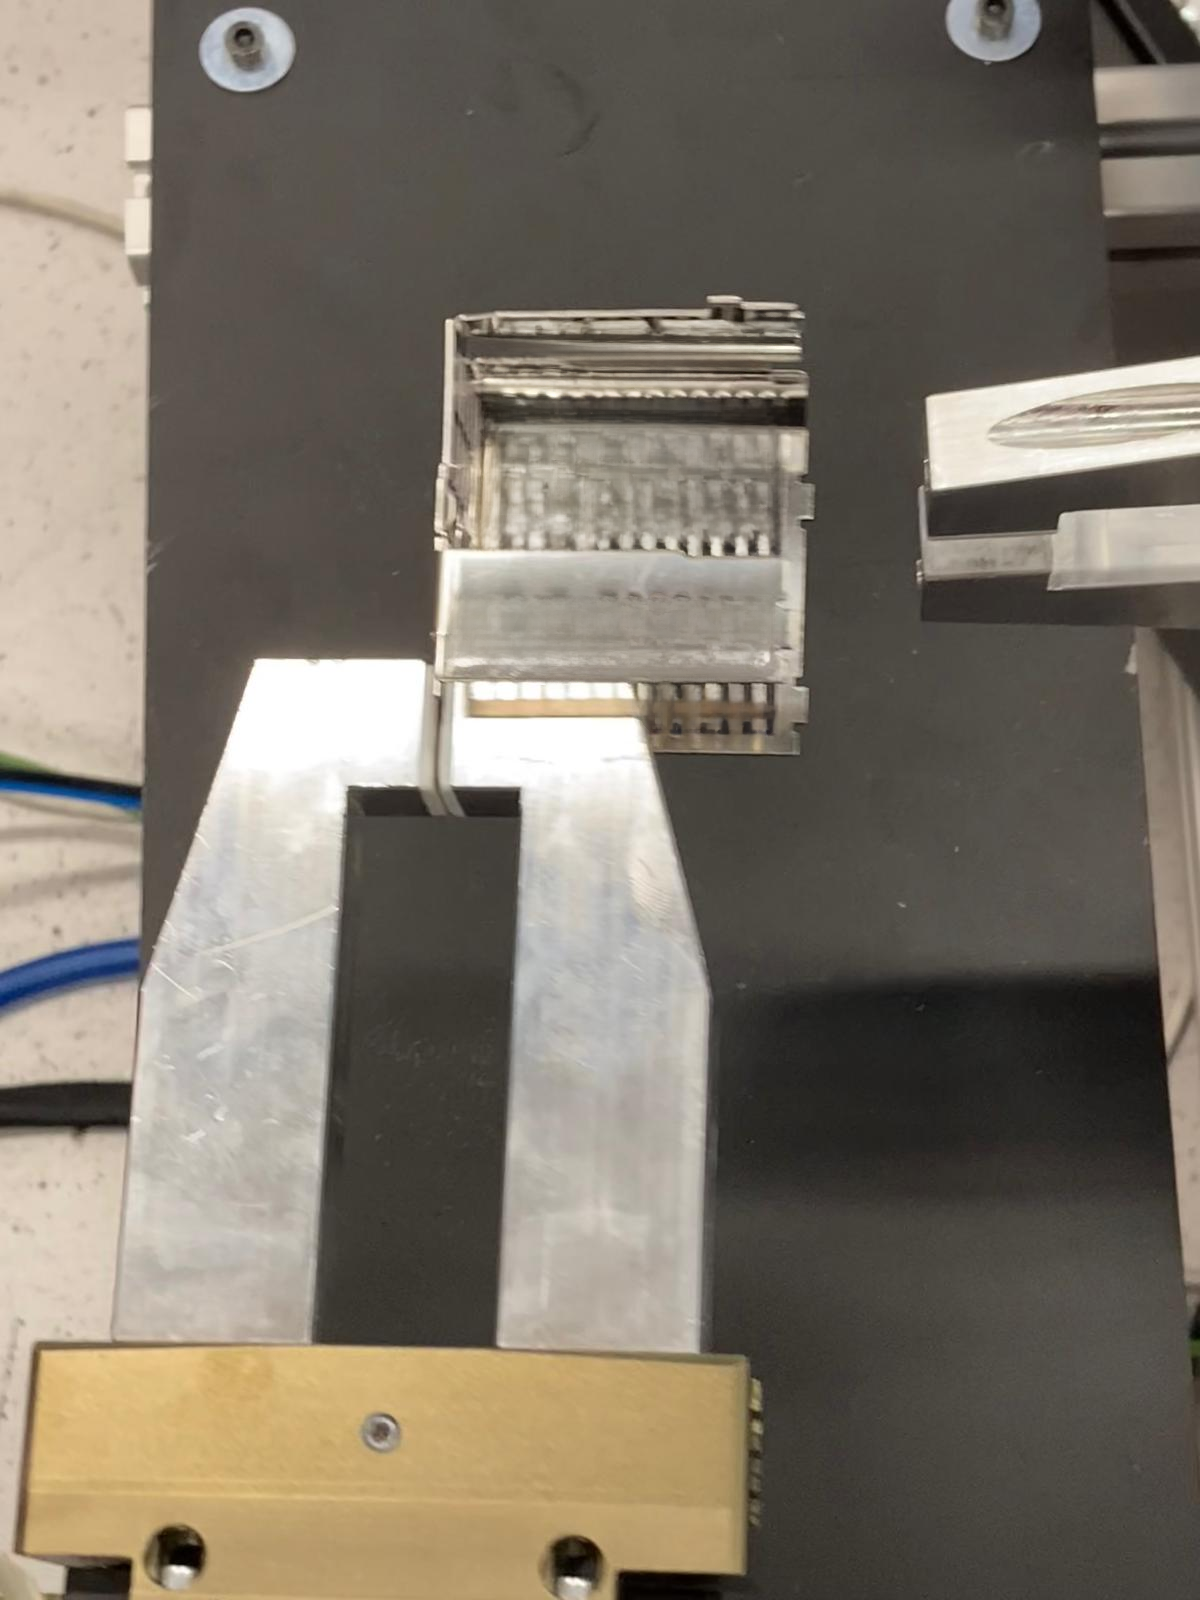
\includegraphics[width=\textwidth]{figures/sheet-pickup/sheet-placement06.png}
        \caption{Move out}
        \label{subfig:sheet-placement06}
        \vspace{0.45cm}
    \end{subfigure}\hspace{0.1cm}
    \caption{Regrasping bent sheet from a different position before placement in drawer}
    \label{fig:sheet-pickup-before-placement}
\end{figure}

\FloatBarrier  % Force all figures of the first section to be placed before the next section

\subsection{Bending Operation}
\label{subsec:bending-operation}
% Bending operations

The test part undergoes a sequence of six bendings, with different angles and setups. Specifically, bending operations 1, 5, and 6 are performed at bending station 1 and undergoes a bending of 90° angle, whereas bending operations 2 and 3 are performed at bending station 2 with a bending of 135°, and the fourth bending operation is simply done to flatten the sheet metal part.

The first step before the bending for all bending operations is the correct alignment of the part in the backgauges of the bending machine. The bending machine program is automatically set by the terminal operating robot. Once the correct sequence is selected in the terminal of the bending machine, PLC send a signal to the KR1410 robot which gives permission to align the sheet in the backgauges.
Then only the KR1410 arm secures the part in the backgauges of the bending machine.

\begin{figure}[h]
    \centering
    \begin{subfigure}[b]{0.32\textwidth}
        \centering
        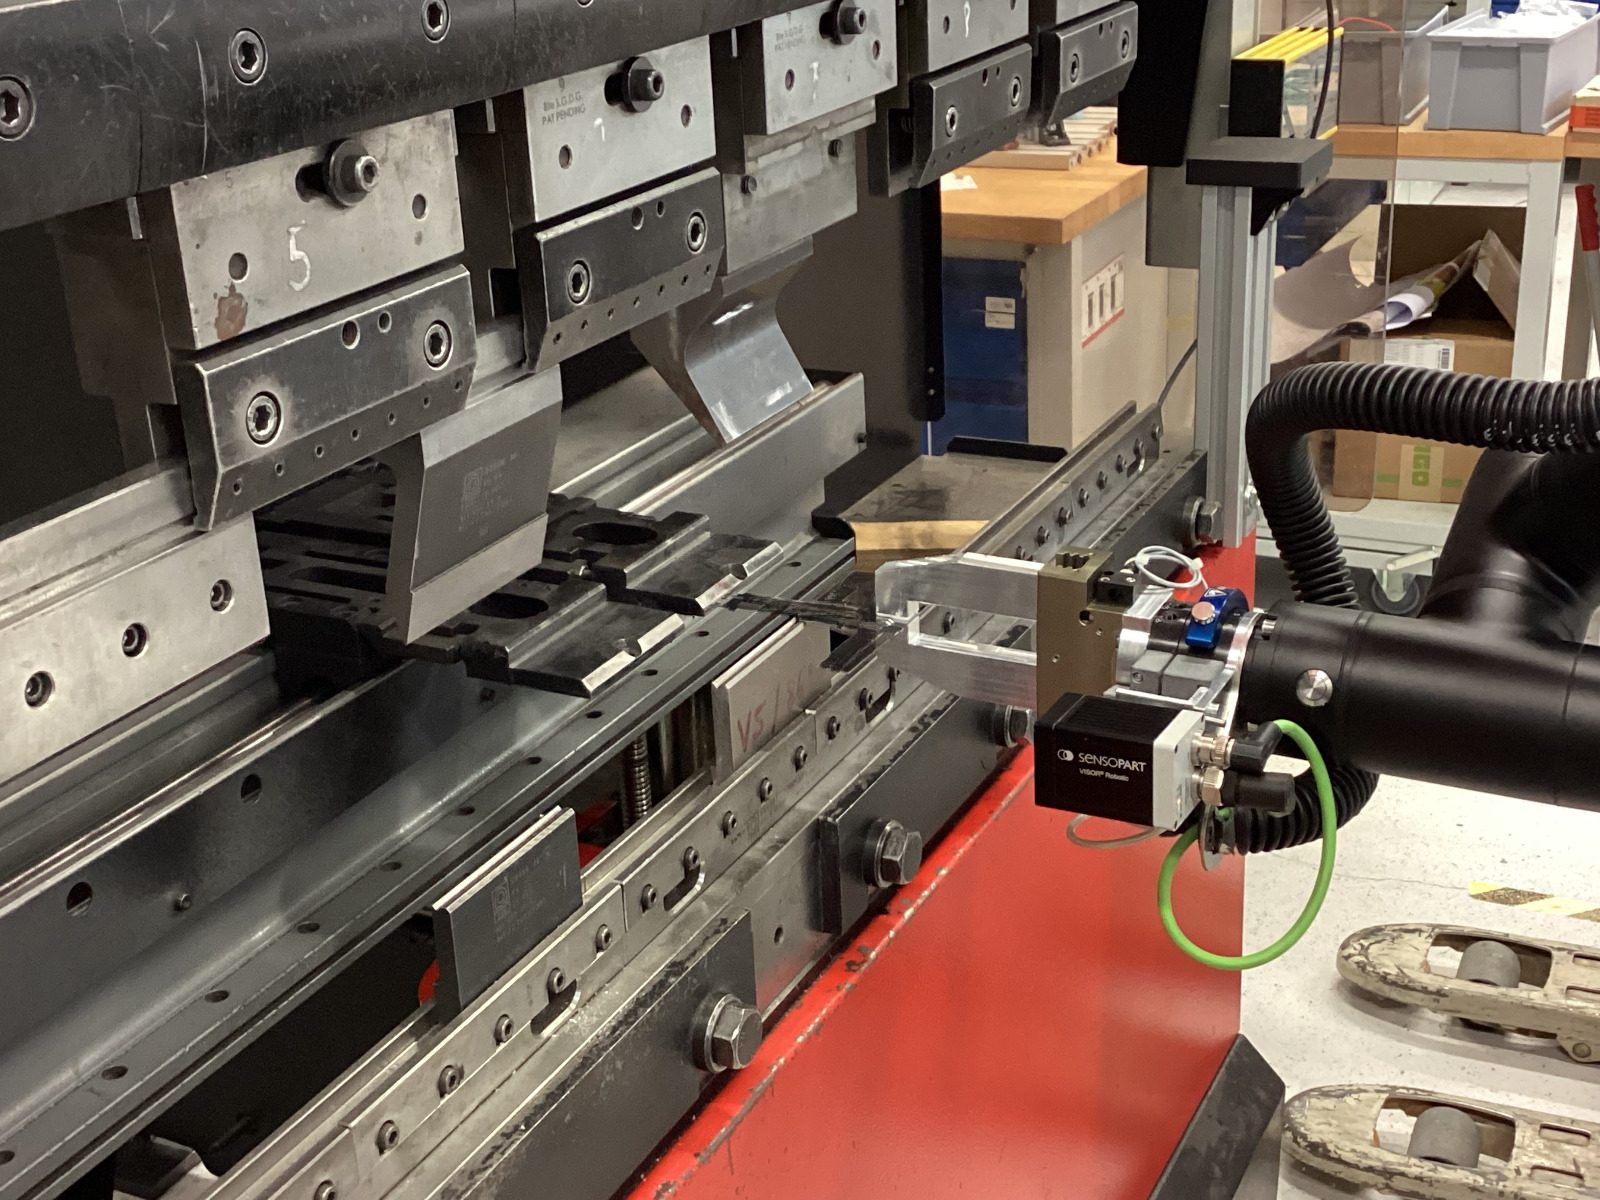
\includegraphics[width=\textwidth]{figures/bending/bending1-002.png}
        \caption{Go to bending station 1}
        \label{subfig:bending1-before}
    \end{subfigure}\hspace{0.1cm}
    \begin{subfigure}[b]{0.32\textwidth}
        \centering
        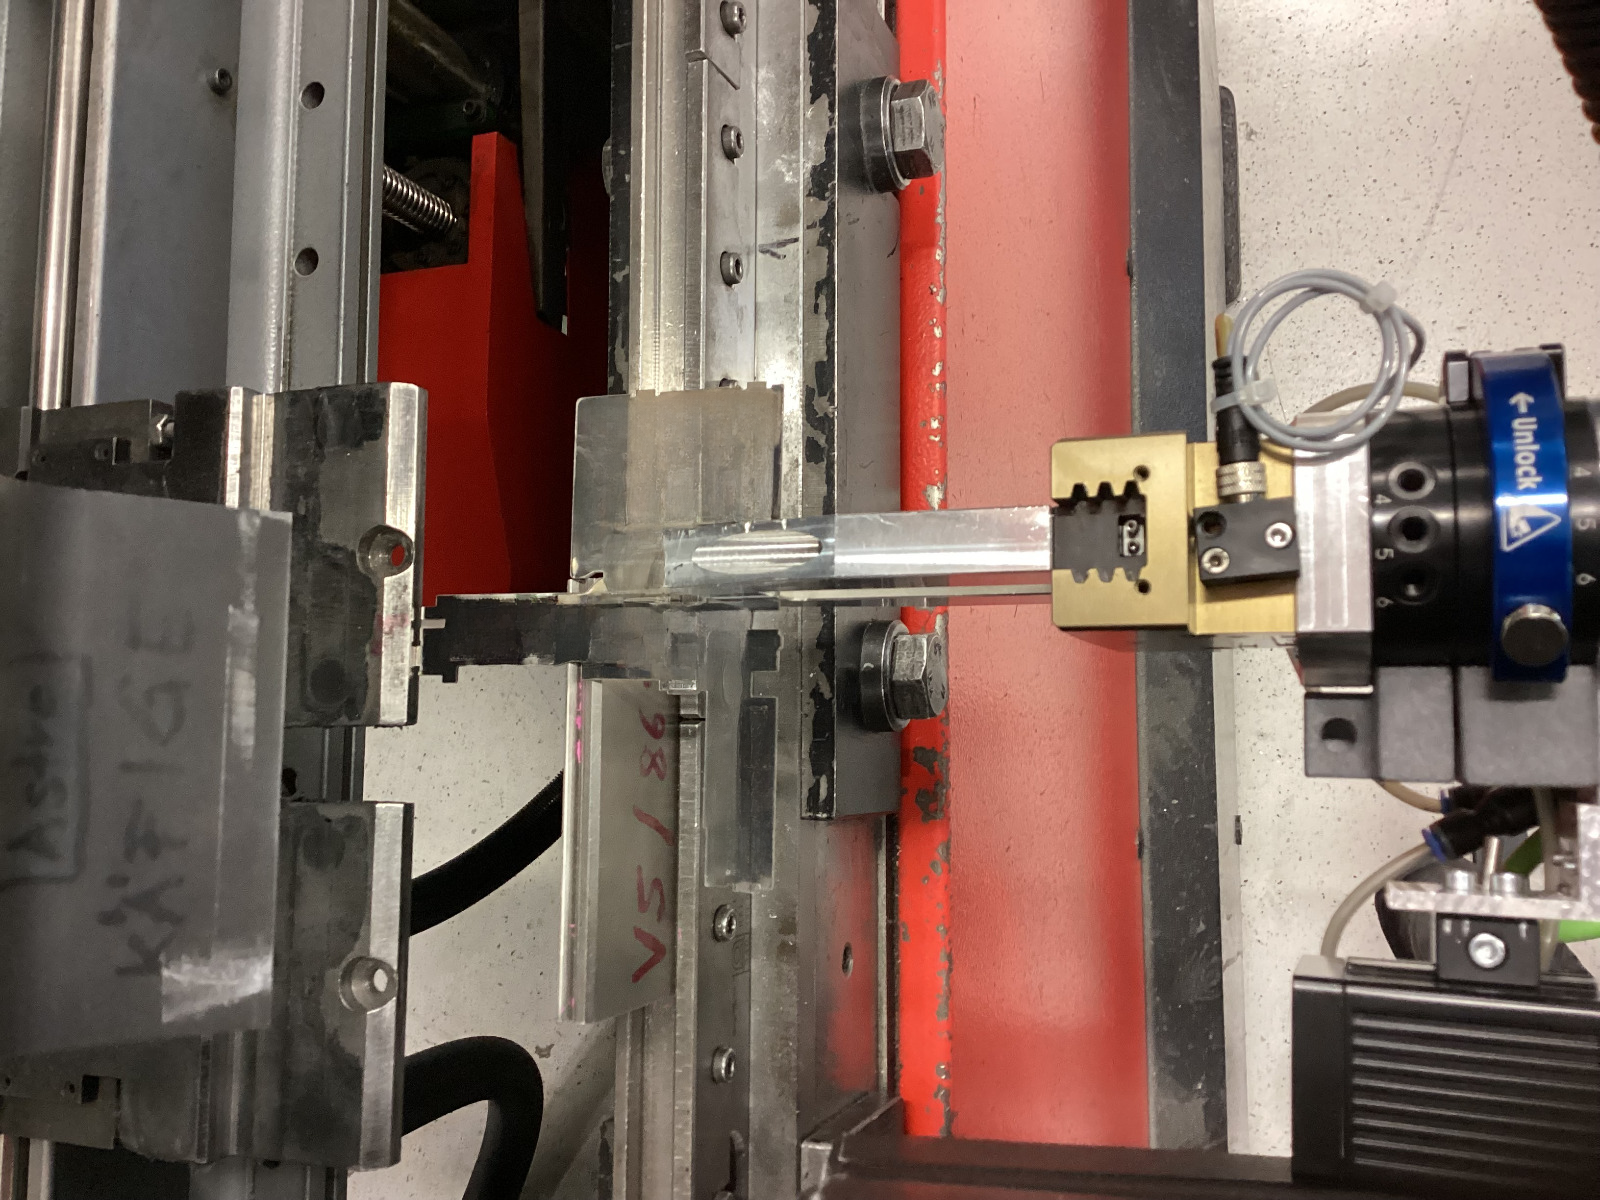
\includegraphics[width=\textwidth]{figures/bending/bending1-003.png}
        \caption{bend the sheet metal part}
        \label{subfig:bending1}
    \end{subfigure}\hspace{0.1cm}
    \begin{subfigure}[b]{0.32\textwidth}
        \centering
        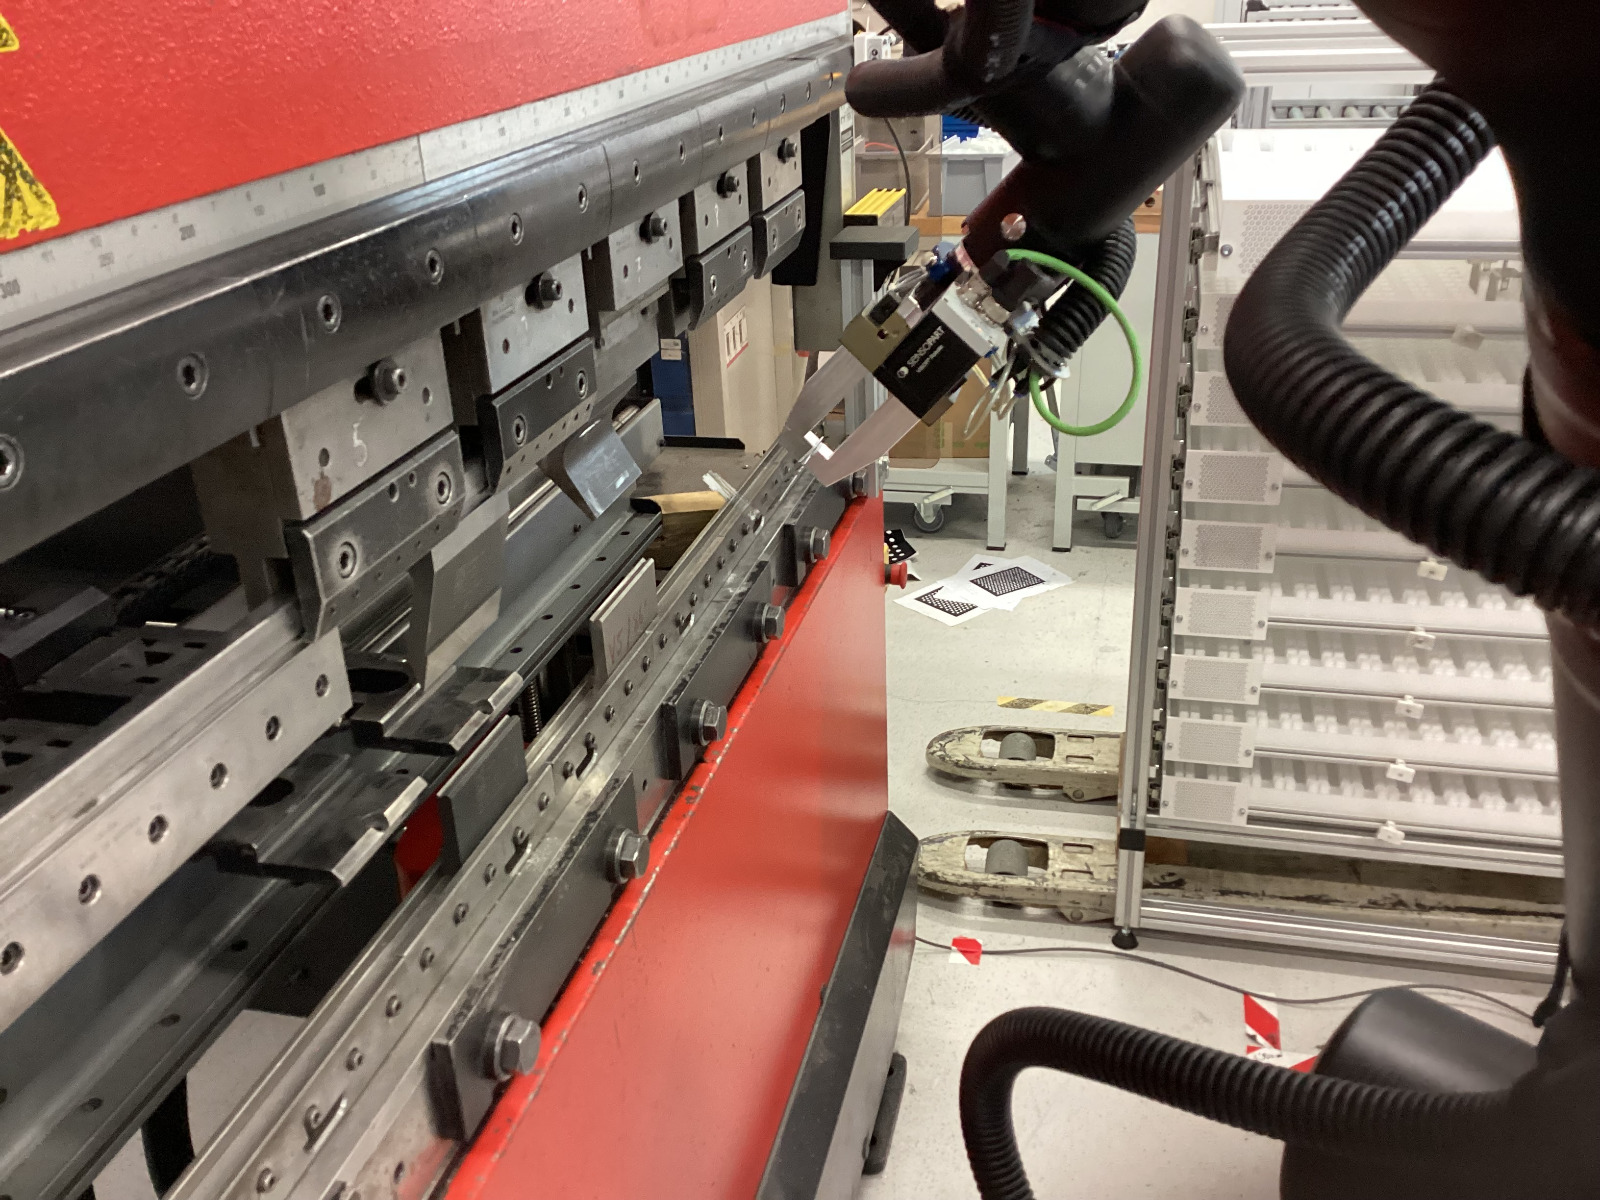
\includegraphics[width=\textwidth]{figures/bending/bending1-001.png}
        \caption{take away the bent sheet}
        \label{subfig:bending1-after}
    \end{subfigure}\hspace{0.1cm}
    \caption{Bending operation number 1 at bending station 1}
    \label{fig:bending-operation-1}
\end{figure}

\begin{figure}[h]
    \centering
    \begin{subfigure}[b]{0.32\textwidth}
        \centering
        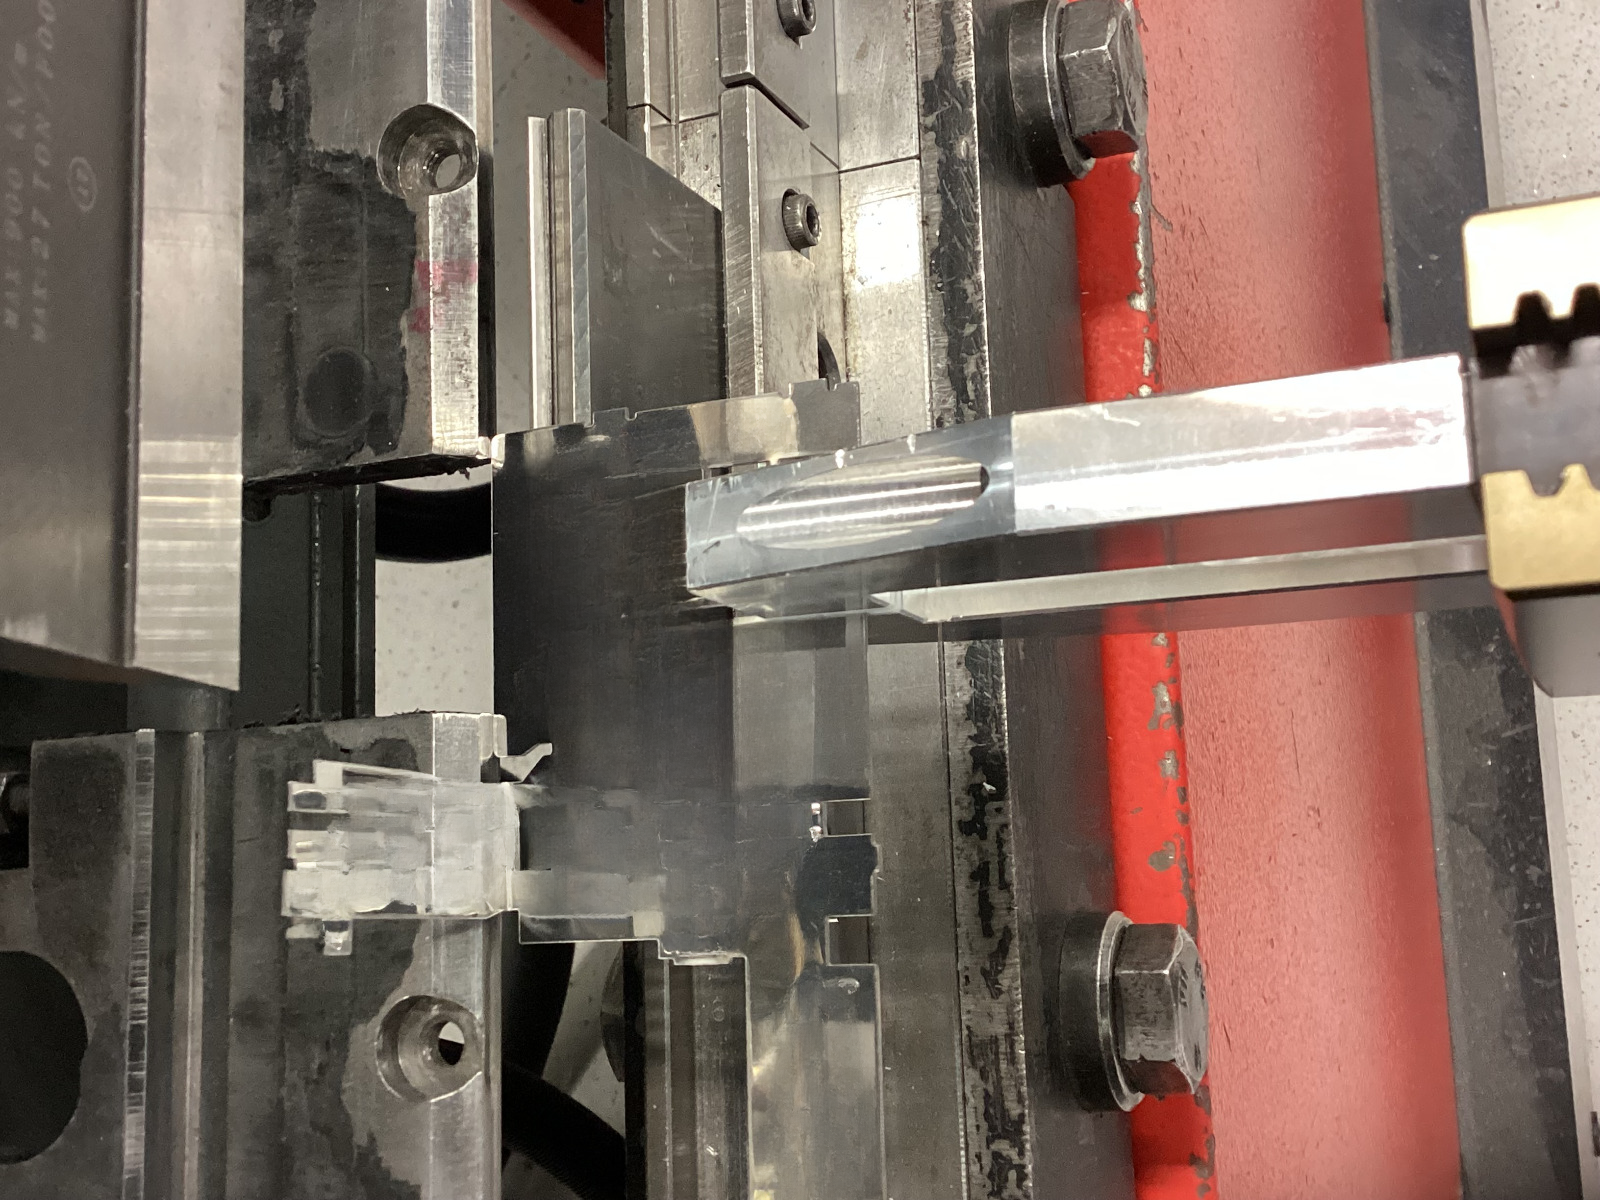
\includegraphics[width=\textwidth]{figures/bending/bending2-003.png}
        \caption{Go to bending station 2}
        \label{subfig:bending2-before}
    \end{subfigure}\hspace{0.1cm}
    \begin{subfigure}[b]{0.32\textwidth}
        \centering
        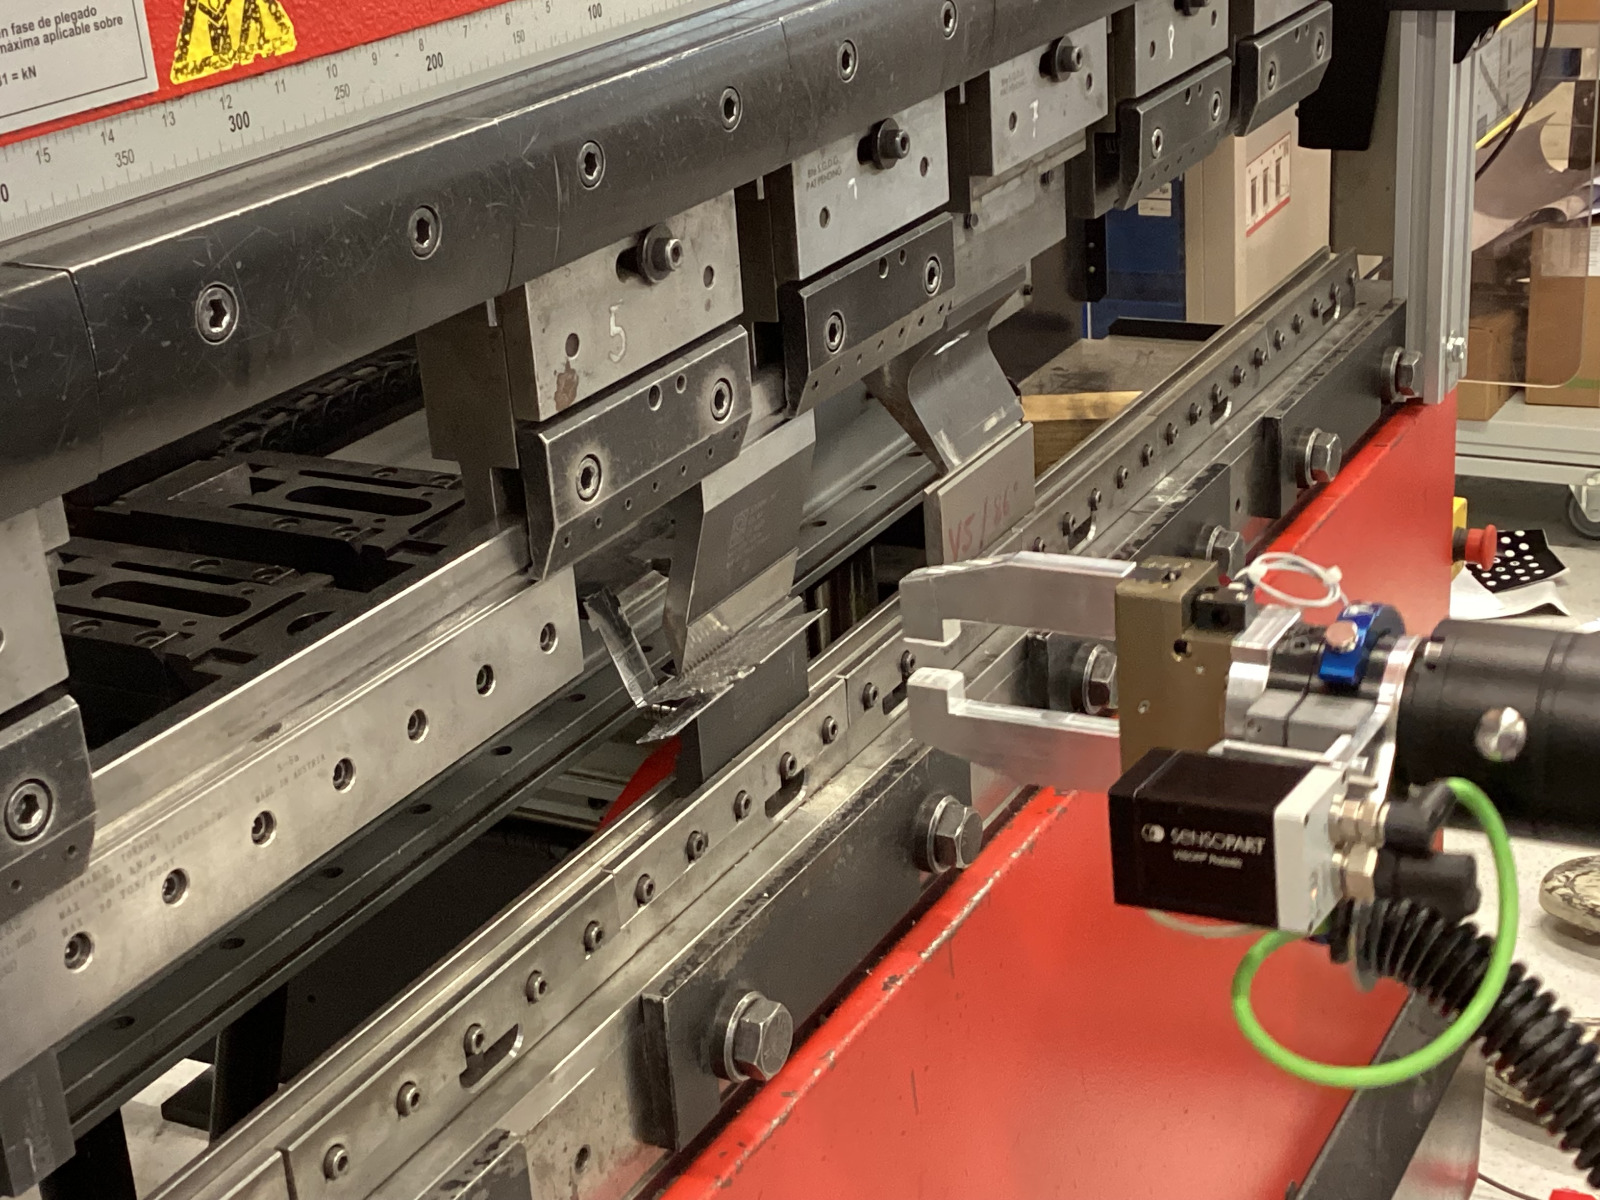
\includegraphics[width=\textwidth]{figures/bending/bending2-001.png}
        \caption{bend the sheet metal part}
        \label{subfig:bending2}
    \end{subfigure}\hspace{0.1cm}
    \begin{subfigure}[b]{0.32\textwidth}
        \centering
        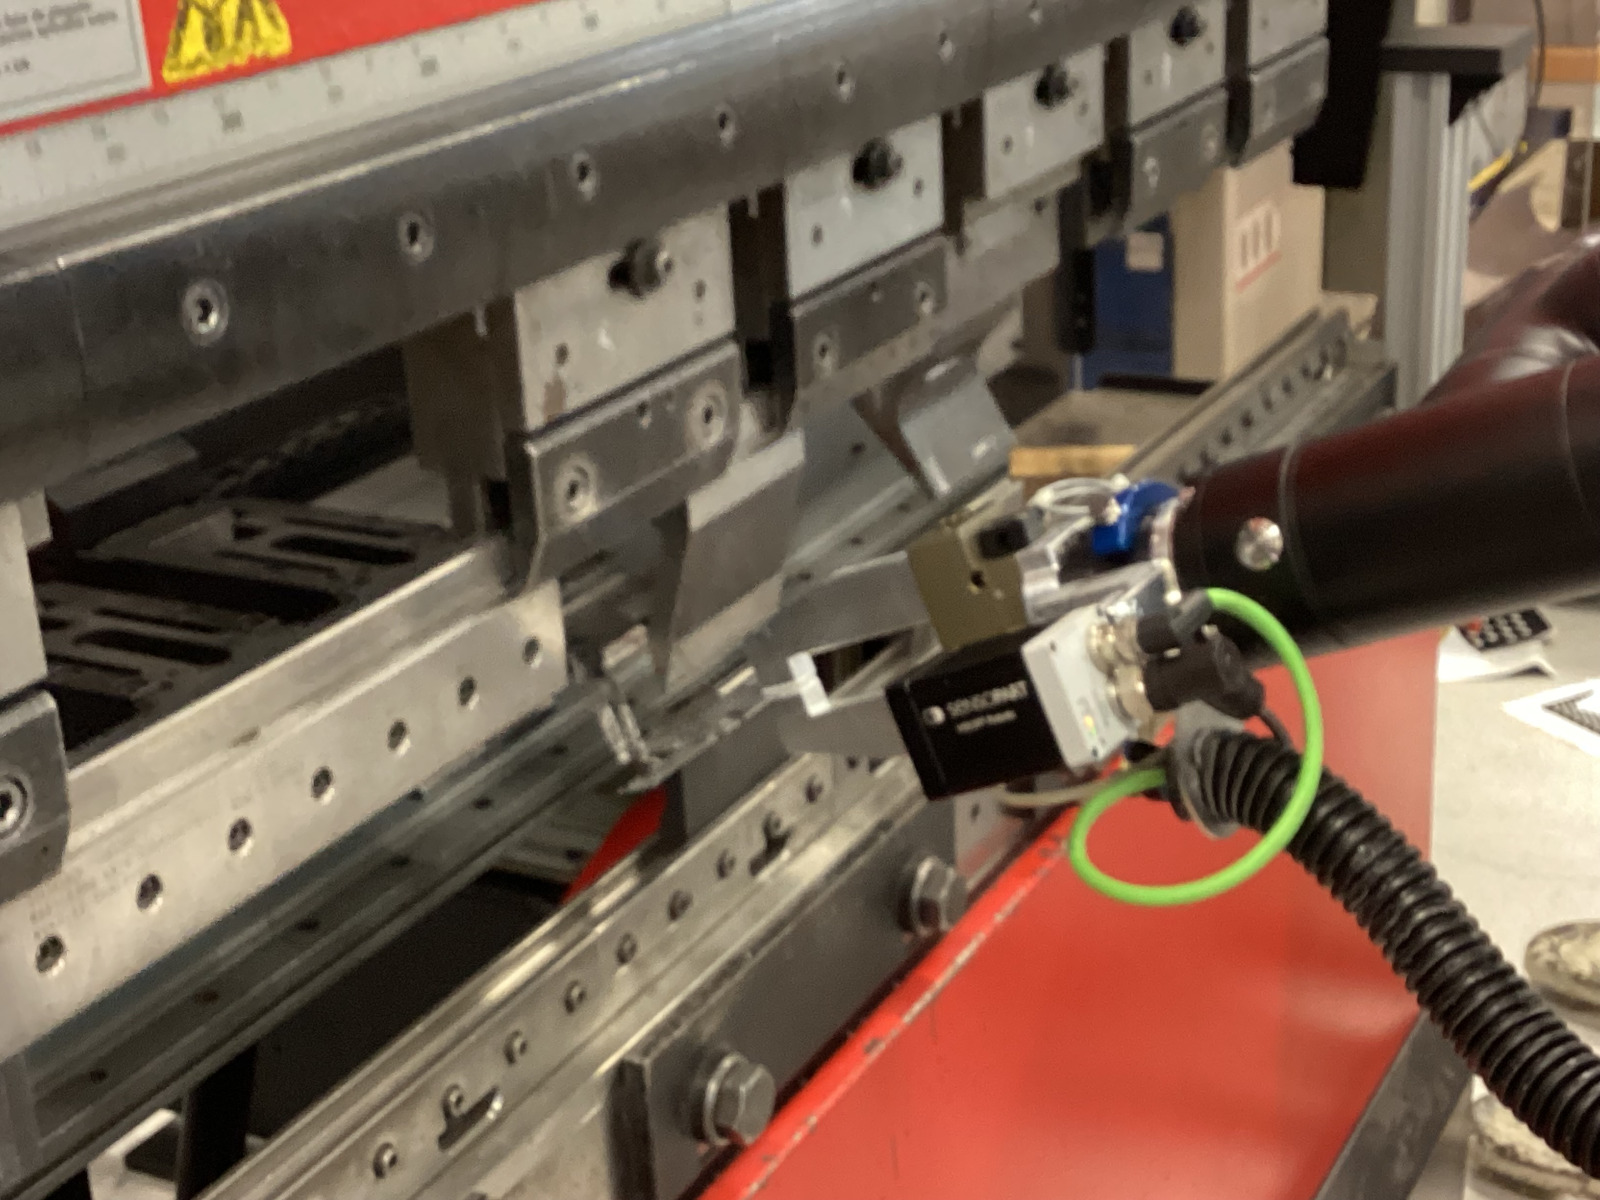
\includegraphics[width=\textwidth]{figures/bending/bending2-002.png}
        \caption{take away the bent sheet}
        \label{subfig:bending2-after}
    \end{subfigure}\hspace{0.1cm}
    \caption{Bending operation number 2 at bending station 2}
    \label{fig:bending-operation-2}
\end{figure}


Figure \ref{fig:bending-operation-1} shows the transfer of sheet metal part to the first bending station where a 90° bend is performed. The handling robot secures the sheet first. A signal is sent by KR1410 robot to PLC to start bending. The robot opens the gripper as soon as the tool of the bending machine hits the sheet. The sheet is secured by the bending machine and the robot moves to a different pose. From there, the robot moves back to the bent part and grip it. Another signal is sent to PLC to move the tool upwards. Once the tool is clear of the part, robot goes to the inspection camera for angle measurement. Bending machine open height measurement laser sensor is responsible for the timings of the opening and closing of bending machine signals. It helps in making robot work together with the bending machine and avoid any collision.


Figures \ref{fig:bending-operation-2} and \ref{fig:bending-operation-3} shows the bending of part at bending station 2. The process is similar to the first bending. The robot leaves the part during bending and regrip it once the bending is complete. For bending number 3, an inspection is not done, because the bending is done very close to the edge, and the small edge is not measurable by the inspection camera.


\begin{figure}[h]
    \centering
    \begin{subfigure}[b]{0.32\textwidth}
        \centering
        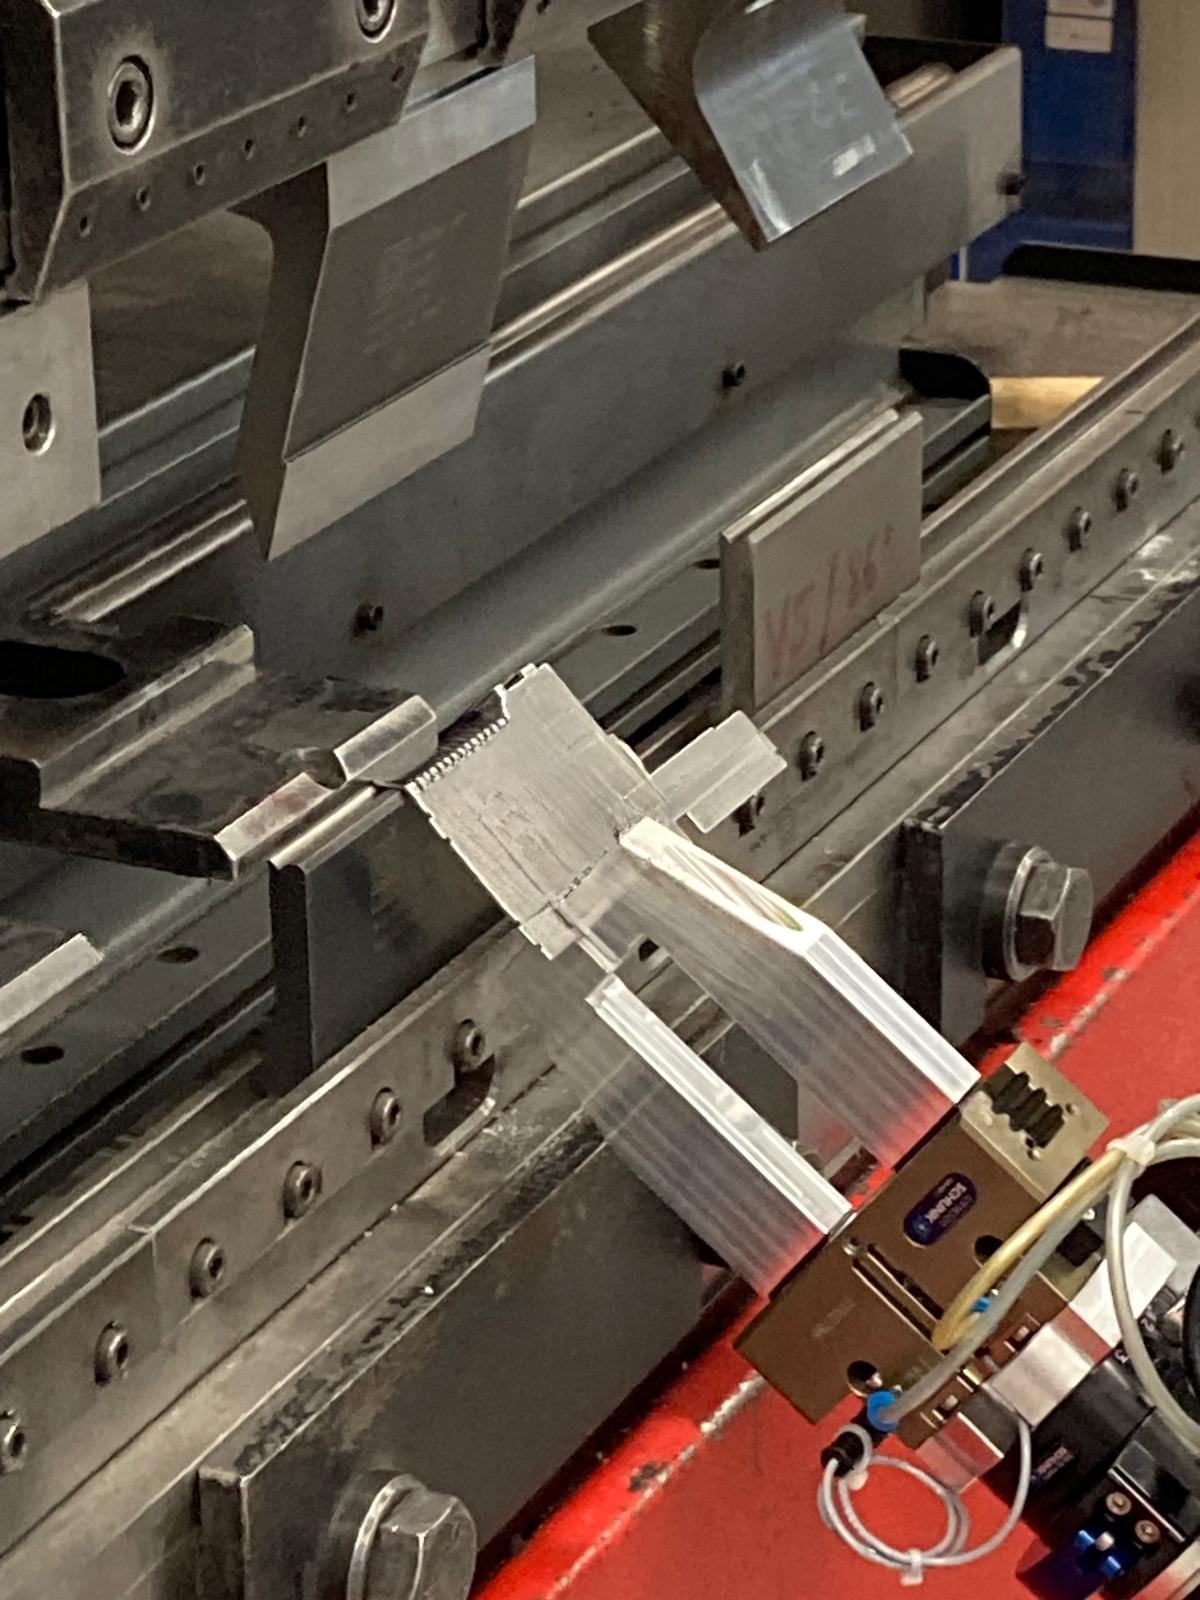
\includegraphics[width=\textwidth]{figures/bending/bending3-001.png}
        \caption{Go to bending station 2}
        \label{subfig:bending3-before}
    \end{subfigure}\hspace{0.1cm}
    \begin{subfigure}[b]{0.32\textwidth}
        \centering
        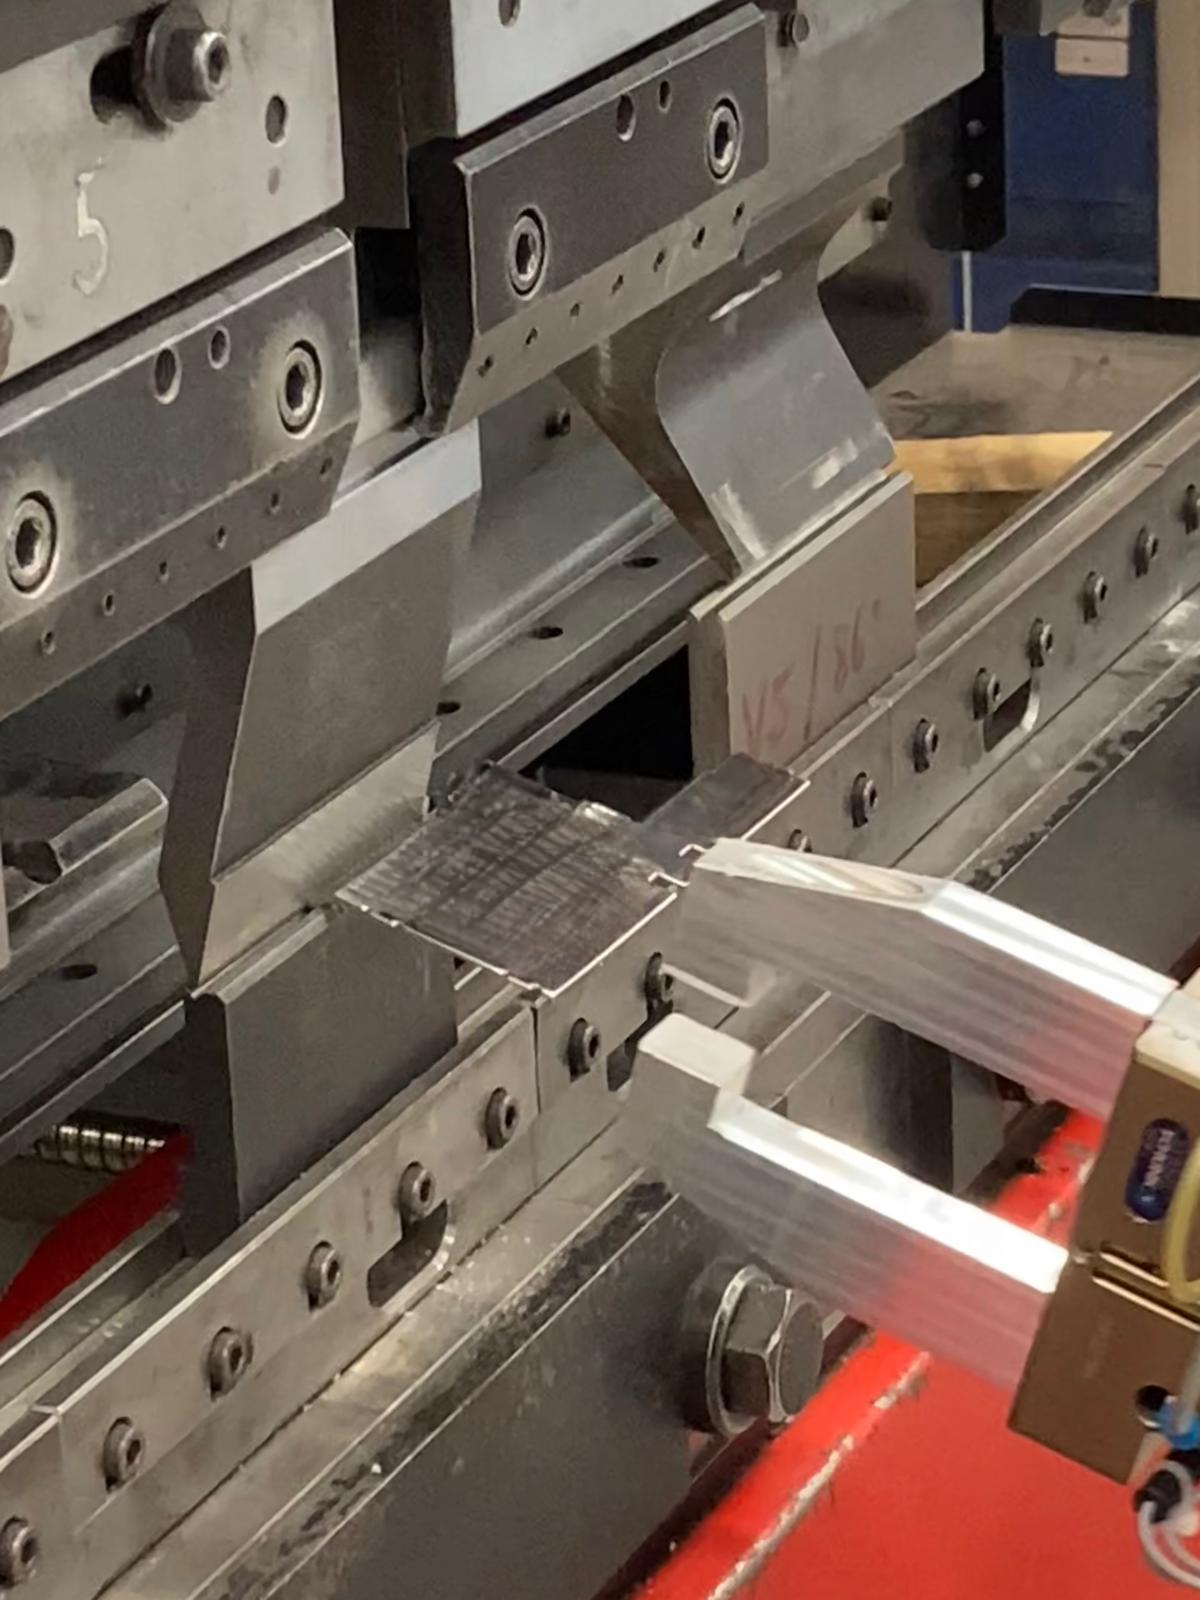
\includegraphics[width=\textwidth]{figures/bending/bending3-002.png}
        \caption{bend the sheet metal part}
        \label{subfig:bending3}
    \end{subfigure}\hspace{0.1cm}
    \begin{subfigure}[b]{0.32\textwidth}
        \centering
        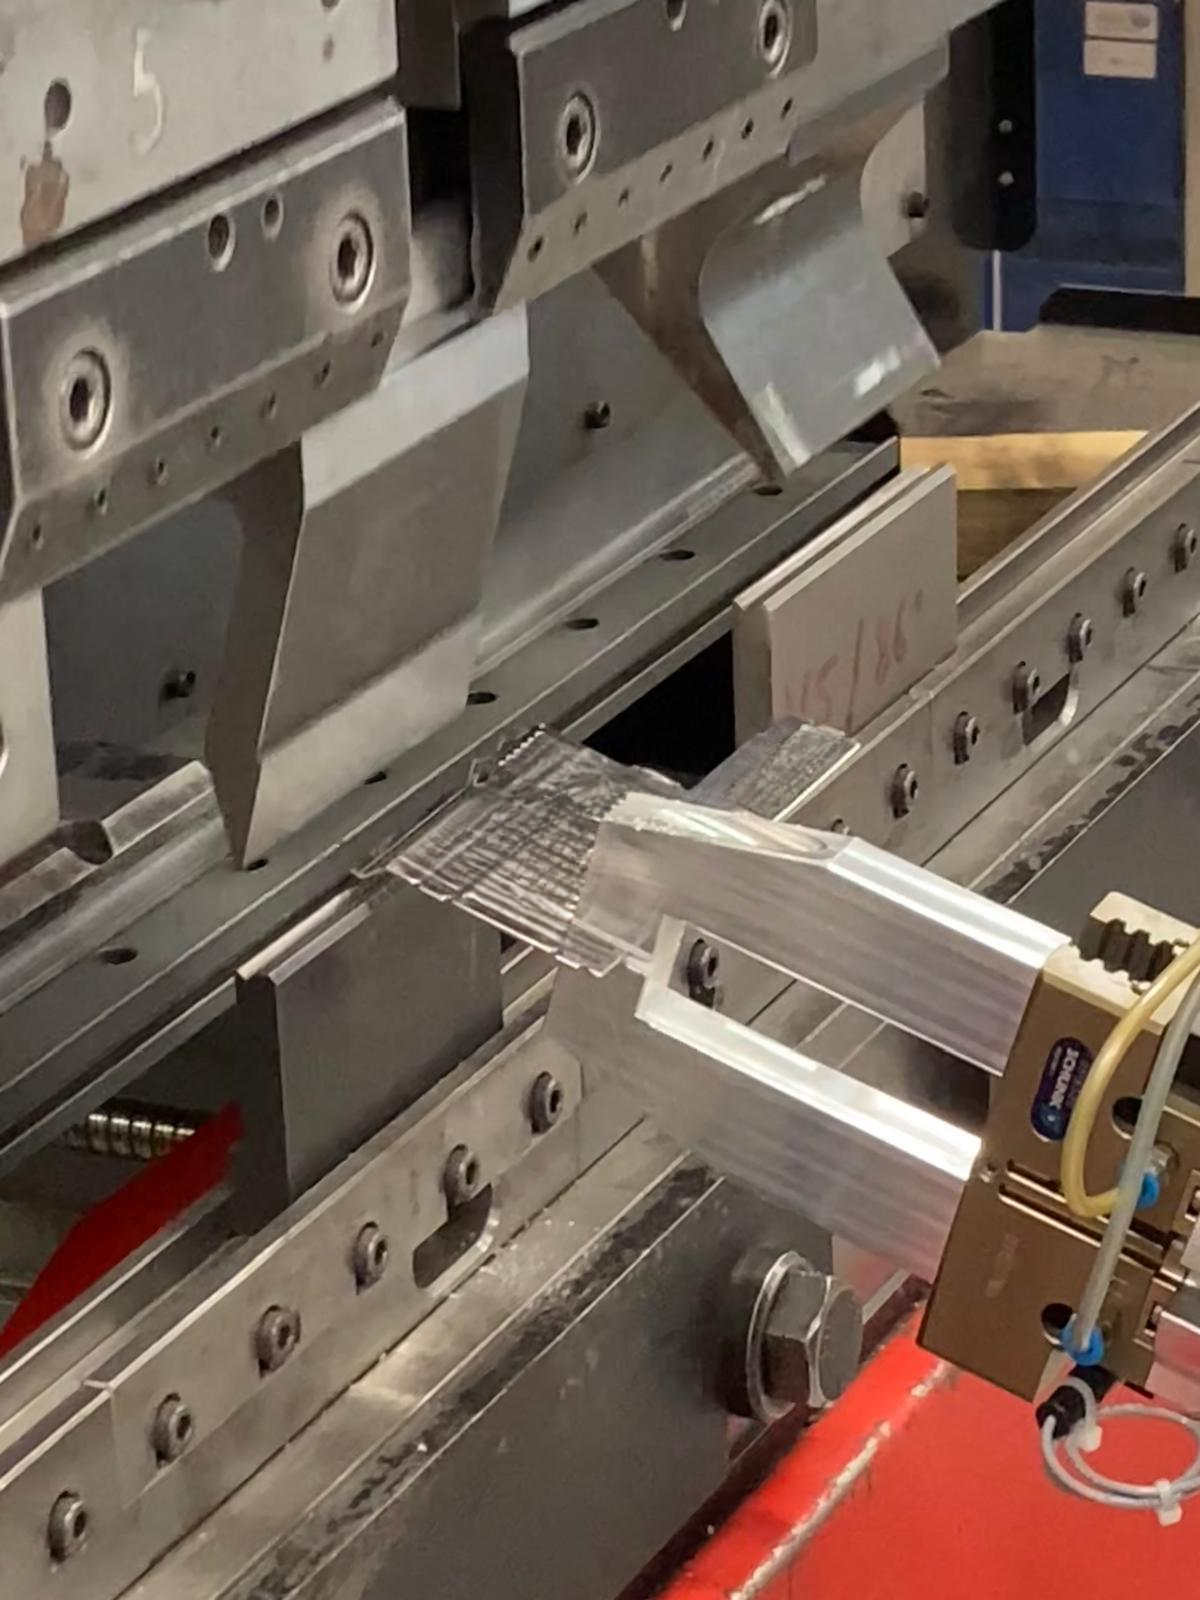
\includegraphics[width=\textwidth]{figures/bending/bending3-003.png}
        \caption{take away the bent sheet}
        \label{subfig:bending3-after}
    \end{subfigure}\hspace{0.1cm}
    \caption{Bending operation number 3 at bending station 2}
    \label{fig:bending-operation-3}
\end{figure}

\begin{figure}[h]
    \centering
    \begin{subfigure}[b]{0.32\textwidth}
        \centering
        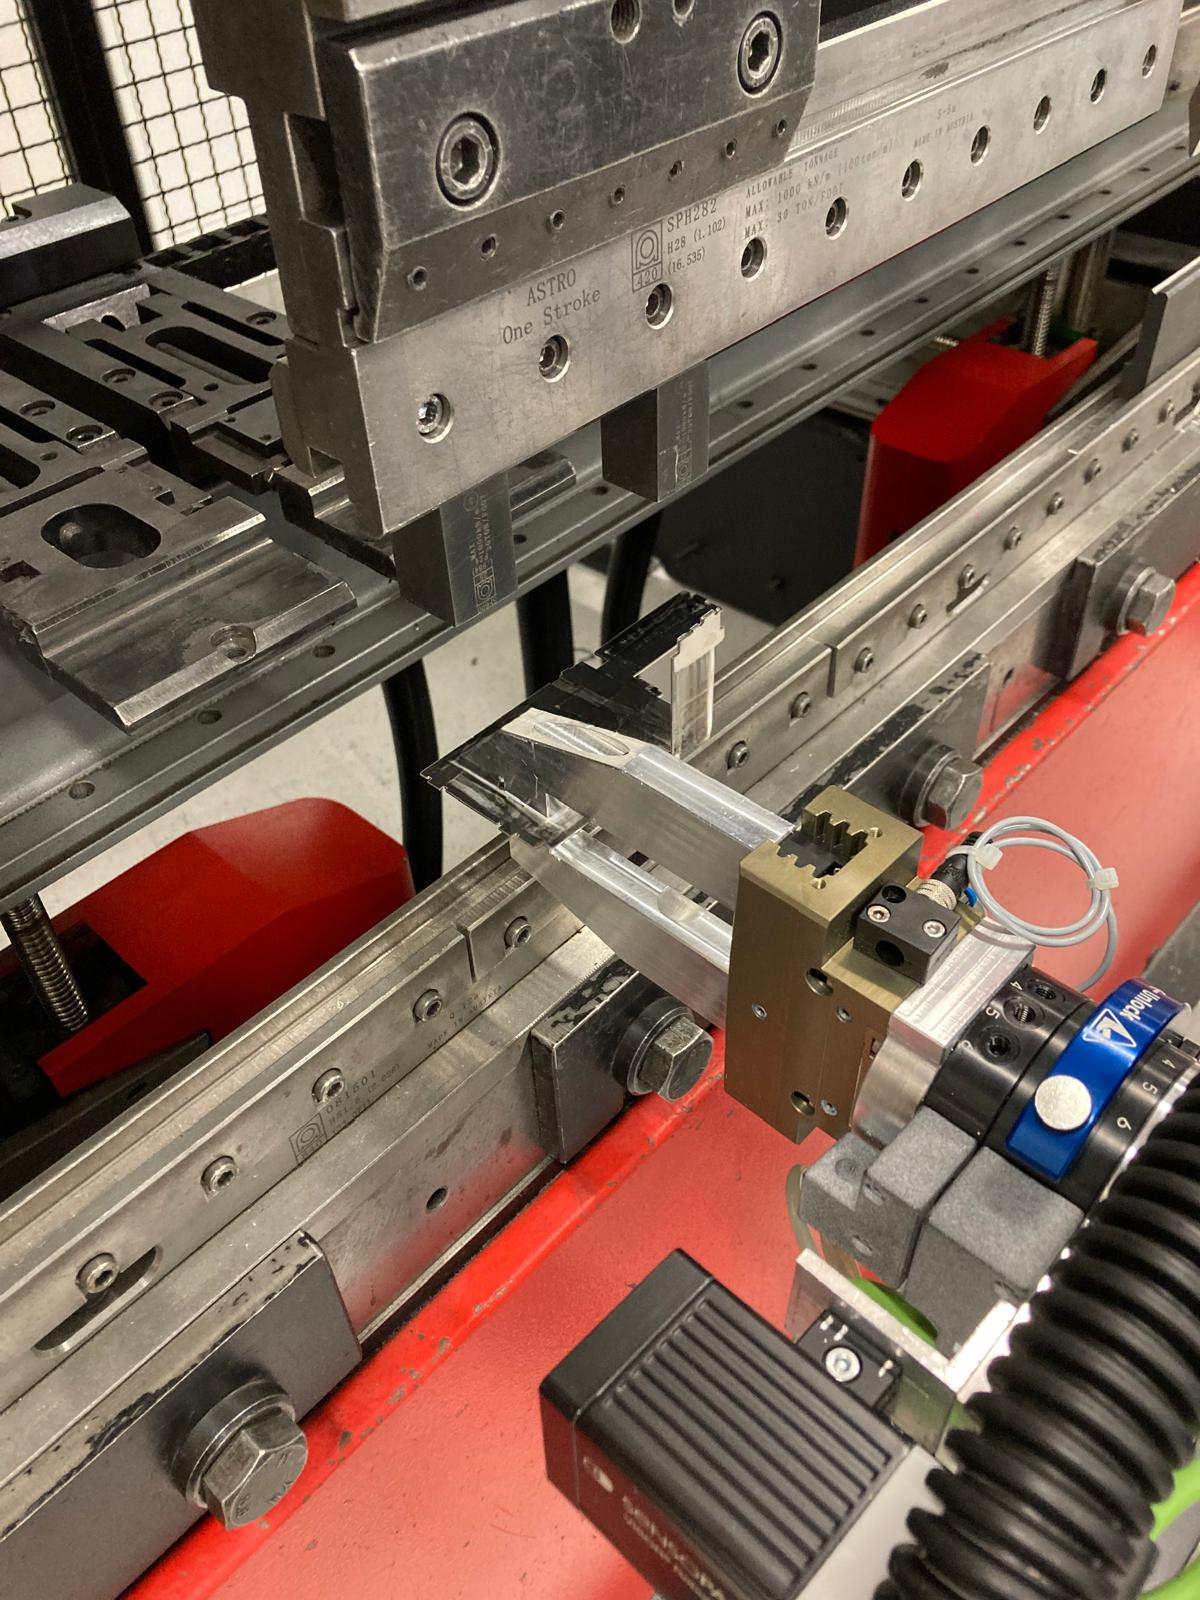
\includegraphics[width=\textwidth]{figures/bending/bending4-001.png}
        \caption{Go to bending station 3}
        \label{subfig:bending4-before}
    \end{subfigure}\hspace{0.1cm}
    \begin{subfigure}[b]{0.32\textwidth}
        \centering
        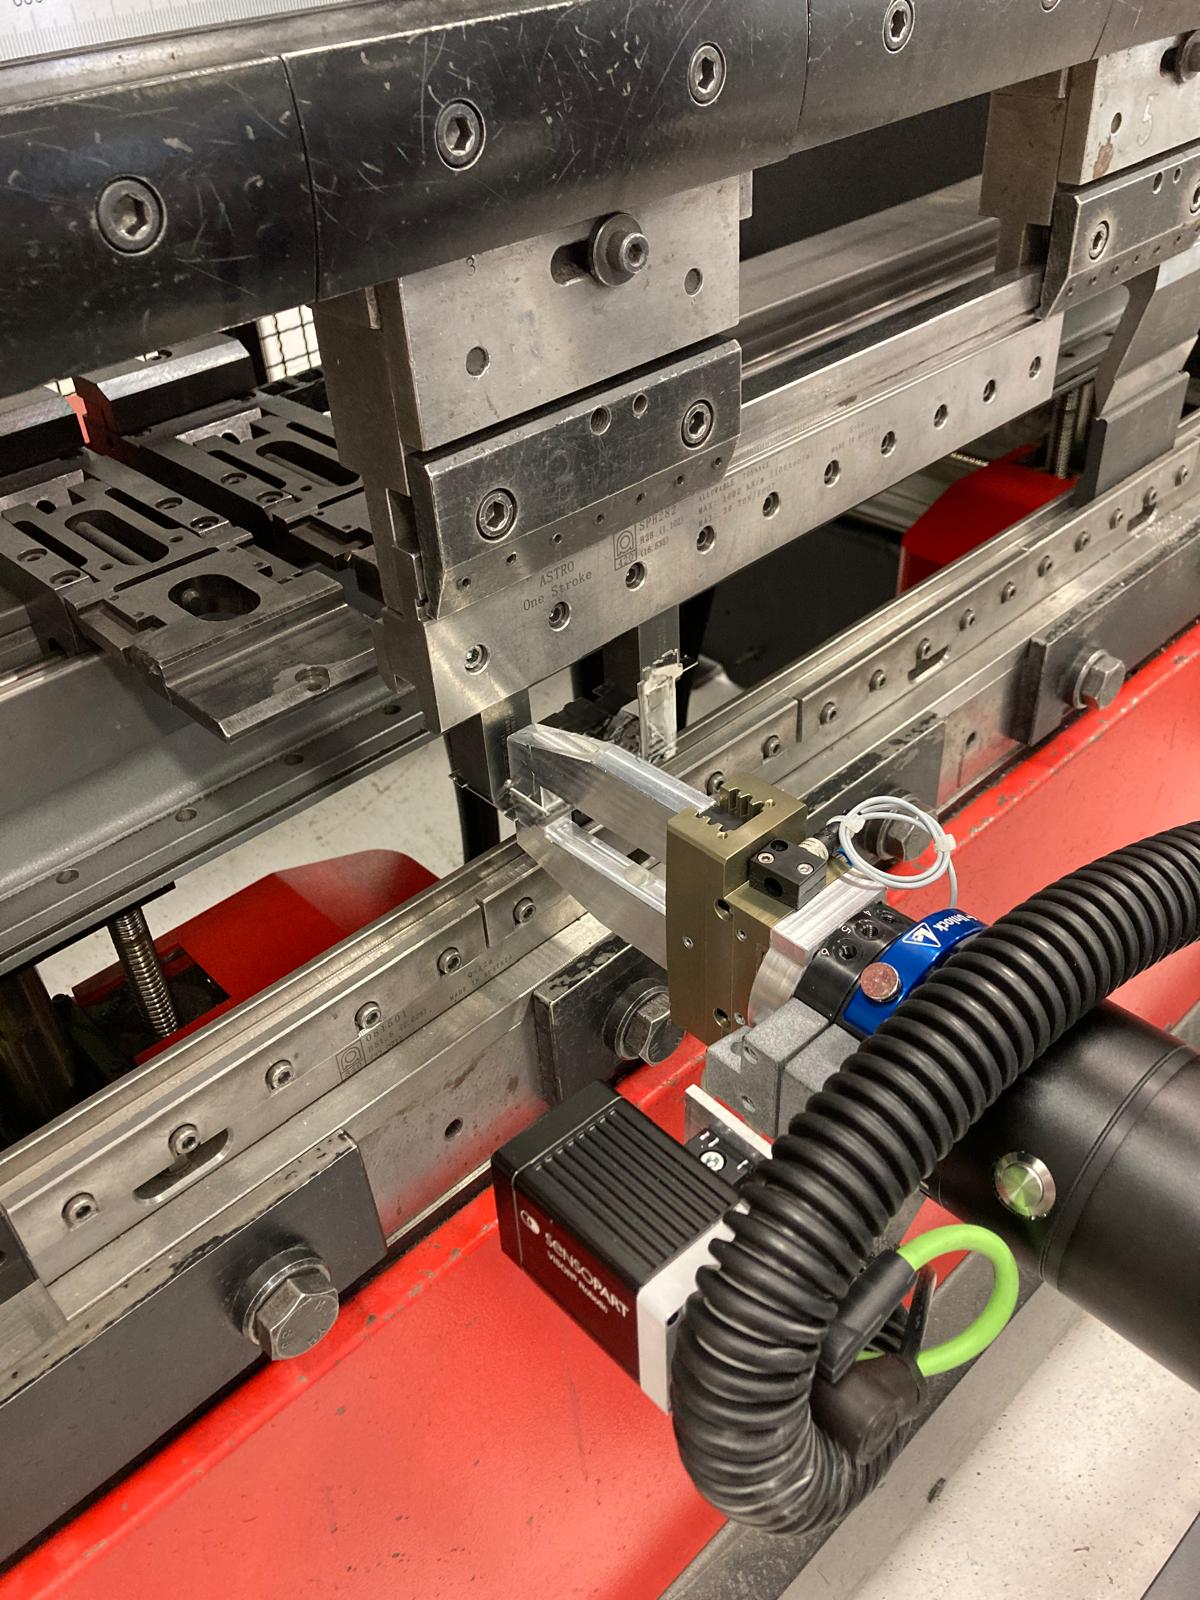
\includegraphics[width=\textwidth]{figures/bending/bending4-002.png}
        \caption{bend the sheet metal part}
        \label{subfig:bending4}
    \end{subfigure}\hspace{0.1cm}
    \begin{subfigure}[b]{0.32\textwidth}
        \centering
        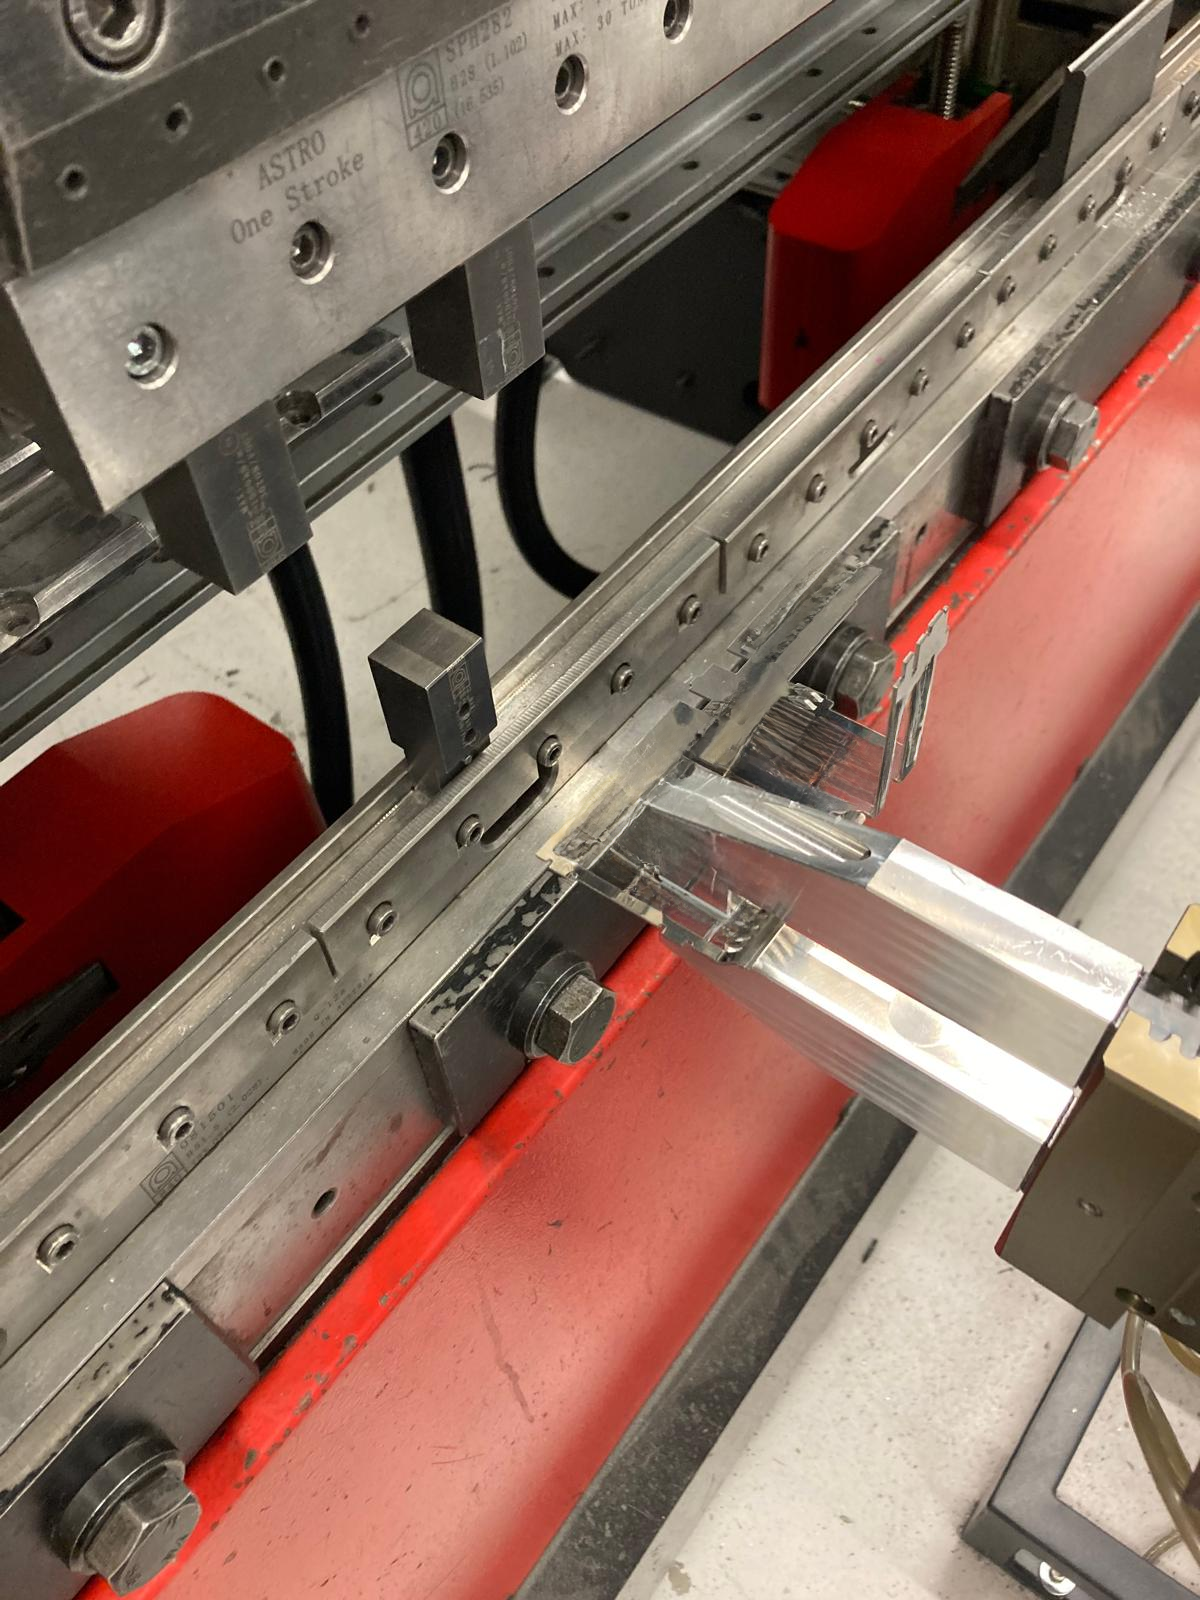
\includegraphics[width=\textwidth]{figures/bending/bending4-003.png}
        \caption{take away the bent sheet}
        \label{subfig:bending4-after}
    \end{subfigure}\hspace{0.1cm}
    \caption{Bending operation number 4 at bending station 3}
    \label{fig:bending-operation-4}
\end{figure}


Figure \ref{fig:bending-operation-4} shows the bending opertion number 4. Since the tool and die are only used for pressing the sheet to flatten it, the robotic gripper doesn't have to open the gripper during bending. Once the sheet is pressed for a specific duration, tool moves up and the robot takes the part out.  Again the inspection is not done, because there is no warping of sheet in this bending operation.


\begin{figure}[h]
    \centering
    \begin{subfigure}[b]{0.32\textwidth}
        \centering
        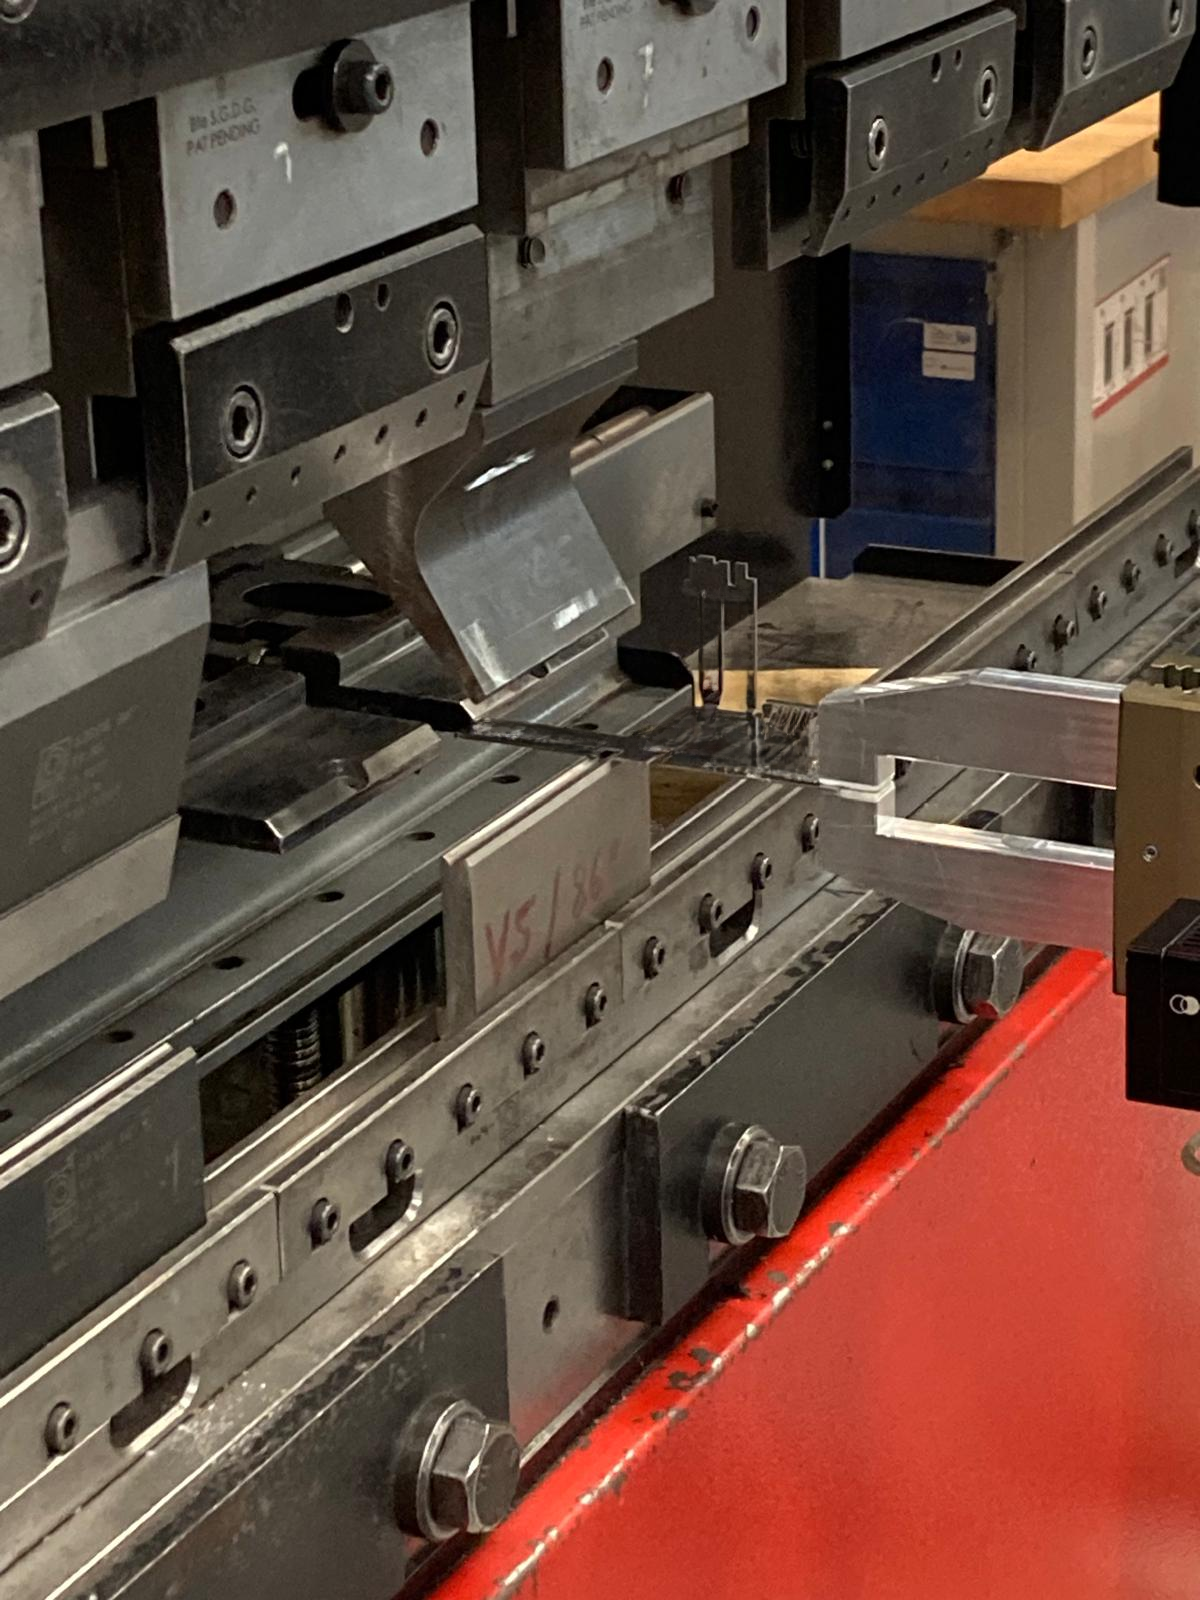
\includegraphics[width=\textwidth]{figures/bending/bending5-001.png}
        \caption{Go to bending station 1}
        \label{subfig:bending5-before}
    \end{subfigure}\hspace{0.1cm}
    \begin{subfigure}[b]{0.32\textwidth}
        \centering
        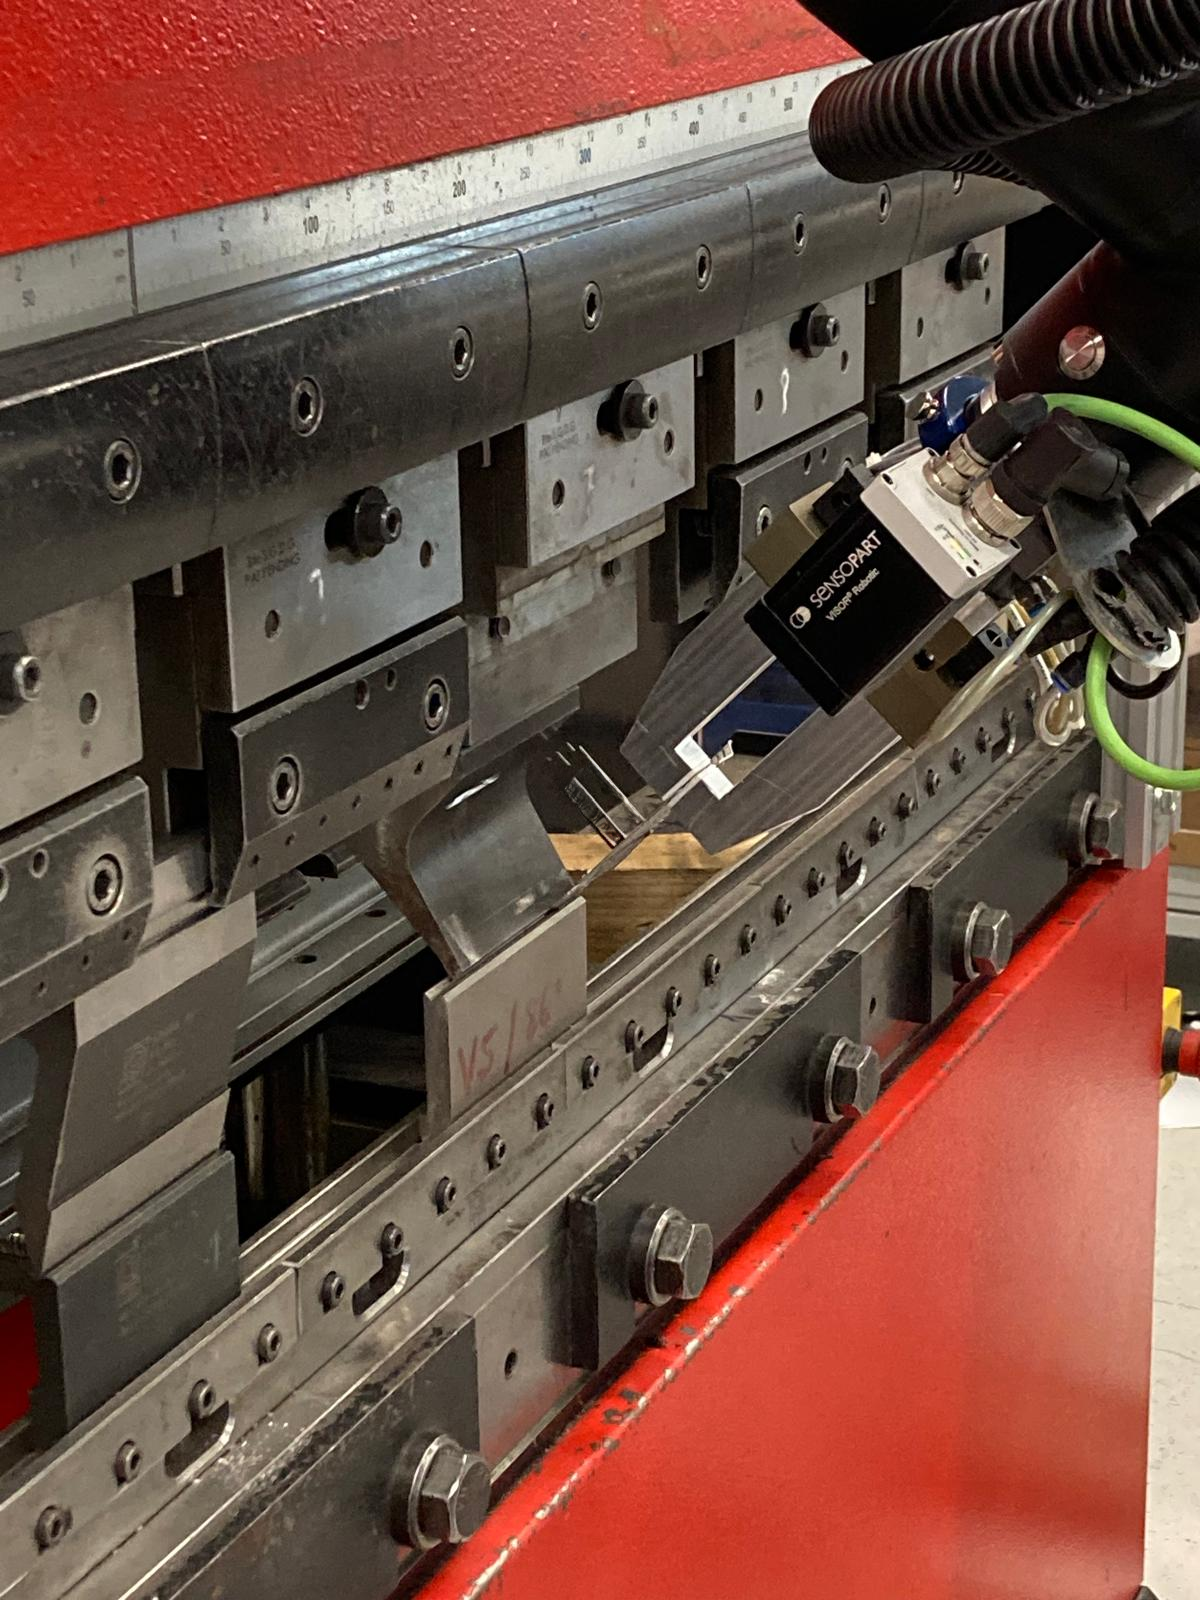
\includegraphics[width=\textwidth]{figures/bending/bending5-002.png}
        \caption{bend the sheet metal part}
        \label{subfig:bending5}
    \end{subfigure}\hspace{0.1cm}
    \begin{subfigure}[b]{0.32\textwidth}
        \centering
        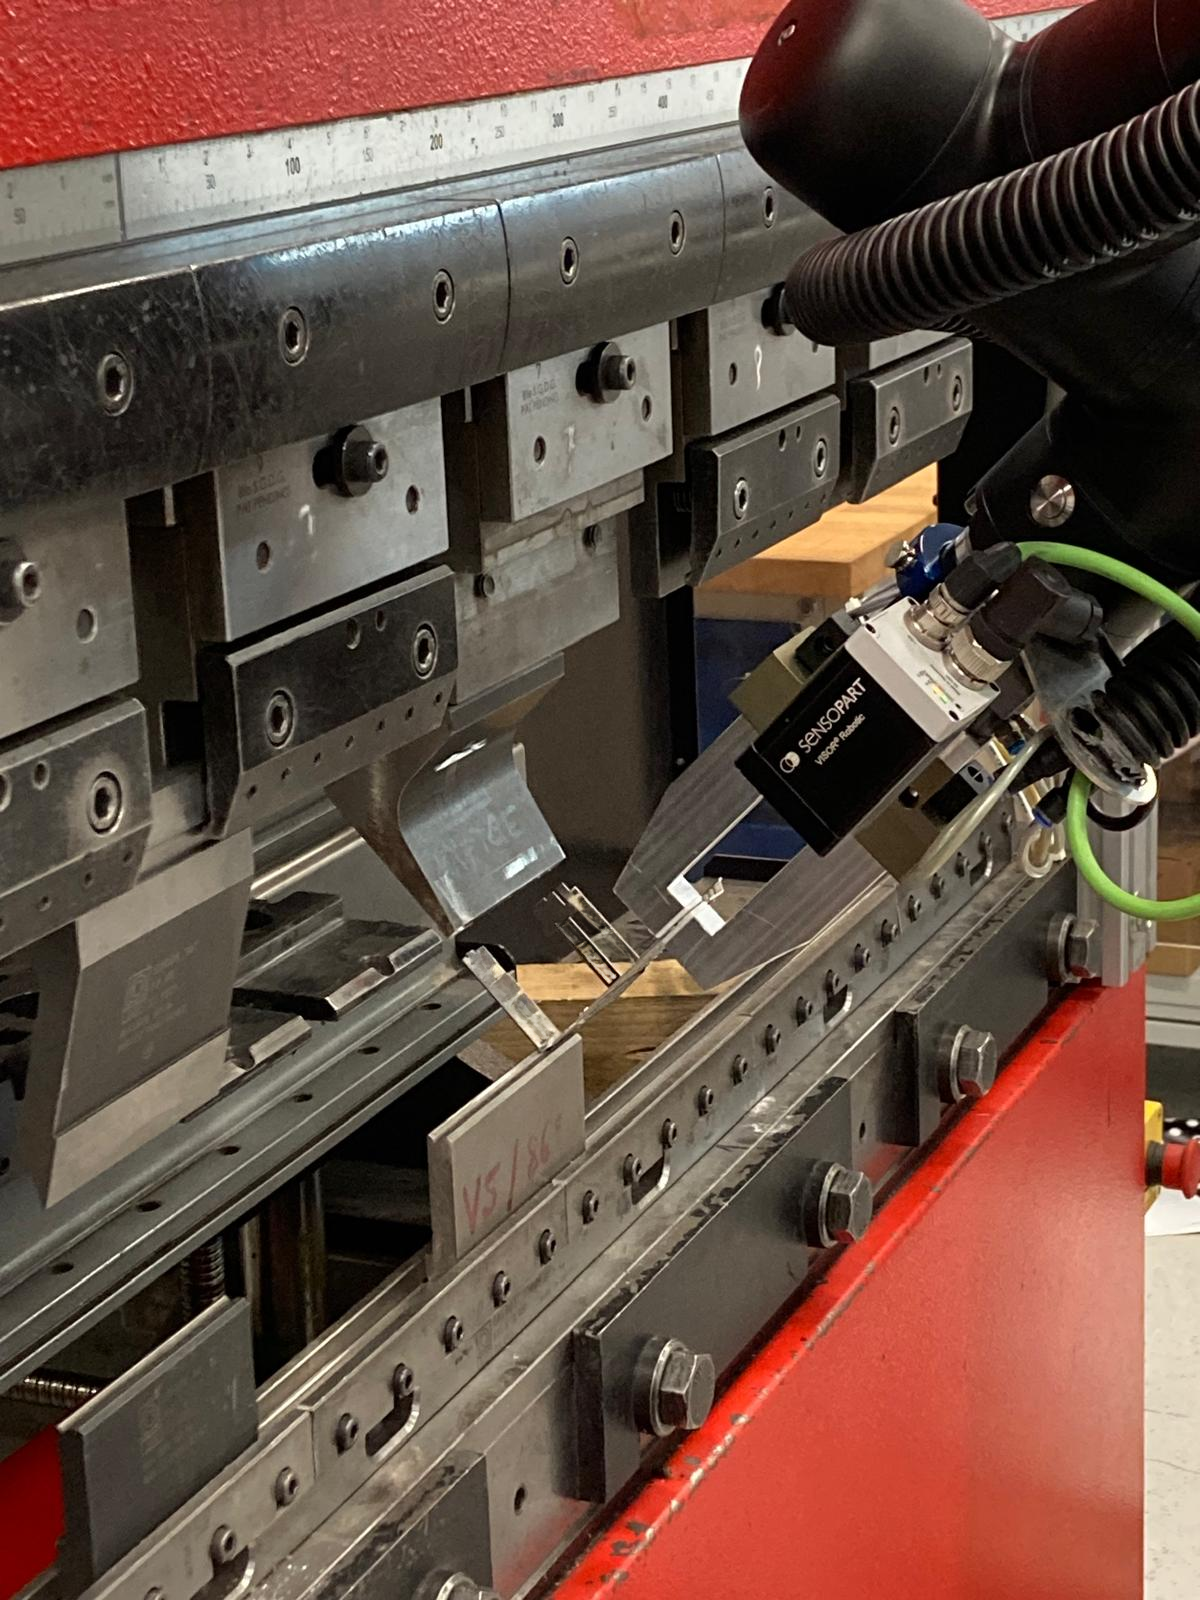
\includegraphics[width=\textwidth]{figures/bending/bending5-003.png}
        \caption{take away the bent sheet}
        \label{subfig:bending5-after}
    \end{subfigure}\hspace{0.1cm}
    \caption{Bending operation number 5 at bending station 1}
    \label{fig:bending-operation-5}
\end{figure}


\begin{figure}[h]
    \centering
    \begin{subfigure}[b]{0.32\textwidth}
        \centering
        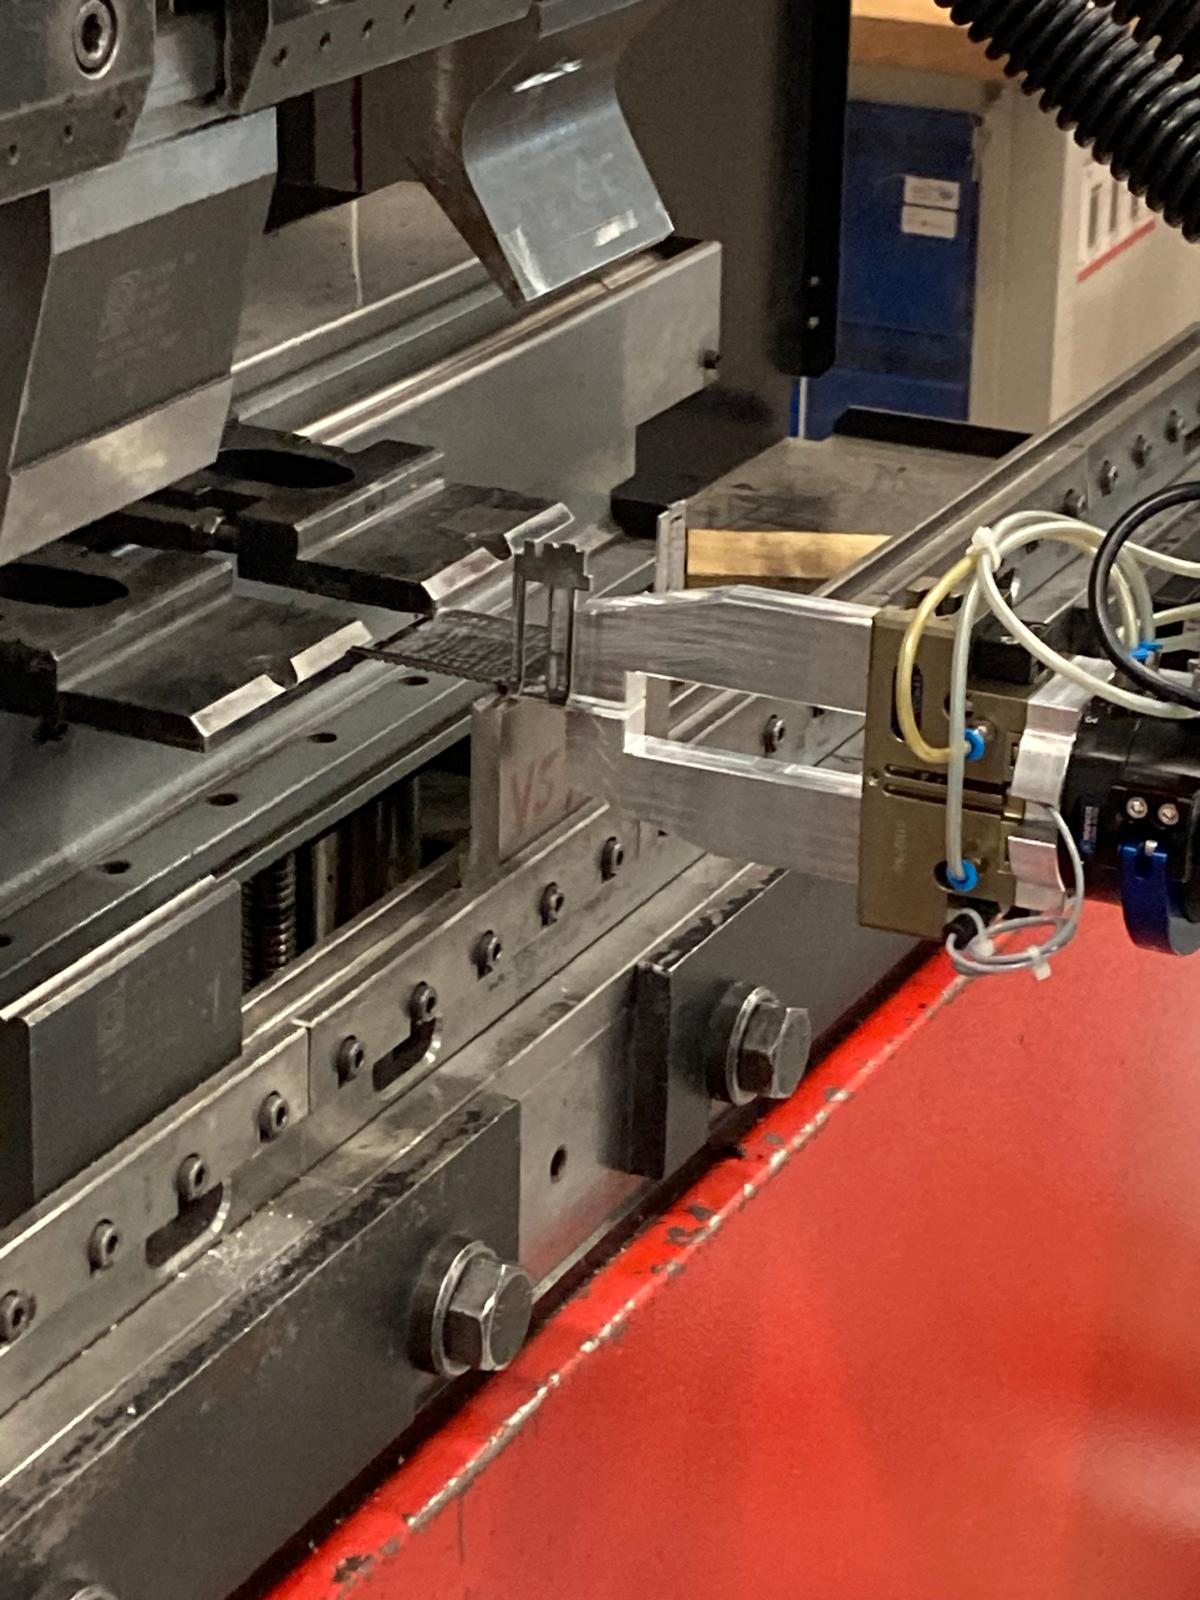
\includegraphics[width=\textwidth]{figures/bending/bending6-001.png}
        \caption{Go to bending station 1}
        \label{subfig:bending6-before}
    \end{subfigure}\hspace{0.1cm}
    \begin{subfigure}[b]{0.32\textwidth}
        \centering
        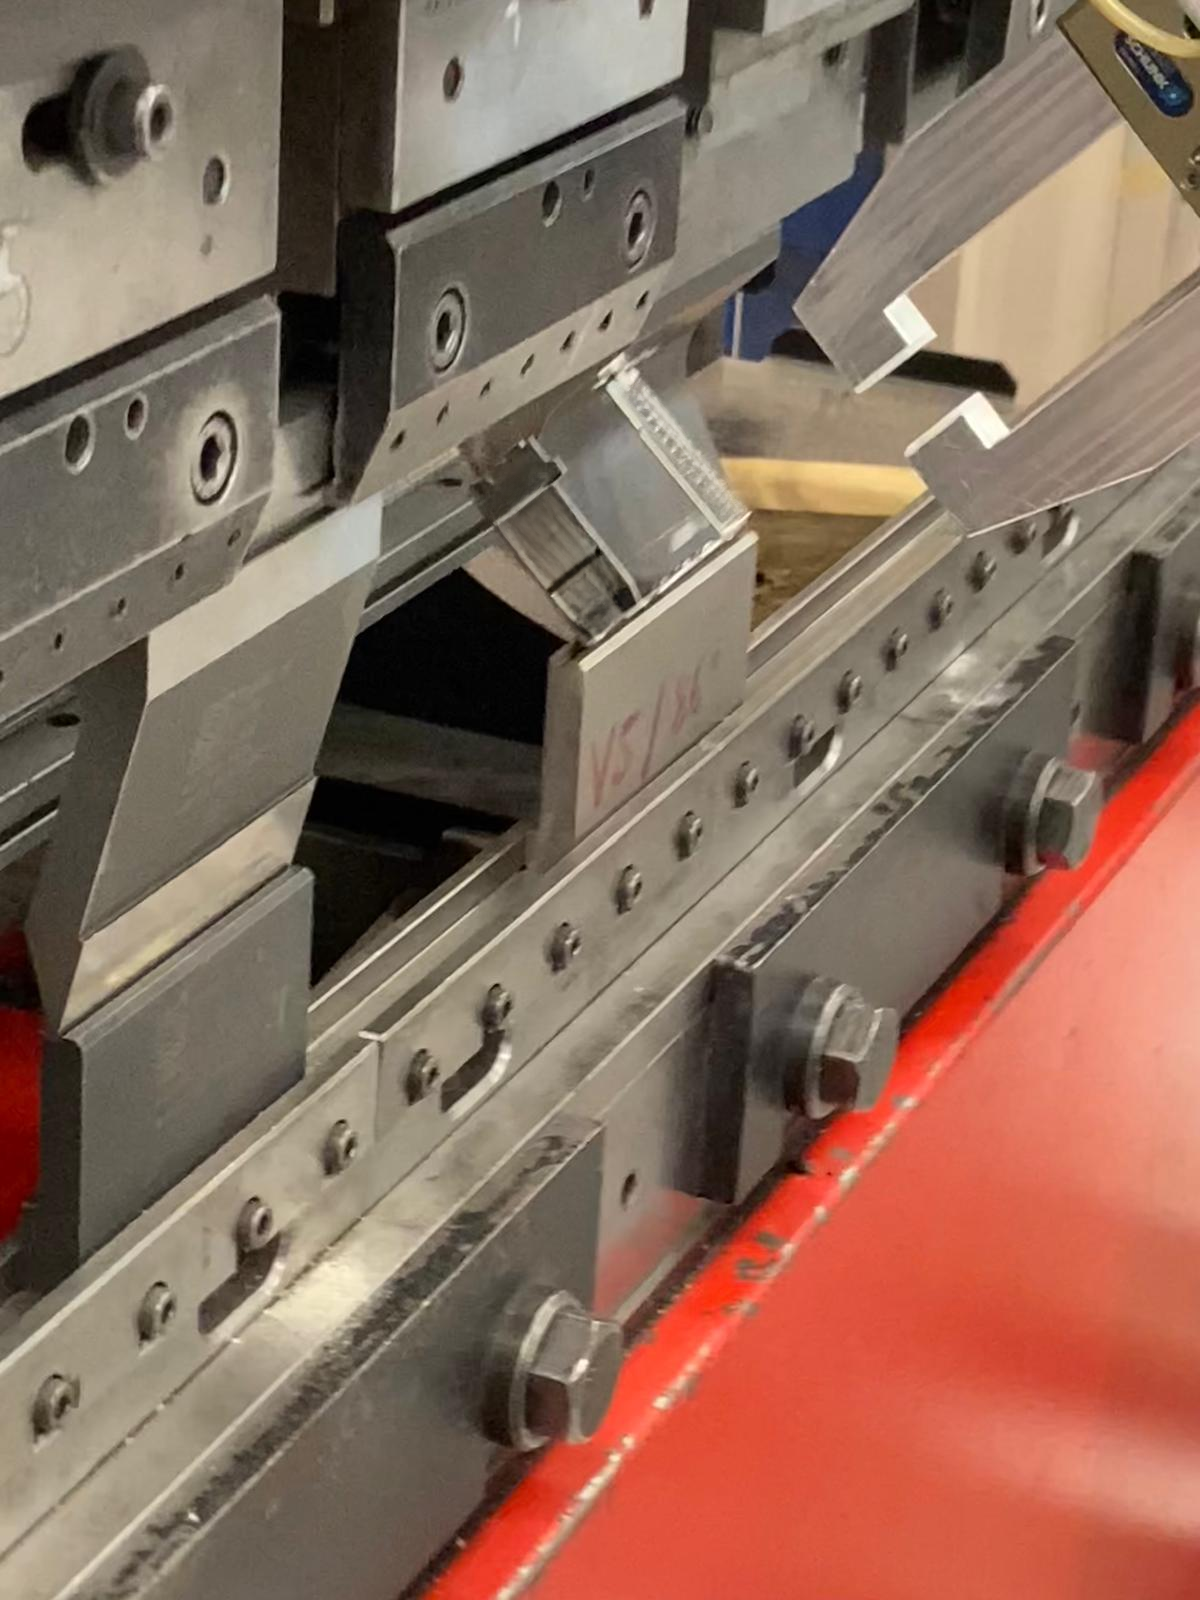
\includegraphics[width=\textwidth]{figures/bending/bending6-003.png}
        \caption{bend the sheet metal part}
        \label{subfig:bending6}
    \end{subfigure}\hspace{0.1cm}
    \begin{subfigure}[b]{0.32\textwidth}
        \centering
        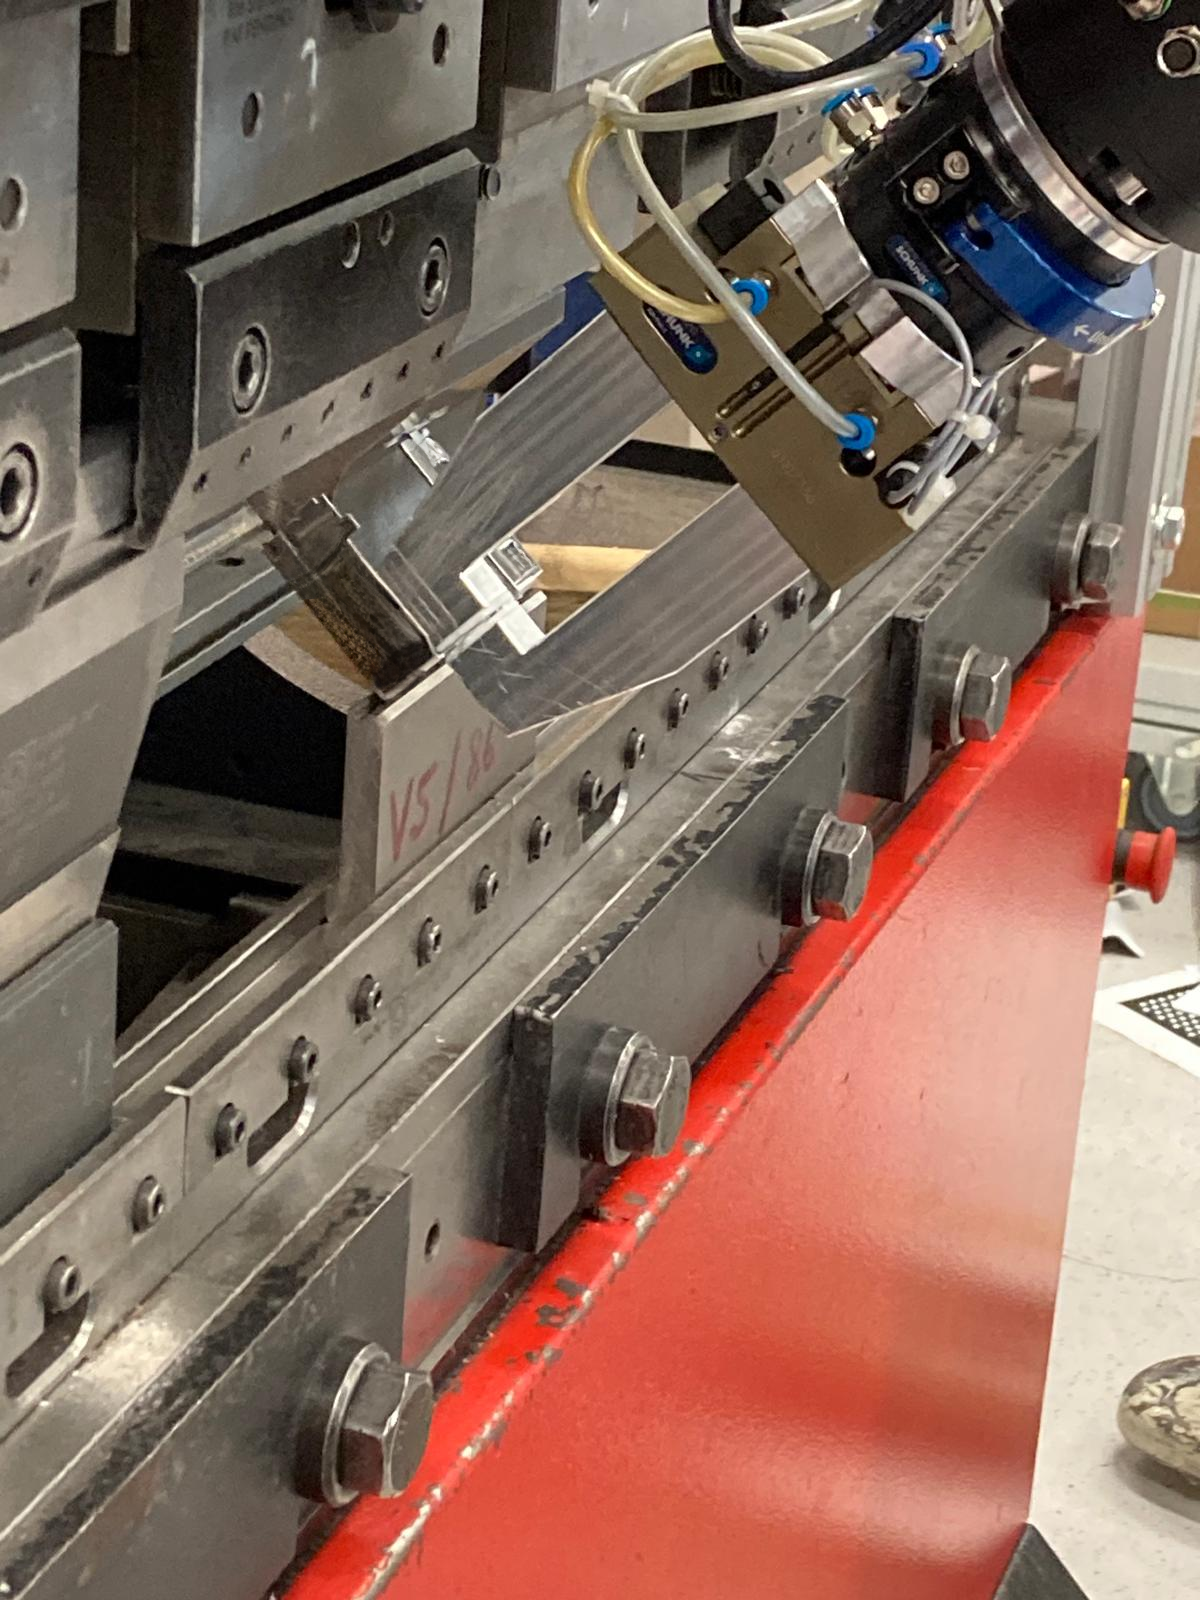
\includegraphics[width=\textwidth]{figures/bending/bending6-002.png}
        \caption{take away the bent sheet}
        \label{subfig:bending6-after}
    \end{subfigure}\hspace{0.1cm}
    \caption{Bending operation number 6 at bending station 1}
    \label{fig:bending-operation-6}
\end{figure}

Bending operation 5 and 6 are performed at bending station 1 as showing in figures \ref{fig:bending-operation-5} and \ref{fig:bending-operation-6} respectively. The process is similar to bending operation 1 as the robot doesn't hold the part during bending. Inspection is done after both bending operations. If after bending operation 6, the angle measurement is within tolerances, the current bending cycle is termed as successful.
\FloatBarrier  % Force all figures of the first section to be placed before the next section

\subsection{Inspection Setup}
\label{subsec:inspection}

After a bending operation, the sheet is taken to the inspection camera installed on the unloading station.
At this pose, the inspection camera is triggered by the \hyperref[acro:PLC]{PLC} as shown in figure \ref{fig:inspection-setup}. The image is captured, and the results are sent to the PLC.

\begin{figure}[h]
    \centering
    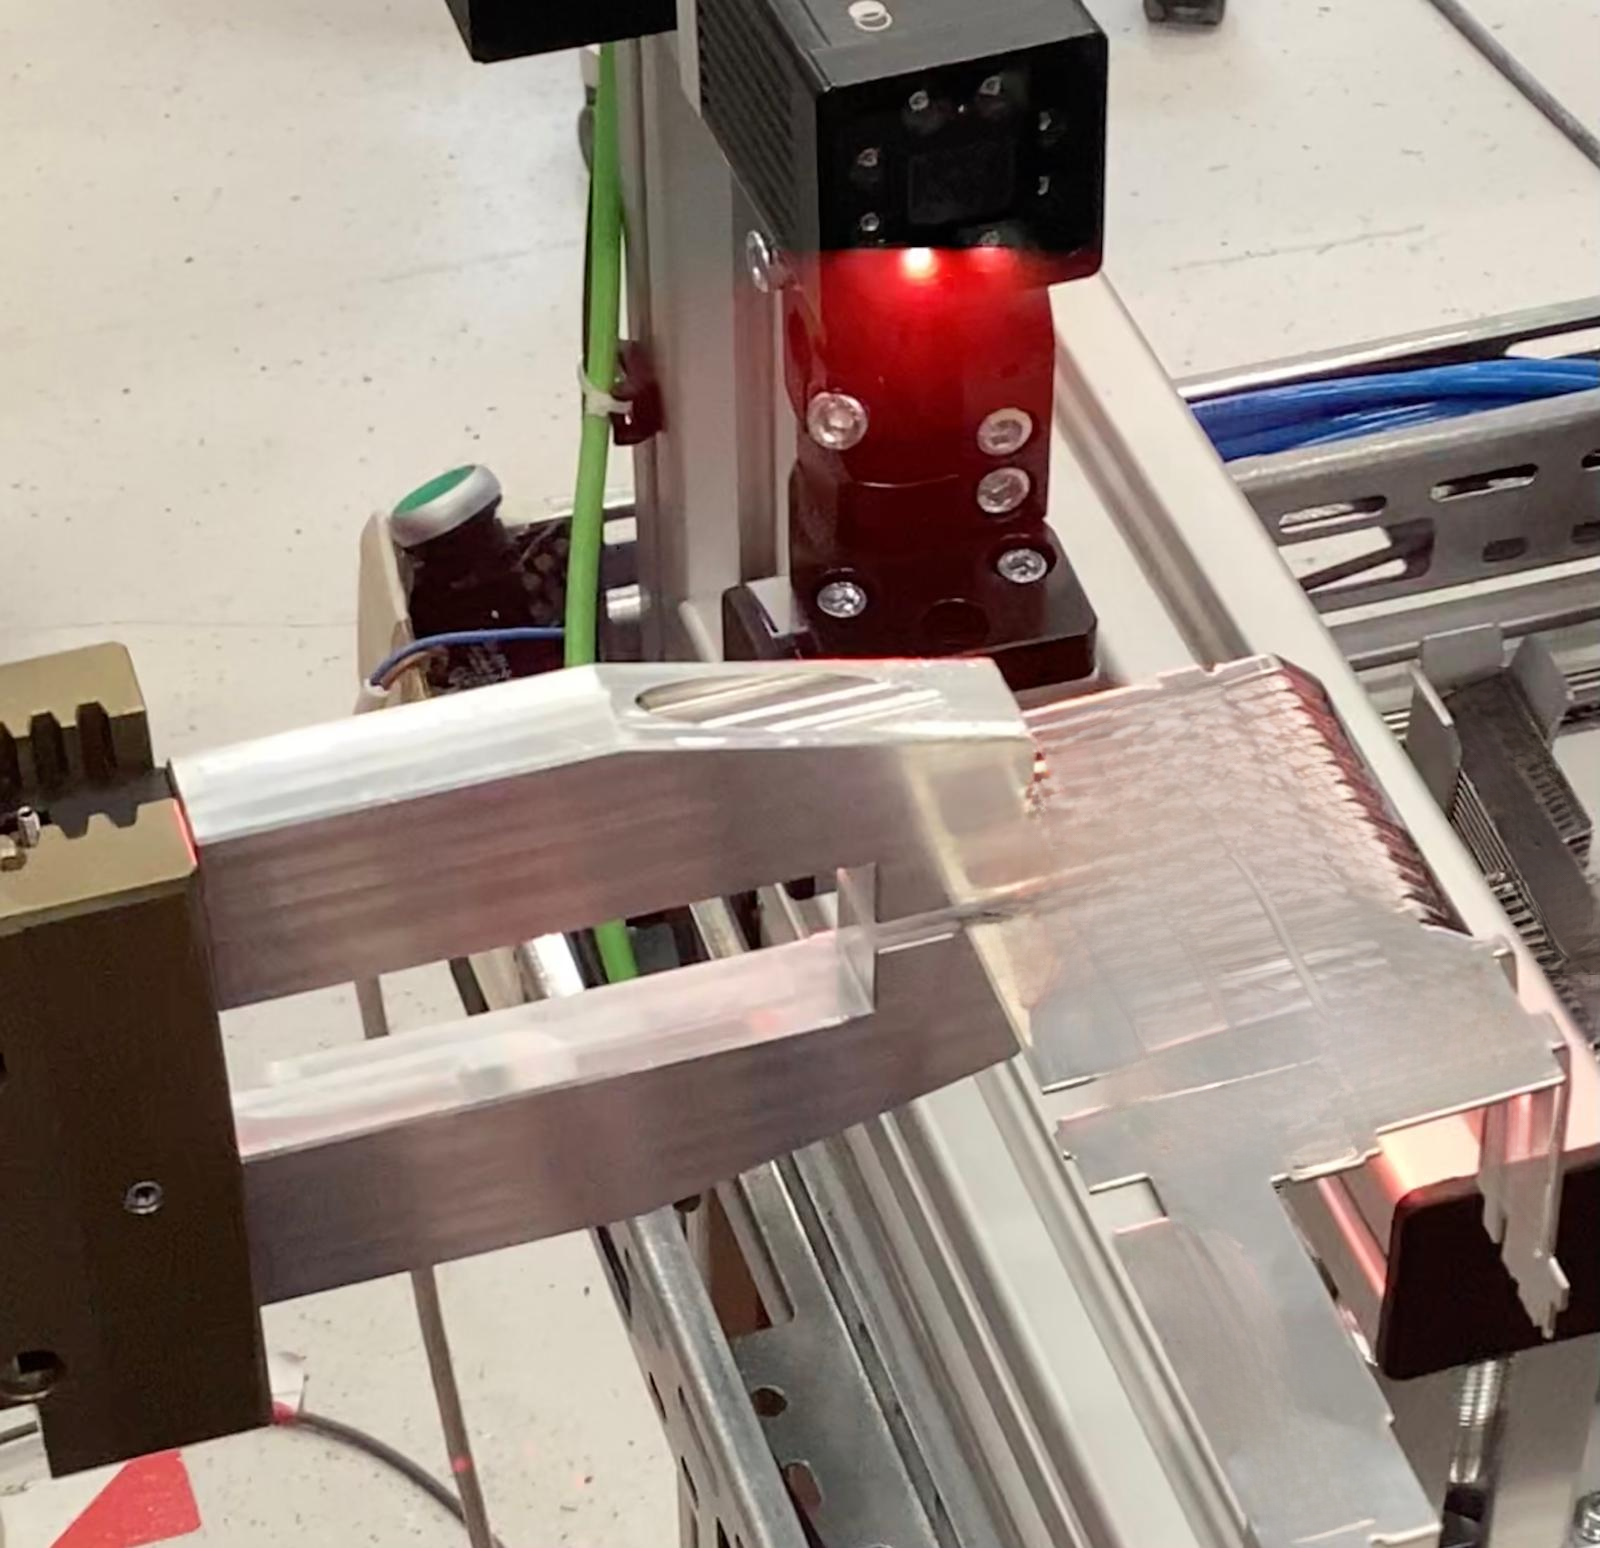
\includegraphics[width=0.6\textwidth]{figures/inspection-setup.png}
    \caption{Robot aligns bent sheet in front of inspection camera}
    \label{fig:inspection-setup}
\end{figure}

The inspection camera measures the bending angle of the sheet metal part. If any discrepancies are detected, the \hyperref[acro:PLC]{PLC} sends feedback to adjust the bending parameters to the bending machine, ensuring continuous improvement in accuracy and quality for the next cycle. These bending parameters are updated by the terminal operating robot.

If the part passes inspection, the \hyperref[acro:KR]{KR1410} proceeds to place it in the storage station. If the part fails inspection, it is automatically transferred to a rejection bin under the unloading station.
\FloatBarrier  % Force all figures of the first section to be placed before the next section

\subsection{Shelf Control}
\label{subsec:shelf-control}

\begin{figure}[h]
    \centering
    \begin{subfigure}[b]{0.32\textwidth}
        \centering
        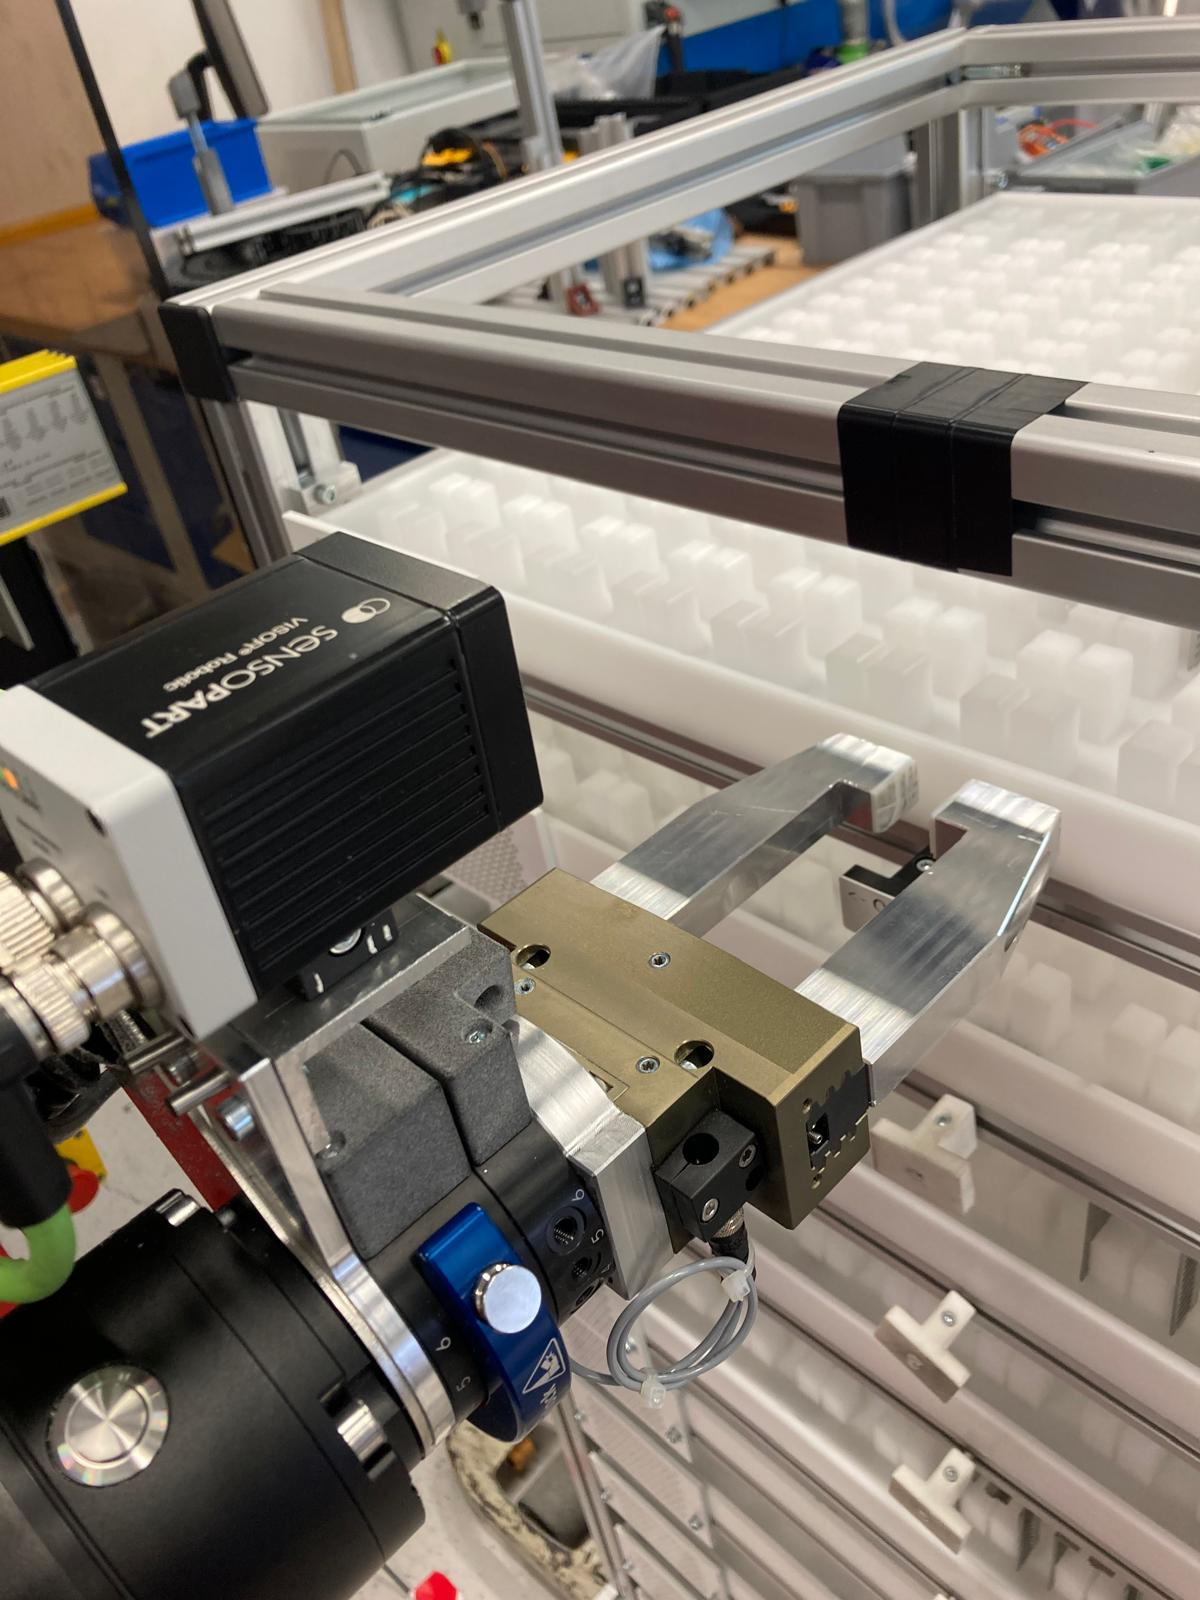
\includegraphics[width=\textwidth]{figures/shelf-control/reach-handle.jpeg}
        \caption{Reach shelf handle}
        \label{subfig:reach-handle}
    \end{subfigure}\hspace{0.1cm}
    \begin{subfigure}[b]{0.32\textwidth}
        \centering
        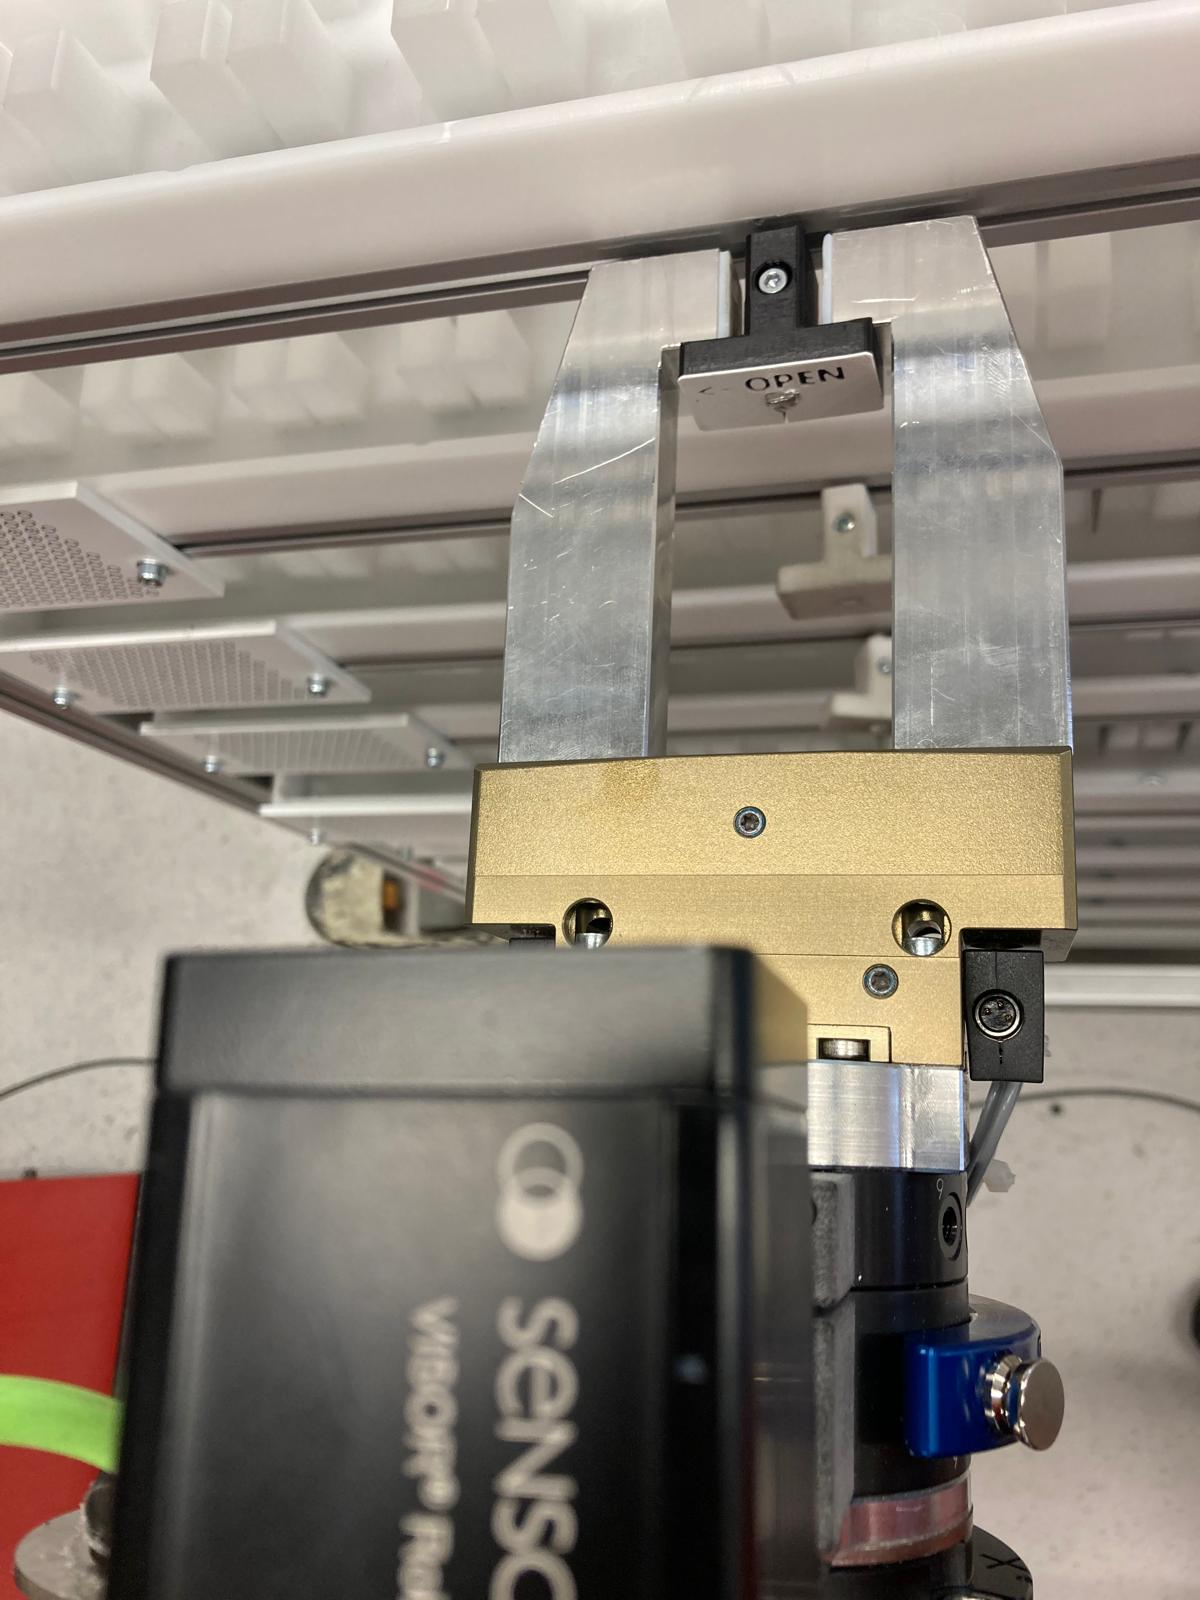
\includegraphics[width=\textwidth]{figures/shelf-control/hold-handle.jpeg}
        \caption{grasp handle with gripper}
        \label{subfig:grasp-handle}
    \end{subfigure}\hspace{0.1cm}
    \vspace{1cm}
    \begin{subfigure}[b]{0.32\textwidth}
        \centering
        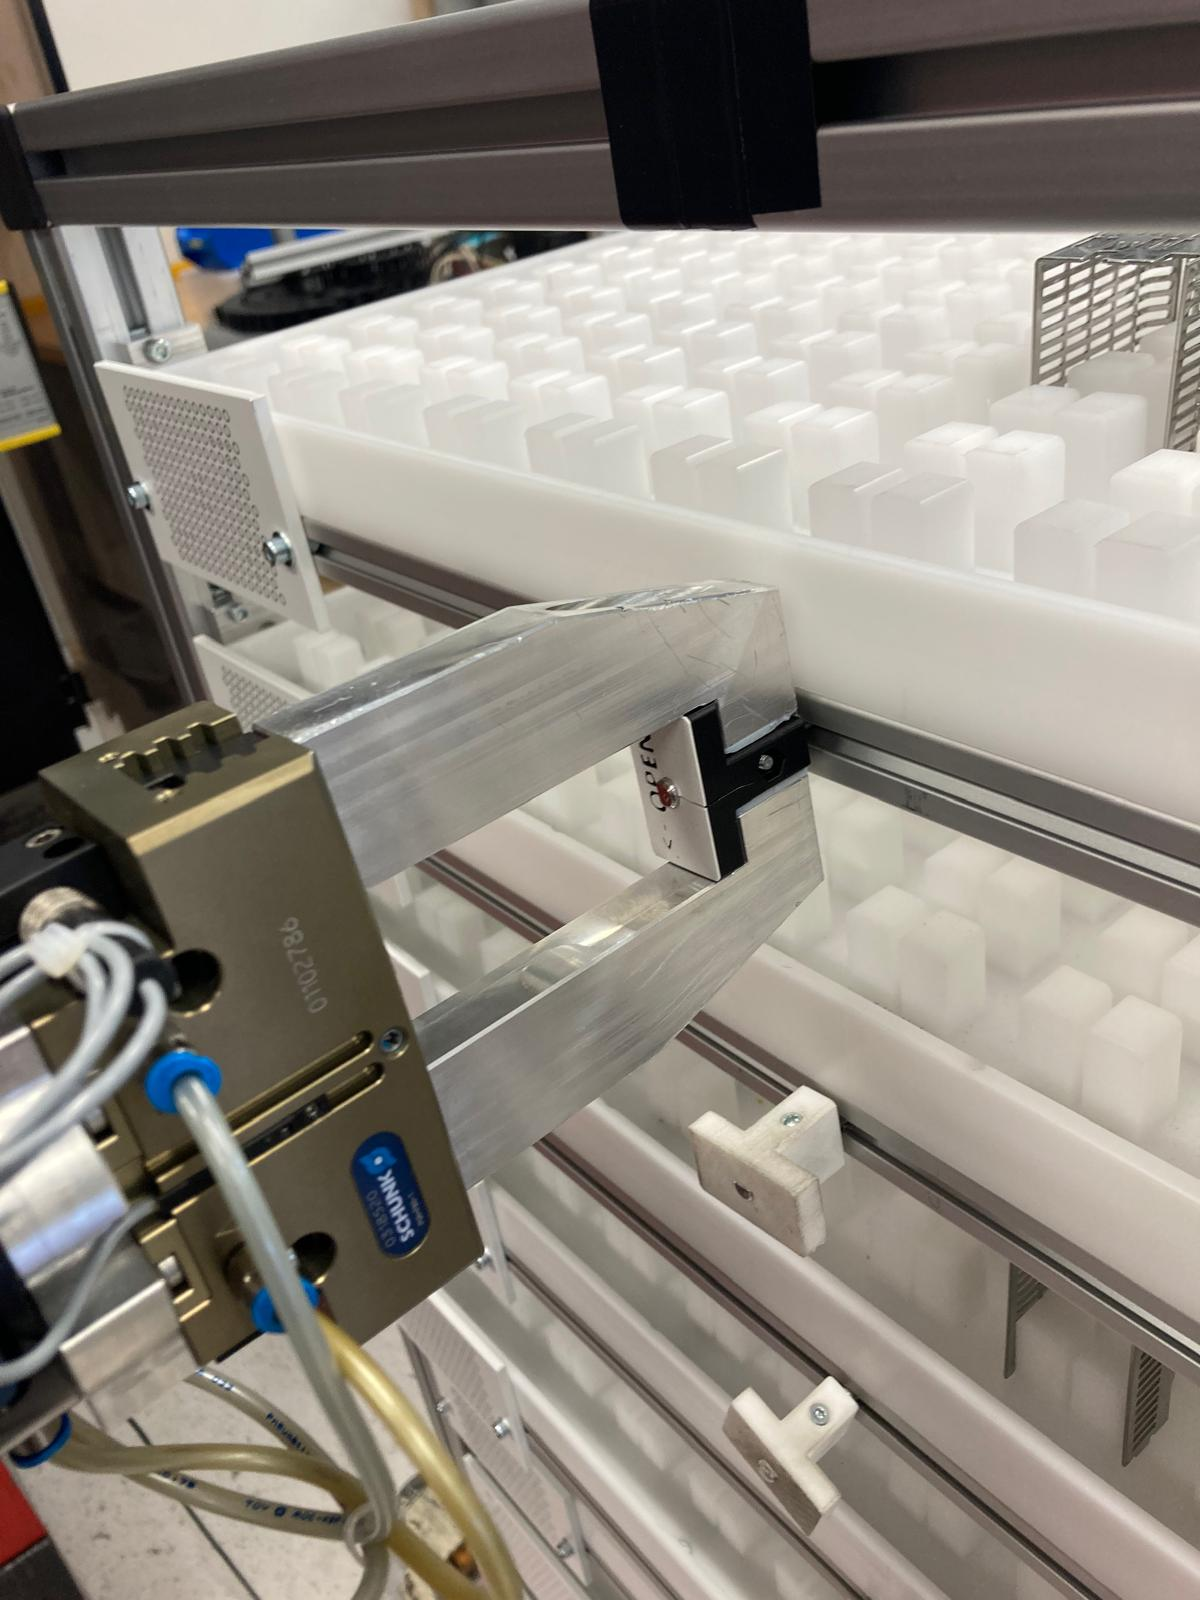
\includegraphics[width=\textwidth]{figures/shelf-control/open-handle.jpeg}
        \caption{Turn handle 100\textdegree{} to open drawer}
        \vspace{-0.45cm}
        \label{subfig:turn-open}
    \end{subfigure}\hspace{0.1cm}
    \begin{subfigure}[b]{0.32\textwidth}
        \centering
        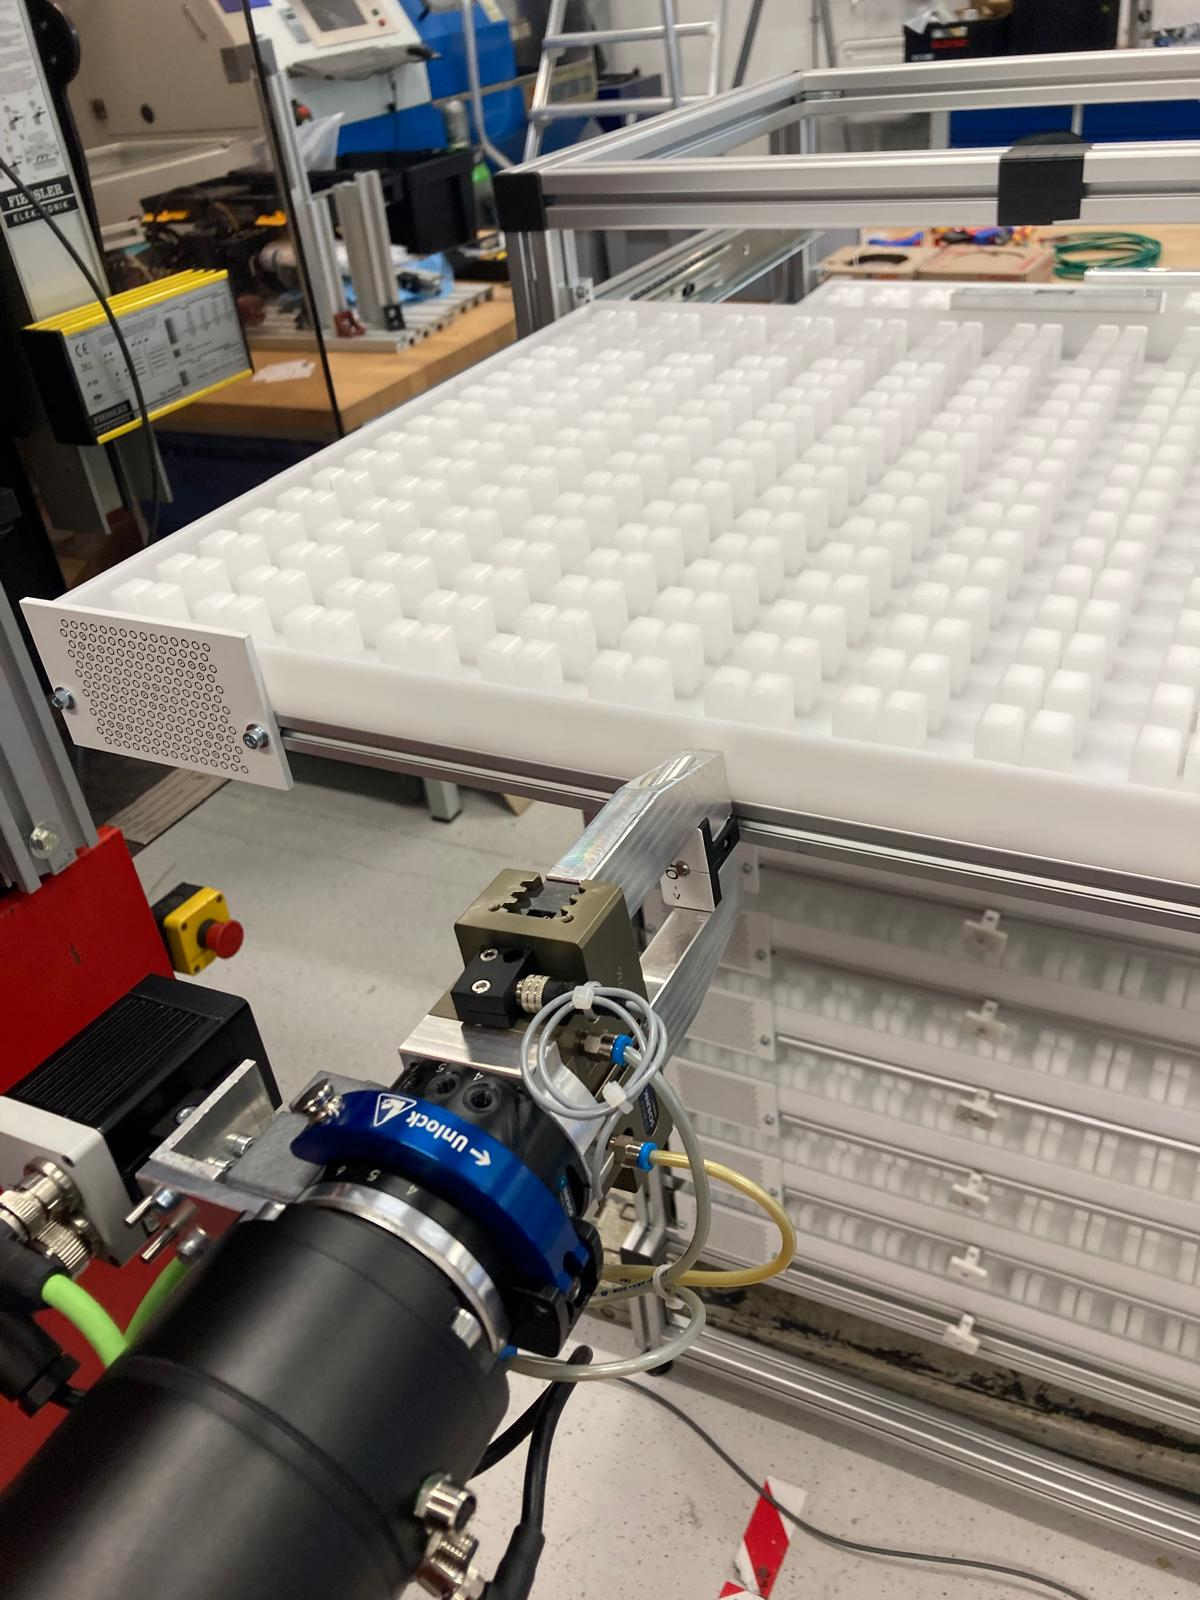
\includegraphics[width=\textwidth]{figures/shelf-control/open-drawer.jpeg}
        \caption{open drawer}
        \vspace{0.45cm}
        \label{fig:open-drawer}
    \end{subfigure}\hspace{0.1cm}
    \vspace{0.75cm}
    \begin{subfigure}[b]{0.32\textwidth}
        \centering
        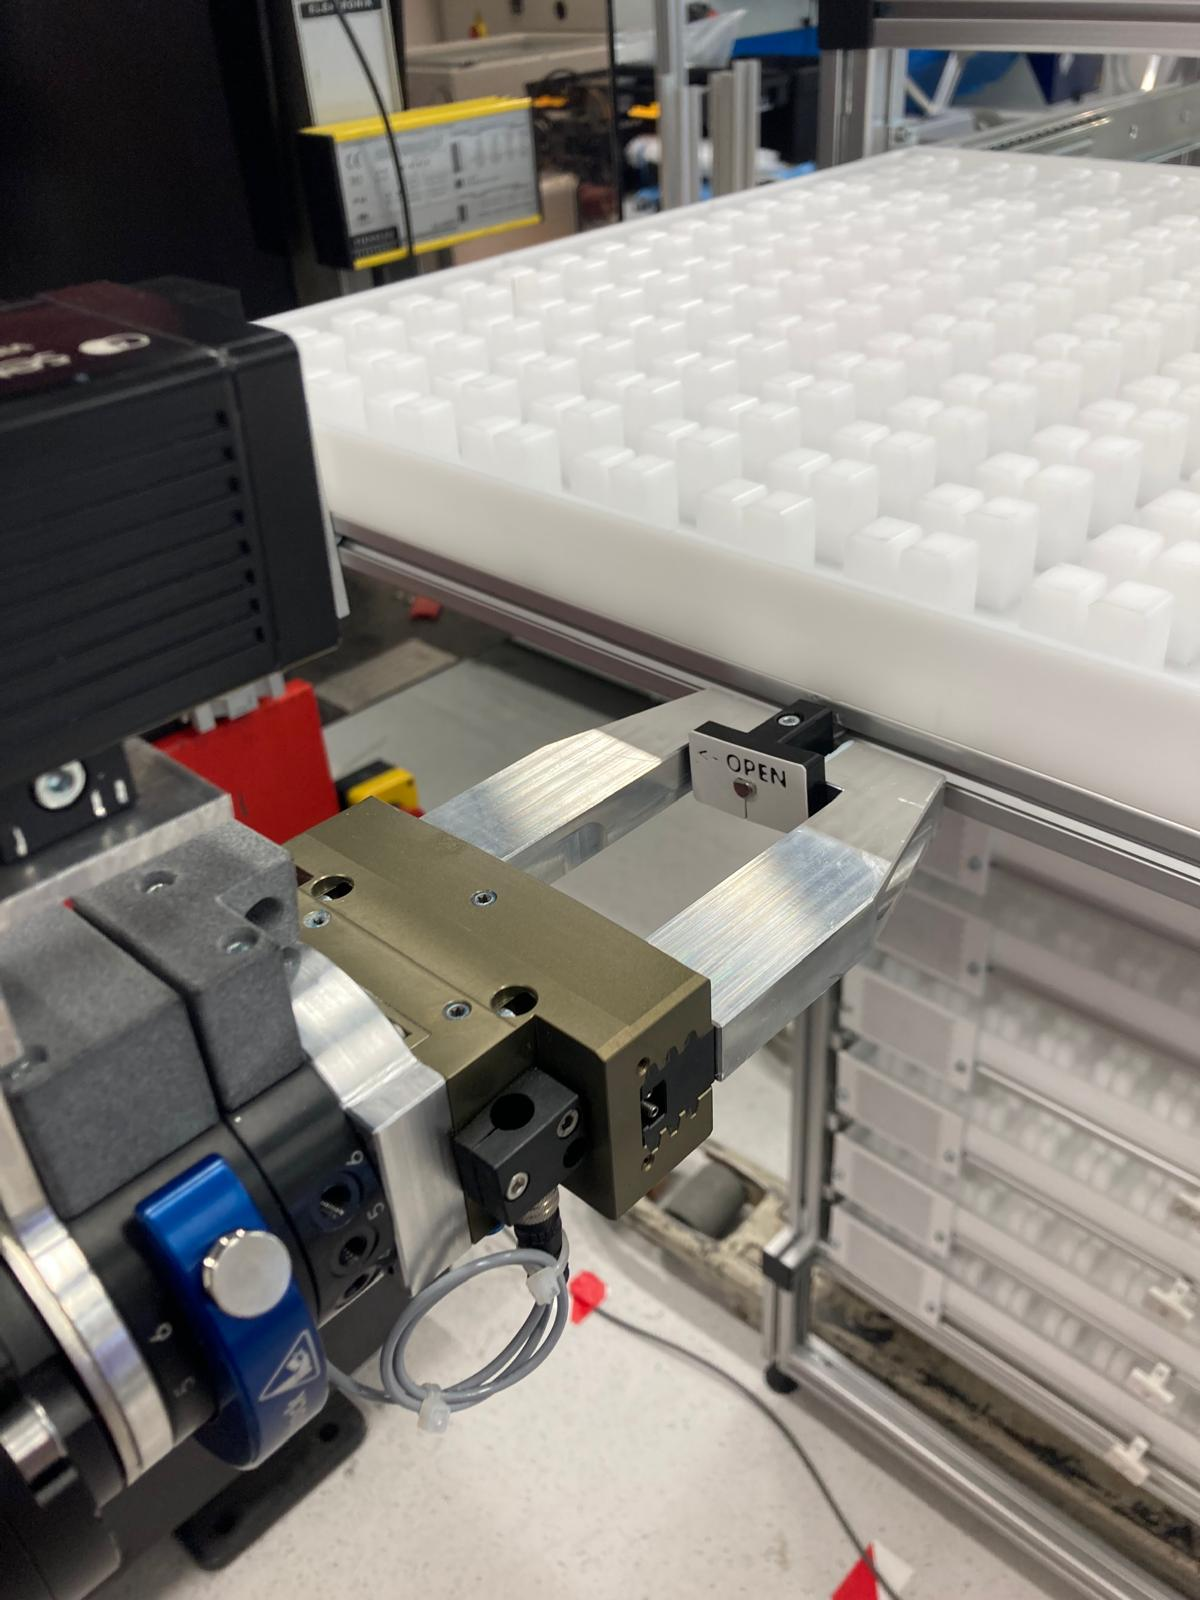
\includegraphics[width=\textwidth]{figures/shelf-control/close-handle.jpeg}
        \caption{Turn handle -100\textdegree{} to fix drawer in open position}
        \label{fig:close-handle}
    \end{subfigure}\hspace{0.1cm}
    \begin{subfigure}[b]{0.32\textwidth}
        \centering
        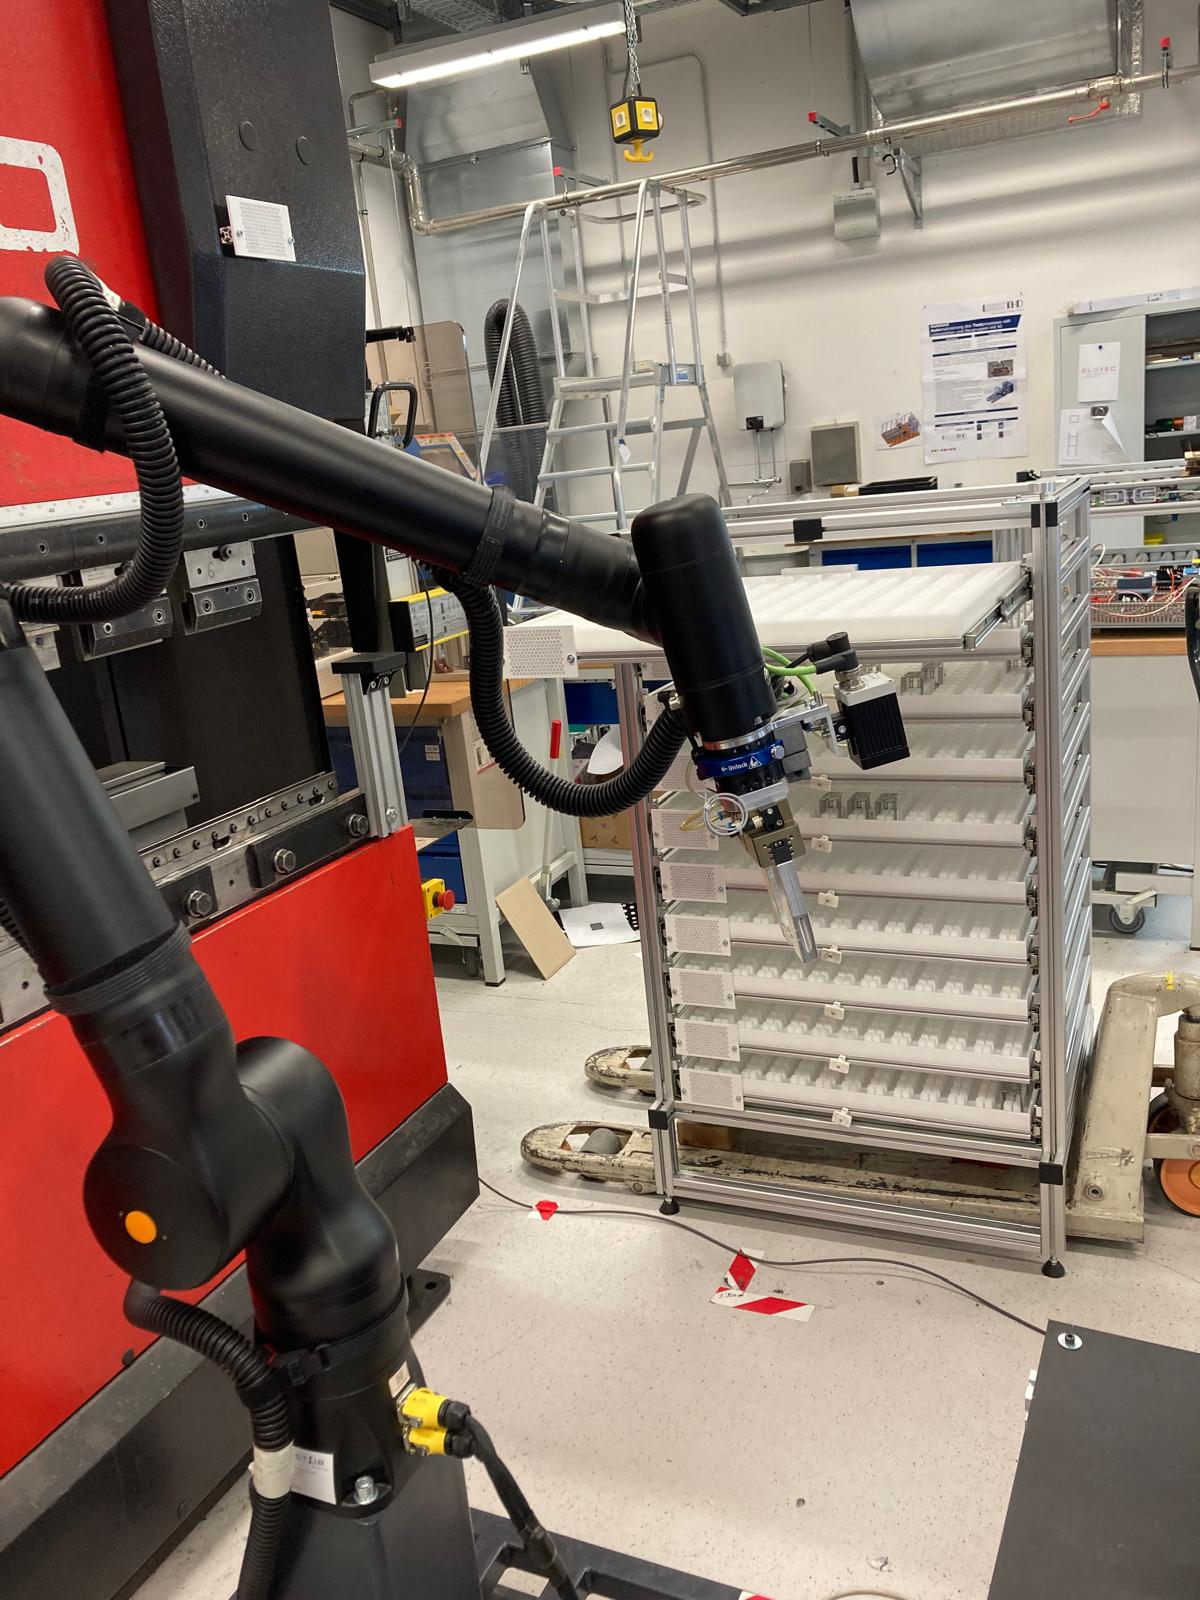
\includegraphics[width=\textwidth]{figures/shelf-control/drawer-opened.jpeg}
        \caption{Robot ready with drawer open}
        \label{subfig:drawer-opened}
    \end{subfigure}\hspace{0.1cm}
    \caption{Opening a shelf drawer for placement of bent sheet metal parts}
    \label{fig:shelf-control}
\end{figure}



\FloatBarrier  % Force all figures of the first section to be placed before the next section
